% Options for packages loaded elsewhere
\PassOptionsToPackage{unicode}{hyperref}
\PassOptionsToPackage{hyphens}{url}
\PassOptionsToPackage{dvipsnames,svgnames,x11names}{xcolor}
%
\documentclass[
  12pt,
  a4paper,
  DIV=11,
  numbers=noendperiod]{scrartcl}

\usepackage{amsmath,amssymb}
\usepackage{iftex}
\ifPDFTeX
  \usepackage[T1]{fontenc}
  \usepackage[utf8]{inputenc}
  \usepackage{textcomp} % provide euro and other symbols
\else % if luatex or xetex
  \usepackage{unicode-math}
  \defaultfontfeatures{Scale=MatchLowercase}
  \defaultfontfeatures[\rmfamily]{Ligatures=TeX,Scale=1}
\fi
\usepackage{lmodern}
\ifPDFTeX\else  
    % xetex/luatex font selection
  \setmainfont[]{Times New Roman}
\fi
% Use upquote if available, for straight quotes in verbatim environments
\IfFileExists{upquote.sty}{\usepackage{upquote}}{}
\IfFileExists{microtype.sty}{% use microtype if available
  \usepackage[]{microtype}
  \UseMicrotypeSet[protrusion]{basicmath} % disable protrusion for tt fonts
}{}
\makeatletter
\@ifundefined{KOMAClassName}{% if non-KOMA class
  \IfFileExists{parskip.sty}{%
    \usepackage{parskip}
  }{% else
    \setlength{\parindent}{0pt}
    \setlength{\parskip}{6pt plus 2pt minus 1pt}}
}{% if KOMA class
  \KOMAoptions{parskip=half}}
\makeatother
\usepackage{xcolor}
\usepackage[top=20mm,left=20mm,heightrounded]{geometry}
\setlength{\emergencystretch}{3em} % prevent overfull lines
\setcounter{secnumdepth}{5}
% Make \paragraph and \subparagraph free-standing
\ifx\paragraph\undefined\else
  \let\oldparagraph\paragraph
  \renewcommand{\paragraph}[1]{\oldparagraph{#1}\mbox{}}
\fi
\ifx\subparagraph\undefined\else
  \let\oldsubparagraph\subparagraph
  \renewcommand{\subparagraph}[1]{\oldsubparagraph{#1}\mbox{}}
\fi


\providecommand{\tightlist}{%
  \setlength{\itemsep}{0pt}\setlength{\parskip}{0pt}}\usepackage{longtable,booktabs,array}
\usepackage{calc} % for calculating minipage widths
% Correct order of tables after \paragraph or \subparagraph
\usepackage{etoolbox}
\makeatletter
\patchcmd\longtable{\par}{\if@noskipsec\mbox{}\fi\par}{}{}
\makeatother
% Allow footnotes in longtable head/foot
\IfFileExists{footnotehyper.sty}{\usepackage{footnotehyper}}{\usepackage{footnote}}
\makesavenoteenv{longtable}
\usepackage{graphicx}
\makeatletter
\def\maxwidth{\ifdim\Gin@nat@width>\linewidth\linewidth\else\Gin@nat@width\fi}
\def\maxheight{\ifdim\Gin@nat@height>\textheight\textheight\else\Gin@nat@height\fi}
\makeatother
% Scale images if necessary, so that they will not overflow the page
% margins by default, and it is still possible to overwrite the defaults
% using explicit options in \includegraphics[width, height, ...]{}
\setkeys{Gin}{width=\maxwidth,height=\maxheight,keepaspectratio}
% Set default figure placement to htbp
\makeatletter
\def\fps@figure{htbp}
\makeatother
% definitions for citeproc citations
\NewDocumentCommand\citeproctext{}{}
\NewDocumentCommand\citeproc{mm}{%
  \begingroup\def\citeproctext{#2}\cite{#1}\endgroup}
\makeatletter
 % allow citations to break across lines
 \let\@cite@ofmt\@firstofone
 % avoid brackets around text for \cite:
 \def\@biblabel#1{}
 \def\@cite#1#2{{#1\if@tempswa , #2\fi}}
\makeatother
\newlength{\cslhangindent}
\setlength{\cslhangindent}{1.5em}
\newlength{\csllabelwidth}
\setlength{\csllabelwidth}{3em}
\newenvironment{CSLReferences}[2] % #1 hanging-indent, #2 entry-spacing
 {\begin{list}{}{%
  \setlength{\itemindent}{0pt}
  \setlength{\leftmargin}{0pt}
  \setlength{\parsep}{0pt}
  % turn on hanging indent if param 1 is 1
  \ifodd #1
   \setlength{\leftmargin}{\cslhangindent}
   \setlength{\itemindent}{-1\cslhangindent}
  \fi
  % set entry spacing
  \setlength{\itemsep}{#2\baselineskip}}}
 {\end{list}}
\usepackage{calc}
\newcommand{\CSLBlock}[1]{\hfill\break\parbox[t]{\linewidth}{\strut\ignorespaces#1\strut}}
\newcommand{\CSLLeftMargin}[1]{\parbox[t]{\csllabelwidth}{\strut#1\strut}}
\newcommand{\CSLRightInline}[1]{\parbox[t]{\linewidth - \csllabelwidth}{\strut#1\strut}}
\newcommand{\CSLIndent}[1]{\hspace{\cslhangindent}#1}

\KOMAoption{captions}{tableheading}
\usepackage{wrapfig}
\usepackage{subcaption}
\usepackage{amsmath}
\usepackage{cancel}
\usepackage{hyperref}
\usepackage{tikz}
\usepackage{setspace}
\setstretch{1.5}
\usetikzlibrary{shapes.geometric, arrows, arrows.meta, positioning, calc}
\usepackage{tabularx}
\renewcommand{\maketitle}{}
\usepackage{fancyhdr}
\pagestyle{fancy}
\fancyhf{}
\fancyhead[L]{\rightmark}
\fancyhead[R]{\thepage}
\fancyfoot[C]{\thepage}
\usepackage{colortbl}
\definecolor{cornflowerblue}{RGB}{100,149,237}
\definecolor{darkblue}{RGB}{115,150,255}
\definecolor{lighterblue}{RGB}{131, 191, 212}
\definecolor{lightblue}{RGB}{178,211,220}
\makeatletter
\@ifpackageloaded{caption}{}{\usepackage{caption}}
\AtBeginDocument{%
\ifdefined\contentsname
  \renewcommand*\contentsname{Table of contents}
\else
  \newcommand\contentsname{Table of contents}
\fi
\ifdefined\listfigurename
  \renewcommand*\listfigurename{Figurliste}
\else
  \newcommand\listfigurename{Figurliste}
\fi
\ifdefined\listtablename
  \renewcommand*\listtablename{Tabelliste}
\else
  \newcommand\listtablename{Tabelliste}
\fi
\ifdefined\figurename
  \renewcommand*\figurename{Figur}
\else
  \newcommand\figurename{Figur}
\fi
\ifdefined\tablename
  \renewcommand*\tablename{Tabell}
\else
  \newcommand\tablename{Tabell}
\fi
}
\@ifpackageloaded{float}{}{\usepackage{float}}
\floatstyle{ruled}
\@ifundefined{c@chapter}{\newfloat{codelisting}{h}{lop}}{\newfloat{codelisting}{h}{lop}[chapter]}
\floatname{codelisting}{Listing}
\newcommand*\listoflistings{\listof{codelisting}{List of Listings}}
\makeatother
\makeatletter
\makeatother
\makeatletter
\@ifpackageloaded{caption}{}{\usepackage{caption}}
\@ifpackageloaded{subcaption}{}{\usepackage{subcaption}}
\makeatother
\ifLuaTeX
  \usepackage{selnolig}  % disable illegal ligatures
\fi
\usepackage{bookmark}

\IfFileExists{xurl.sty}{\usepackage{xurl}}{} % add URL line breaks if available
\urlstyle{same} % disable monospaced font for URLs
\hypersetup{
  colorlinks=true,
  linkcolor={blue},
  filecolor={Maroon},
  citecolor={Blue},
  urlcolor={Blue},
  pdfcreator={LaTeX via pandoc}}

\author{}
\date{}

\begin{document}


\newgeometry{left=0cm, right=0cm, top=0cm, bottom=0cm}
\vspace*{0.5cm} 
\hspace*{1.5cm}
\includegraphics[width=10cm]{dokumentobjekter/texstuff/UiT_Logo_Bok_Bla_RGB.png} 


\begin{flushleft}
    \vspace*{0.5cm}
    \hspace*{2.5cm}\large{\color{black}\textbf{Formuefordeling og sykefravær}}  \\[0.5em]
\hspace*{2.5cm}\color{black}\fontsize{11}{13.2}\selectfont  Daniel Nikolai Johannessen og Daniel Fabio Groth \\[0.5em]
    \hspace*{2.5cm}{\color{black}\fontsize{11}{13.2}\selectfont Handelshøgskolen ved UiT \\[0.2em]
    \hspace*{2.5cm}\color{black}\fontsize{11}{13.2}\selectfont Juni 2025 \\[0.5em]
    \hspace*{2.0cm}
    \par}
\end{flushleft} 



\begin{tikzpicture}[remember picture, overlay]
    \node[anchor=south west, inner sep=0] at (current page.south west) {
\includegraphics[width=\paperwidth]{dokumentobjekter/texstuff/forside_bilde.png}};
\end{tikzpicture}


\newgeometry{left=20mm, right=20mm, top=20mm, bottom=20mm}




\thispagestyle{plain}
\begin{center}
    \Large
    \textbf{Forord}
\end{center}

Vi vil takke vår veileder Espen Sirnes for strålende veiledning og
flotte samtaler på kontoret.

\newpage
\hypersetup{linkcolor=black}
\renewcommand{\contentsname}{Innholdsfortegnelse}
\renewcommand*{\figureautorefname}{Figur}
\renewcommand*{\tableautorefname}{Tabell}
\renewcommand*{\equationautorefname}{Ligning:}
\tableofcontents
\listoffigures
\listoftables
\hypersetup{linkcolor=blue}
\newpage
\thispagestyle{plain}
\begin{center}
    \Large
    \textbf{Sammendrag}
\end{center}

Sammendrag her

Husk å nevne at vi fjernet alle de som hadde over 14 dager
sammenhengende sykefravær

Nevne fjerning av Tilbakemelding\_sjef, Arbeidsresultater ETTER og ha
testet.

Stotte\_sjef

Stotte\_kollega

\newpage

\section{Innledning}\label{innledning}

Denne bacheloroppgaven undersøker sammenhengen mellom sosioøkonomiske
forhold og sykefravær, med et spesielt fokus på hvordan endringer i
formuefordeling kan påvirke arbeidstakeres helse og fravær fra jobben.
Vi benytter en Job Demands-Resources (JD-R)-modell som teoretisk
rammeverk, og analyserer data fra Levekårsundersøkelsen om arbeidsmiljø.

\subsubsection{Bakgrunn}\label{bakgrunn}

I årene etter finanskrisen har vi observert en økende formueulikhet i
mange vestlige land, inkludert Norge. (Zucman, 2019) Denne trenden kan
være forsterkende av Gatsby-kurven\footnote{Gatsby-kurven viser en
  sammenheng mellom økonomisk ulikhet og redusert sosial mobilitet.
  Durlauf et al. (2022)} og har blitt enda sterkere etter pandemien.
Spesielt i boligmarkedet, hvor vi ser at lønnsveksten ikke har holdt
tritt med prisøkningen på eiendeler. Dette har gjort det relativt
vanskeligere for unge og de med lavere inntekter å opparbeide seg
formue, for eksempel gjennom boligkjøp.

Formue fungerer som en buffer mot levekårsproblemer og det å ta hensyn
til formue gir et bedre syn på hvor økonomisk utsatt personer er enn kun
inntektsmål. Hattrem (n.d.)

Vi forventer dermed at formuenivået til arbeidstakere har en effekt på
spesielt motivasjon og helse, og dermed påvirker sykefraværet. Når det
blir stadig vanskeligere å oppnå økonomisk trygghet og en akseptabel
levestandard, kan det føre til økt stress, redusert jobbmotivasjon, og i
verste fall dårligere helse og økt fravær. Hypotesene våre er basert på
Job Demands-Resources (JD-R-modellen), som antyder at jobbkrav og
jobbressurser påvirker sykefravær, og at formue kan moderere disse
effektene. Hovedsakelig vil vi se på hvordan formue påvirker sykefravær,
og der forventer vi at høyere formue gir lavere sykefravær og at høyere
formue demper de negative effektene av jobbkrav og forsterker de
positive effektene av jobbressurser.

Å forstå hvordan disse endringene påvirker arbeidstakeres helse og
fravær er viktig for å kunne iverksette tiltak som kan motvirke negative
konsekvenser av økende formueulikhet. Dette kan være spesielt viktig i
en tid hvor vi ser en økende polarisering i samfunnet, og hvor det er
viktig å sikre at alle har like muligheter til å oppnå økonomisk
trygghet og god helse, uavhengig av formue og inntekt. Problemstillingen
for oppgaven er dermed: \emph{Forklarer nivået på formue sykefraværet i
Norge?}. Vi vil undersøke om forskjellige formuegrupper har ulikt
sykefravær, og om det er en sammenheng mellom formue og sykefravær. Vi
vil også se på om det er andre faktorer som påvirker sykefraværet, og om
disse faktorene kan forklare eventuelle sammenhenger mellom formue og
sykefravær. Vi vil danne oss flere hypoteser basert på teori og
tidligere forskning, og teste disse ved hjelp av en Structural Equation
Model (SEM), hvor vi kontrollerer for andre relevante faktorer, som for
eksempel alder, kjønn, utdanning og yrke.

Tidligere forskning har funnet at sosioøkonomiske forhold, som inntekt
og utdanning, har en effekt på helse og sykefravær. Jaeggi et al. (2021)
testet dette på et lite samfunn av innfødte i Tsimane i Bolivia, hvor de
fant at økt formue hadde en positiv effekt på helse, mens større ulikhet
ledet til respirasjonssykdom som førte til økt dødlighet.

I teorien starter vi med å gå gjennom begrepsavklaringer, hvor vi vil
definere formue, sykefravær og andre relevante begreper. Deretter vil vi
gå dypere inn i tidligere forskning på temaet, og se på tidligere funn,
og hvilke mekanismer som kan forklare sammenhengen mellom formue og
sykefravær.

\subsubsection{Oppsett}\label{oppsett}

Oppgaven er delt inn i følgende kapitler: I kapittel 2 vil vi gi en
teoretisk bakgrunn for oppgaven, og gjøre rede for tidligere forskning
på temaet. I kapittel 3 vil vi forklare metode og datagrunnlag, i
kapittel 4 gjennomføres analysen og i kapittel 5 vil vi presentere
resultatene fra analysen. Avslutningsvis i kapittel 6 vil vi diskutere
resultatene, konkludere og gi anbefalinger for videre forskning.

\section{Teori \{sec:teori\}}\label{teori-secteori}

I dette kapittelet vil vi gi en teoretisk bakgrunn for oppgaven, og
gjøre rede for tidligere forskning på temaet. Vi vil først definere
begrepene kortfattet, og deretter presentere teori og empiri som er
relevant for oppgaven. Vi vil spesielt fokusere på JD-R-modellen, som er
et mye brukt rammeverk for å forstå sammenhengen mellom arbeidsmiljø og
helse.

\subsection{Begrepsdefinisjoner}\label{begrepsdefinisjoner}

\subsubsection{Formue
(bruttofinanskapital)}\label{formue-bruttofinanskapital}

Formue er et begrep som refererer til den totale verdien av eiendeler og
investeringer som en person eller husholdning eier. Dette inkluderer
kontanter, eiendom, aksjer, obligasjoner og andre finansielle eiendeler.
Formue kan også referere til nettoformue, som er forskjellen mellom
eiendeler og gjeld.

I studien vår vil vi bruke variabelen bruttofinanskapital\footnote{Definisjon
  for bruttofinanskapital fra
  \href{https://www.ssb.no/a/metadata/conceptvariable/vardok/3449/nb}{SSB}}
som en proxy for formue. Bruttofinanskapital omfatter bankinnskudd,
andeler i aksje-,obligasjons- og pengefond, aksjer og obligasjons- og
pengemarkedsfond, formue i aksjesparekonto, obligasjoner, aksjer og
andre verdipapirer. (SSB, 2017) Som beskrevet i Normann (2009) fungerer
formue som en buffer mot levekårsproblemer, og det er denne bufferen vi
antar er sentral for hvordan arbeidstakere håndterer jobbrelaterte
utfordringer. Vi blir å bruke formue som en forventet moderator i vår
analyse, og vil da se hvordan formue påvirker sykefraværet.

\subsubsection{Sykefravær}\label{sykefravuxe6r}

Sykefravær\footnote{Definisjon for sykefravær fra
  \href{https://www.ssb.no/arbeid-og-lonn/arbeidsmiljo-sykefravaer-og-arbeidskonflikter/statistikk/sykefravaer}{SSB}.}
refererer til perioden en ansatt er borte fra jobb på grunn av sykdom
eller skade dokumentert med egenmelding eller legemelding, i henhold til
norske lover og avtaler. (SSB,2025)

I vår analyse vil vi bruke en selvberegnet sykefraværsprosent som
avhengig variabel for 2022. Levekårsundersøkelsen inneholder ferdig
aggregerte variabler for fravær, men for å ta sikre at målingen vår
reflekterer fravær i forhold til den enkeltes avtalte arbeidsmengde så
velger vi å lage dette målet selv. Vi benytter sykefraværsdagsverk i
2022 og avtalte dageverk, uten feriekorrigering fra datasettet.
Sykefraværsprosenten (\(SF_i\)) for individ i defineres dermed som:

\[
SF_i = \frac{ \text{Antall sykefraværsdager}}{\text{Antall avtalte dagsverk}} 
\] Dette gir oss et persontilpasset mål på sykefravær som tar høyde for
individuelle arbeidsavtaler.

\subsubsection{Jobbkrav}\label{jobbkrav}

Jobbkrav refererer til de kravene og utfordringene som ansatte må gjøre
i jobben. Mer spesifikt, så refereres det til de fysiske, psykologiske,
sosiale og organisatoriske kravene som stilles til ansatte i løpet av
arbeidsdagen, og som derfor assosieres med fysiologiske eller
psykologiske kostnader.(Schaufeli \& Bakker, 2004)

Jobbkrav kan være både fysiske og psykiske, og kan inkludere krav som
arbeidsmengde, tidsfrister, ansvar, og emosjonelle krav. Jobbkrav kan
føre til stress og utbrenthet, og kan påvirke jobbengasjement og trivsel
negativt.

I vår analyse vil vi gjøre jobbkrav om til en latent\footnote{En latent
  variabel er et underliggende, uobserverbart konstrukt som ikke kan
  måles direkte, men som modelleres gjennom flere målbare indikatorer. I
  SEM tolkes for eksempel «motivasjon», «jobbkrav» og «jobbressurser»
  som latente variabler: Vi antar at variasjonen i et sett av
  attestspørsmål (indikatorer) reflekterer den samme underliggende
  faktoren.} variabel som består av flere observerbare variabler. I
denne variabelen vil vi inkludere variabler som måler arbeidsmengde,
arbeidstempo og hvor mye ekstra arbeid som kreves i jobb.

\subsubsection{Jobbressurser}\label{jobbressurser}

Jobbressurser refererer til de fysiske og psykologiske, sosiale eller
organisatoriske aspektene ved jobben som bidrar til å redusere jobbkrav
og de assosierte psykologiske og fysiologiske kostnadene. Jobbressurser
kan også bidra til å oppnå arbeidsmål, fremme personlig vekst og
utvikling, og øke jobbengasjement og trivsel. Jobbressurser kan være
både interne og eksterne, og kan inkludere faktorer som støtte fra
kolleger og ledelse, muligheter for utvikling og læring, autonomi i
arbeidet, og fleksibilitet i arbeidsoppgaver. (Schaufeli \& Bakker,
2004)

Vi blir å bruke jobbressurser som en latent variabel som består av
følgende observerbare variabler: støtte fra sjef, støtte fra kolleger,
grad av selvbestemmelse i oppgaver og arbeid som skal gjøres, grad av
arbeidstempo og grad av påvirkning på beslutninger i arbeidet.

\subsubsection{Motivasjon}\label{motivasjon}

Motivasjon\footnote{Per definisjon av
  \href{https://snl.no/motivasjon\#:~:text=Motivasjon\%20er\%20en\%20samlebetegnelse\%20for,motiveres\%20til\%20\%C3\%A5\%20oppn\%C3\%A5\%20dette}{SNL}.}
refererer til de indre og ytre faktorene som igangsetter og styrer
atferd og mennesker og dyr. Motivasjon kan være både indre (for eksempel
personlig interesse eller glede ved å utføre oppgaven) og ytre (for
eksempel belønninger eller anerkjennelse fra andre). Motivasjon kan
derfor påvirke jobbengasjement, trivsel og sykefravær.

\subsection{Job Demands-Resources (JD-R
modellen)}\label{job-demands-resources-jd-r-modellen}

Job Demands-Resources-modellen ble først beskrevet av Demerouti et al.
(2001) som et rammeverk for å forstå hvordan arbeidsmiljøet påvirker
helse og trivsel. Modellen skiller mellom to typer faktorer: jobbkrav
(job demands) og jobbressurser (job resources). Jobbkrav refererer til
kravene og utfordringene som ansatte møter i jobben, mens jobbressurser
refererer til de ressursene og støtten som ansatte har tilgjengelig for
å håndtere disse kravene. Modellen antyder at en balanse mellom jobbkrav
og jobbressurser er viktig for å opprettholde helse og trivsel på
arbeidsplassen. Høyere jobbkrav kan føre til stress og utbrenthet, mens
høyere jobbressurser kan føre til økt motivasjon og trivsel.

Grunnen til at vi velger JD-R modellen er fordi vi forventer at
formuenivå kan forandre jobbkrav og jobbressurser. Vi tenker også at
formuenivået har mye å si til hvordan jobbkrav og jobbressurser påvirker
personer.

I \autoref{fig:jdr_tikzz} ser vi en presentasjon av JD-R-modellen.
Jobbkravene og jobbressursene påvirker sykefraværet gjennom motivasjon.
Vi antyder at jobbkravene har en negativ effekt på motivasjon, mens
jobbressursene blir å ha en positiv effekt på motivasjon. Og dermed
antar vi at sykefraværet også påvirkes av motivasjonen, hvor høyere
motivasjon vil føre til lavere sykefravær.

\begin{figure}
  \centering
  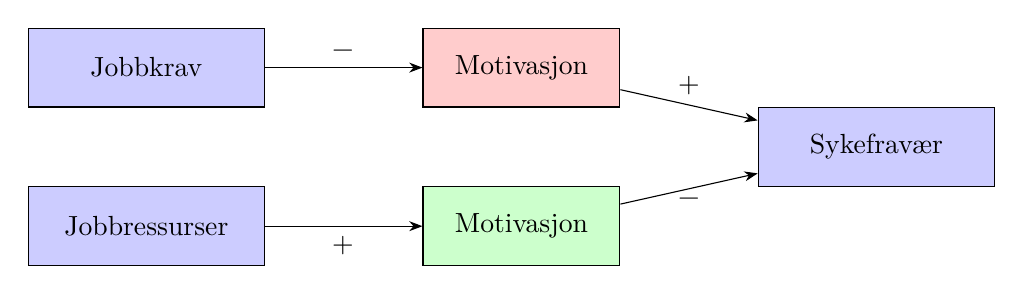
\begin{tikzpicture}[
      latent/.style={rectangle, draw, fill=blue!20, minimum width=3cm, minimum height=1cm},
      item/.style  ={rectangle, draw, fill=blue!10, font=\small},
      medi/.style  ={rectangle, draw, fill=green!20, minimum width=2.5cm, minimum height=1cm},
      medi2/.style ={rectangle, draw, fill=red!20,   minimum width=2.5cm, minimum height=1cm},
      moder/.style ={diamond,   draw, fill=yellow!20,aspect=2, minimum width=2.5cm, minimum height=1cm},
      >=Stealth,
      node distance=1cm and 2cm
    ]

    % Latente noder
    \node[latent]              (JK)  {Jobbkrav};
    \node[latent, below=of JK] (JR)  {Jobbressurser};

    % To separate motivasjons-noder
    \node[medi2, right=of JK] (M1) {Motivasjon};
    \node[medi,  right=of JR] (M2) {Motivasjon};

    % Piler fra latente til motivasjon med tegn
    \draw[->] (JK) -- node[midway, above] {$-$} (M1);
    \draw[->] (JR) -- node[midway, below] {$+$} (M2);

    % Sykefravær
    \node[latent, right=3cm of $(M1)!0.5!(M2)$] (SF) {Sykefravær};

    % Piler fra motivasjon til sykefravær med tegn
    \draw[->] (M1) -- node[midway, above] {$+$} (SF);
    \draw[->] (M2) -- node[midway, below] {$-$} (SF);

  \end{tikzpicture}
  \caption{JD–R-modellen}
  \label{fig:jdr_tikzz}
\end{figure}

Schaufeli \& Bakker (2004) testet i en SEM-analyse hvordan jobbkrav og
jobbressurser forklarer utbrenthet og jobbengasjement. Studien viste at
utbrenthet og jobbengasjement var negativt korrelert, og at jobbkravene
hadde en positiv effekt på utbrenthet, mens jobbressursene hadde en
signifikant \textbf{positiv} effekt på jobbengasjement. Dette kan
understøtte at høye krav skaper stress og fravær, mens ressurser fremmer
engasjement og opplevelse av mestring. Denne studien fokuserer på
hvordan utbrenthet har en medierende effekt på forholdet mellom jobbkrav
og helseproblemer, og engasjement medierer forholdet til jobbressurser
og intensjon om å slutte i arbeid. Studien deres inkluderte kun
respondenter fordelt på fire forskjellige arbeidsplasser og yrker, og vi
vil da videre fokusere på hvordan jobbkrav og jobbressurser påvirker
sykefravær gjennom motivasjon, og hvordan formue kan moderere disse
effektene for arbeidstakere i hele Norge.

\subsubsection{Formue i JD-R}\label{sec-formue-jdr}

Vi mener at økonomiske ressurser som formue, kan hjelpe med å forklare
sykefraværet enda mer og vil bruke den som en ekstern modererende
faktor.

Hobfoll (1989) definerer jobbressurser som ressurser som kan hjelpe
individer med å håndtere jobbkrav og da kan fungere som en buffer for
stress i hans Conversation of Resources (COR)-teori. Formue gir da en
økonomisk buffer som kan redusere sårbarheten for jobbrelatert stress.
Personer med høy formue kan ha større valgfrihet i arbeidslivet, og
tåler lettere perioder med høy belastning uten at det går like hardt
utover helse eller jobbmotivasjon. Dermed antyder vi at personer med lav
eller negativ formue vil ofte være mer økonomisk avhengige av inntekten
fra arbeid, og kan derfor være mer sårbare for jobbrelatert stress.

Formue kan også ha betydning for fremtidsperspektiv og indre motivasjon.
Personer med lav formue kan oppleve mindre kontroll over egen
livssituasjon og lavere forventninger til fremtidig økonomisk trygghet,
noe som potensielt svekker arbeidsglede og motivasjon.

Vi antar da at formue påvirker hvordan individet opplever og håndterer
jobbkrav og jobbressurser. Vi postulerer at formue fungerer som en
moderator for sensitiviteten til endringer i arbeidsforhold og inntekt.
En person med lav formue kan være mer sensitiv for både negative og
positive endringer i jobbkrav og jobbressurser siden den økonomiske
marginen er mindre. Motsatt kan en person med høy formue være mindre
sensitiv for endringer i jobbkrav og jobbressurser, og dermed oppleve
mindre stress og utbrenthet. Dette kan føre til at personer med høy
formue er mer motstandsdyktige mot negative effekter av jobbkrav og mer
mottakelige for positive effekter av jobbressurser. Dette kan bety at
effekten er ikke-lineær eller bue formet, hvor effekten er sterkest i de
med lavest formue og avtar med økende formue. Hvis det er
motivasjonsmessige effekter av formuenivå så kan det være at et lavt
formuenivå vil gjøre en mindre motivert og indirekte påvirke sykefravær,
men også fungere motsatt ved høy formue.

Denne antagelsen støttes av Üngüren et al. (2021) hvor de fant at
økonomisk velvære\footnote{Økonomisk velvære kan defineres som en
  tilstand der en person fullt ut kan møte nåværende og løpende
  økonomiske forpliktelser, kan føle seg trygg på sin økonomiske
  fremtid, og er i stand til å ta valg som gjør det mulig å nyte livet.
  Financial Protection Bureau) (2015)} fungerte som en moderator som
reduserte den negative effekten av jobbusikkerhet på utbrenthet blant
hotellansatte.

Ved å inkludere formue som en ekstern faktor i JD-R-modellen, forsøker
vi å fange både den direkte effekten av økonomisk trygghet og hvordan
denne tryggheten forsterker eller demper effektene av jobbrelaterte
faktorer. I et samfunn med økende økonomisk ulikheter hvor forskjellen
mellom dem som har og dem som ikke har, blir større og større, er det
viktig å forstå hvordan dette påvirker arbeidstakere og deres helse. Så
derfor antar vi at formue vil kunne forsterke effektene av jobbressurser
og fungere som en buffer mot jobbkrav, og dermed påvirke sykefraværet i
Norge.

\subsection{Tidligere forskning}\label{tidligere-forskning}

Tidligere empirisk forskning har over tid vist positive forhold mellom
forskjellige Job Demands-Resources-faktorer og årsaker som kan føre til
sykefravær.

\subsubsection{Mikronivå: JD-R-studier i helse- og
omsorgssektoren}\label{mikronivuxe5-jd-r-studier-i-helse--og-omsorgssektoren}

Vander Elst et al. (2016) brukte en JD-R-modell hvor de utførte en
SEM-analyse på Belgisk hjemme-pleiepersonell. Jobbkrav og jobbressurser
ble modellert som prediktorer. Studien viste at jobbkravene var positivt
assosiert med utbrenthet, mens jobbressursene var positivt assosiert med
jobbengasjement. Denne studien viser også at JDR-mekanismer holder i
andre sammenhenger hvor arbeidstakere er under emosjonelt press og
skiftarbeid, noe som impliserer at JDR-modellen er robust på tvers av
sektorer og bransjer.

\subsubsection{Mikronivå:
formue-helse-koblinger}\label{mikronivuxe5-formue-helse-koblinger}

Jaeggi et al. (2021) undersøkte effekten av ulikhet i formue i et
småskala samfunn av innfødte i Tsimane i Bolivia med 871 observasjoner,
\(n = 871\). I studien testet de relativ husholdningrikdom og ulikhet i
formue mot forskjellige psykologiske variabler og helseutfall som
depresjon, BMI, blodtrykk og sykelighet.

Studien viste til en kobling mellom formueulikhet hvor de med lavere
formue hadde større sannsynlighet for å få høyere blodtrykk og
luftveissykdommer som kunne lede til dødsfall. De fant også at de med
høyere formue hadde lavere sannsynlighet for å få depresjon og høyere
BMI. Dette indikterer at ulikhet i formue kan moderere stress og
helserisiko på individnivå og vi antar da at dette kan være overførbart
til Norge, og at formue kan moderere effekten av jobbkrav og
jobbressurser på sykefravær.

\subsubsection{Mikronivå: JD-R-studier i
Norge}\label{mikronivuxe5-jd-r-studier-i-norge}

Langseth-Eide \& Vittersø (2021) bygger videre på tidligere forskning
ved JD-R-modellen. De argumenterer for at JD-R-modellen ved tidligere
forskning har hatt fokus på organisasjonsnivået, og at det er viktig å
se på hvordan JD-R-modellen kan brukes bedre på jobbressurser,
jobbengasjement og helserelaterte utfall. De gjorde en paneldata studie
på fast ansatte i Norge med to års tidsforsinkelse med 1533 ansatte
første tidsperiode, \(n =1533\) og 1503 ansatte, \(n = 1503\) neste
tidsperiode.

Over lengre tid fant de at jobbressurser hadde en positiv effekt på
jobbengasjement, og at jobbengasjement var negativt assosiert med
sykefravær. Dette impliserer at høyere jobbressurser kan føre til høyere
jobbengasjement, som igjen kan føre til lavere sykefravær i Norge, og
derfor vil vi bygge videre på denne studien ved å inkludere formue som
en moderator i JD-R-modellen.

\subsubsection{Makronivå: Ulikhet i
samfunnet}\label{makronivuxe5-ulikhet-i-samfunnet}

JD-R-modellen operer primært på individnivå, men en makroøkonomisk
studie om inntektsulikhet har vist at økonomisk ulikhet i en befolkning
korrelerer med høyere sykefravær og dårligere helse. Pickett \&
Wilkinson (2015) undersøkte sammenhengen mellom inntektsulikhet og helse
i 34 OECD-land, og fant at høyere inntektsulikhet var assosiert med
høyere sykefravær og dårligere helseutfall. Studien viste også at
inntektsulikhet hadde en negativ effekt på livskvalitet og trivsel, og
at dette kunne føre til økt sykefravær. Dette kan antas at
inntektsulikhet forsterker psykososialt stress ved lav formue, derfor
vil vi undersøke hvordan formue påvirker sykefravær i Norge, og hvordan
formue kan moderere effekten av jobbkrav og jobbressurser på sykefravær.

Mekanismene som følger på mikronivå er da:

\[
\text{Høyere jobbkrav} \rightarrow \text{Økt utbrenthet} \rightarrow \text{Høyere sykefravær} \rightarrow \text{Økt jobbengasjement} \rightarrow \text{Lavere sykefravær}
\]

Hvor formue fungerer som en moderator ved å påvirke stress til individer
før jobbkravene utløser negative effekter på helse.

På makronivå vil samfunnsmessig ulikhet forme de jobbkrav og ressurser
som virksomheter og arbeidstakere får, og dermed styrke JDR-mekanismer,
også på tvers av sektorer og bransjer. Dermed får vi et teoretisk og
empirisk grunnlag for vår undersøkelse av at:

\[
\text{Formue} \rightarrow \text{Jobbkrav og jobbressurser} \rightarrow \text{Sykefravær i Norge}
\]

\subsection{Modelloppsett}\label{modelloppsett}

Modellen vi blir å bruke blir da som følger:

\begin{figure}
  \centering
  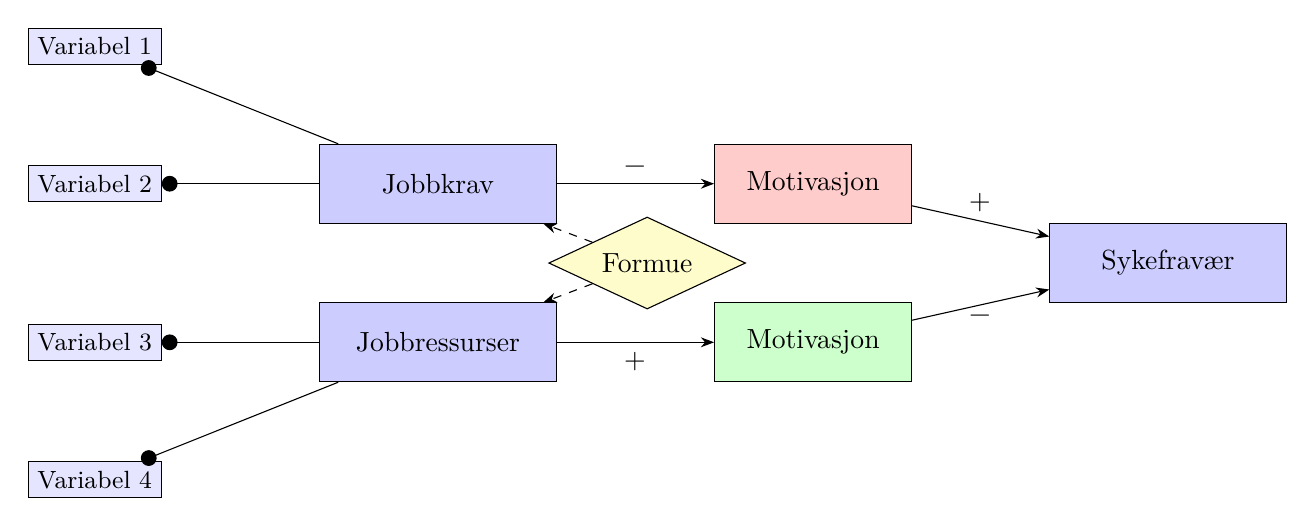
\begin{tikzpicture}[
      latent/.style={rectangle, draw, fill=blue!20, minimum width=3cm, minimum height=1cm},
      item/.style  ={rectangle, draw, fill=blue!10, font=\small},
      medi/.style  ={rectangle, draw, fill=green!20, minimum width=2.5cm, minimum height=1cm},
      medi2/.style ={rectangle, draw, fill=red!20,   minimum width=2.5cm, minimum height=1cm},
      moder/.style ={diamond,   draw, fill=yellow!20,aspect=2, minimum width=2.5cm, minimum height=1cm},
      >=Stealth,
      node distance=1cm and 2cm
    ]

    % Latente noder
    \node[latent]              (JK)  {Jobbkrav};
    \node[latent, below=of JK] (JR)  {Jobbressurser};

    % Indikator-noder for Jobbkrav
    \node[item, above left=of JK] (v1) {Variabel 1};
    \node[item, left=of JK]       (v2) {Variabel 2};
    \draw[-{Circle[length=2mm]}] (JK) -- (v1);
    \draw[-{Circle[length=2mm]}] (JK) -- (v2);

    % Indikator-noder for Jobbressurser
    \node[item, left=of JR]        (v3) {Variabel 3};
    \node[item, below left=of JR]  (v4) {Variabel 4};
    \draw[-{Circle[length=2mm]}] (JR) -- (v3);
    \draw[-{Circle[length=2mm]}] (JR) -- (v4);

    % Moderator-node plassert midt over
    \node[moder, right=1.4cm of $(JK)!0.5!(JR)$] (FN) {Formue};
    \draw[->, dashed] (FN) -- (JK);
    \draw[->, dashed] (FN) -- (JR);

    % To separate motivasjons-noder
    \node[medi2, right=of JK] (M1) {Motivasjon};
    \node[medi,  right=of JR] (M2) {Motivasjon};

    % Piler fra latente til motivasjon med tegn
    \draw[->] (JK) -- node[midway, above] {$-$} (M1);
    \draw[->] (JR) -- node[midway, below] {$+$} (M2);

    % Sykefravær
    \node[latent, right=3cm of $(M1)!0.5!(M2)$] (SF) {Sykefravær};

    % Piler fra motivasjon til sykefravær med tegn
    \draw[->] (M1) -- node[midway, above] {$+$} (SF);
    \draw[->] (M2) -- node[midway, below] {$-$} (SF);

  \end{tikzpicture}
  \caption{Utvidet JD–R-modell med formue som moderator og separate motivasjonsløp.}
  \label{fig:jdr_tikz}
\end{figure}

I modellen vår (\autoref{fig:jdr_tikz}) har vi inkludert formue som en
moderator som påvirker både jobbkrav og jobbressurser. Dette betyr at
formue kan endre hvordan jobbkrav og jobbressurser påvirker
sykefraværet. Vi har også separate motivasjonsløp for jobbkrav og
jobbressurser, som gjør at vi kan se hvordan motivasjon påvirkes av
begge disse faktorene. Vi antar at formuen blir å fungere som en
stress-avlastning eller buffer mot jobbkravene og forsterke effekten av
jobbressurser, og fungere som en psykologisk trygghet. Dette kan føre
til at personer med høyere formue opplever lavere sykefravær, mens de
med lavere formue kan oppleve høyere sykefravær på grunn av økt stress
og lavere tilgang til ressurser.

\subsubsection{Hypoteseliste}\label{hypoteseliste}

Med dette rammeverket formulerer vi følgende hypoteser:

\textbf{H1:} Høyere jobbkrav gir høyere sykefravær

\textbf{H2:} Høyere jobbressurser gir lavere sykefravær

\textbf{H3:} Høyere formuenivå gir lavere sykefravær

For en grundig gjennomgang av hypotesene og hvordan de er relatert til
JD-R-modellen, se kapittel \ref{sec-hypot}.

\section{Metode og data}\label{metode-og-data}

I dette kapitlet går vi gjennom datagrunnlag og metode for oppgaven. Vi
vil først forklare hvordan dataene er fremskaffet, så forklare
variablene, og til slutt forklare metoden. Vi vil også gi en innledende
oversikt over dataene, inkludert deskriptiv statistikk for alle
variablene i analysen.

I problemstillingen \emph{forklarer nivået på formue sykefraværet i
Norge?} så velger vi å bruke en Structural Equation Model fordi denne
kan bedre vise oss på hvilken måte formue påvirker sykefraværet og om
det finnes noen indirekte sammenhenger mellom variablene vi velger å
bruke, dette gjør analysen mer kompleks, men vi kan bedre peke direkte
på hvilke effekter som er positive eller negative på selve sykefraværet.

\subsection{Data}\label{data}

Dataen vi bruker er hentet fra Statistisk sentralbyrå (SSB) sin
\href{https://www.ssb.no/arbeid-og-lonn/arbeidsmiljo-sykefravaer-og-arbeidskonflikter/artikler/levekarsundersokelsen-om-arbeidsmiljo-2022}{levekårsundersøkelse
om arbeidsmiljø}, som ble gjennomført i 2022. Vedlagt følger et bilde av
kodeboken:

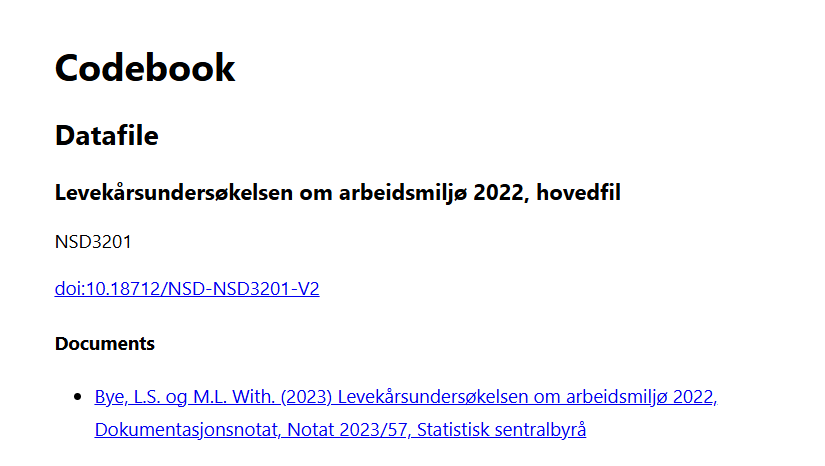
\includegraphics{dokumentobjekter/bilder/codebook.png}

Statistisk sentralbyrå har gjennomført levekårsundersøkelser siden 1973.
Levekårsundersøkelsen kartlegger arbeidsmiljøforhold blant sysselsatte i
Norge, og tar opp temaer som forhold på arbeidsplassen, fysisk,
ergonomisk og psykososialt arbeidsmiljø, yrkesrelaterte helseplager og
sykefravær og krav og muligheter for selvbestemmelse på jobb.

\subsection{Datakilde og utvalg}\label{datakilde-og-utvalg}

Undersøkelsen er basert på et landsrepresentativt utvalg på 35 345
sysselsatte personer i alderen 18-66 til undersøkelsen i 2022. Utvalget
er tilfeldig trukket fra folkeregisteret, og dataene er samlet inn
gjennom telefonintervjuer og selvadministrert webskjema fra august 2022
til april 2023.

Den totale svarprosenten for undersøkelsen var på 51 prosent, og dataene
er vektet for å være representativt for den norske befolkningen i
alderen 18-66 for å korrigere for noen av skjevhetene i forbindelse med
frafall.

\subsection{Variabler}\label{variabler}

Vi kommer til å bruke flere variabler fra levekårsundersøkelsen for å
analysere sammenhengen mellom formue og sykefravær. Vi vil bruke både
avhengige og uavhengige variabler, latente variabler, samt
kontrollvariabler for å kontrollere for andre faktorer som kan påvirke
sykefraværet.

\subsubsection{Avhengig og uavhengig
hovedvariabel}\label{avhengig-og-uavhengig-hovedvariabel}

Sykefravær:

Datasettet inneholder en ferdig variabel for sykefraværsprosent
(sfpros\_uten\_feriekorr\_2022, sfpros\_uten\_feriekorr\_2023), men vi
velger å beregne denne selv siden de med 0 fravær står som NA, også for
å kunne ta høyde for avtalt arbeidstid.

Vi benytter variablene sfdagsvj\_2022 (sykefraværsdagsverk) og
mdagsv\_2022 (avtalte dagsverk) fra Levekårsundersøkelsen.
Sykefraværsprosenten (\(SF_i\)) for individ \(i\) beregnes som:

\[
SF_i = 
\begin{cases}
0, & \text{hvis } \mathrm{mdagsv\_2022}_i > 0 \text{ og } \mathrm{sfdagsvj\_2022}_i = 0 \\
\frac{ \mathrm{sfdagsvj\_2022}_i }{ \mathrm{mdagsv\_2022}_i }, & \text{ellers}
\end{cases}
\]

Dette gjør at individer med avtalte dagsverk, men uten legemeldt
sykefraværsdager, får verdien 0 i stedet for NA slik det gjøres i den
ferdigberegnede variabelen sfpros\_uten\_feriekorr\_2022.

Formue:

Bruttofinanskapital i alt (BF) vil være vår hoveduavhengige variabel, og
vi vil bruke bruttofinanskapital i alt som mål på formue. Denne
variabelen inneholder verdien av alle finansielle eiendeler som
respondenten eier, inkludert kontanter, aksjer, obligasjoner og andre
investeringer og har en maks verdi på 2 500 000.

Formuefordelingen er veldig høyreskjev med mange individer med lav
formue og få med svært høy formue. For å håndtere denne skjevheten, vil
vi bruke en invertert kumulativ fordeling\footnote{Invertert kumulativ
  fordeling er en metode for å transformere en variabel slik at den
  følger en normalfordeling, og brukes ofte for å håndtere skjevheter i
  data.} (qnorm) for å normalisere formuefordelingen. Vi gjør dette med
samme begrunnelse som Gugushvili \& Wiborg (2025) hvor det gjøres for å
kunne sammenligne den relative formuen til individer i stedet for den
absolutte formuen.

Denne metoden rangerer alle de observerte formueverdiene for å
konvertere dem til Z-skårer fra en standard normalfordeling. Dette gjør
at variabelen er mindre sensitiv for ekstreme verdier, og at vi kan
bruke formue som en kontinuerlig variabel i analysen.

For å undersøke om det er systematiske forskjeller i sykefravær basert
på formue, så deler vi formue inn i tre grupper basert på standardavvik
fra gjennomsnittet. Vi definerer lav formue som de mer enn et
standardavvik under gjennomsnittet, middels formue som de innenfor ett
standardavik, og høy formue som de mer enn ett standardavvik over
gjennomsnittet.

En av våre hypoteser er at formue påvirker individets sensitivitet for
inntektsendringer. Altså individets konsumnnivå eller etterspurt fritid
endrer seg ulikt basert på om de har mye formue eller ikke. Dette kan
være fordi individet har mer buffer til å tåle endringer i inntekt, og
dermed kan individet være mer villig til å ta seg fri fra jobb. Motsatt
vil individer med lav formue være mer sårbare for inntektsendringer, og
kan derfor være mindre tilbøyelige til å være borte fra jobb, selv ved
sykdom, for å opprettholde sin inntekt. Dette kan bety at de med høyere
formue har bedre forutsetninger for å opprettholde god helse som ved en
mindre belastende jobbsituasjon, noe som kan føre til lavere sykefravær,
mens de med lavere formue opplever mer stress knyttet til økonomi, som
kan gi høyere sykefravær.

\subsubsection{Latente variabler}\label{latente-variabler}

Jobbkrav:

Jobbkrav er en latent variabel som vi måler med tre indikatorer: For mye
arbeid (QPS15\_ny), Høyt arbeidstempo (QPS14\_ny) og Ekstra arbeid
(Sp47f). Disse indikatorene er basert på spørsmål i
Levekårsundersøkelsen som måler hvor mye arbeid respondenten opplever at
de har, hvor høyt tempo de opplever på jobben, og om de ofte må gjøre
ekstra arbeid utenom det som er avtalt. Disse indikatorene vil gi oss en
indikasjon på hvor høye jobbkravene er for individet.

Jobbressurser:

Jobbressurser er en latent variabel som vi måler med syv indikatorer:
Støtte fra sjef (QPS72\_ny), Støtte fra kollegaer (QPS73\_ny), Grad av
selvbestemmelse over oppgaver (Sp56a2), Grad av selvbestemmelse over
arbeid som skal gjøres (Sp56b2) og Grad av påvirkning på beslutninger i
arbeidet (QPS53). Disse indikatorene er basert på spørsmål i
Levekårsundersøkelsen som måler hvor mye støtte og ressurser
respondenten opplever at de har på jobben, og hvor mye kontroll de har
over eget arbeid. Disse indikatorene vil gi oss en indikasjon på hvor
gode jobbressursene er for individet.

\subsubsection{Kontrollvariabler}\label{kontrollvariabler}

Alder:

Alder til respondenten ved utgangen av 2022. Denne kontrollvariabelen
gjør vi ordinal ettersom vi fordeler alderen til respondenten i
aldersgrupper. Vi vil bruke aldersgruppene 18-29, 30-54 og 55-66 år. Da
kan vi påpeke hvis det er forskjeller i sykefravær mellom de
forskjellige aldersgruppene fra unge til eldre personer.

Kjønn:

Kjønn til respondenten. Denne kontrollvariabelen er en dummyvariabel,
hvor 0 er kvinne og referansekategorien 1 er menn. Da vil vi i analysen
direkte se effekten av å være kvinne på sykefraværet.

Utdanning:

Utdanningsnivået til respondenten er en ordinal variabel, og vi vil
bruke utdanningsgruppene grunnskole eller mindre, videregående skole,
Universitet/Høgskole og forskernivå. Denne variabelen inkluderes for å
justere for mulige utdanningsrelaterte forskjeller i sykefravær.

Tilfredshet med arbeid:

Selvrapportert tilfredshet med arbeid (TS) er en ordinal variabel, og vi
vil bruke denne variabelen for å kontrollere for eventuelle forskjeller
i sykefraværet basert på hvor tilfreds respondenten er med jobben sin.
Denne variabelen er basert på en skala med 5 nivåer (1=svært misfornøyd
til 5=svært fornøyd).

Motivasjon:

For variabelen motivasjon bruker vi selvrapportert motivasjon på jobb
(M) som en ordinal variabel, og vi vil bruke denne variabelen for å
kontrollere for eventuelle forskjeller i sykefraværet basert på hvor
motivert respondenten er på jobben sin. Variabelen er basert på en skala
med 5 nivåer (1=svært sjelden/aldri motivert til 5=veldig ofte
motivert).

Barn:

Antall barn under 18 år i husholdningen som er en kontinuerlig variabel.
Vi vil bruke denne variabelen for å kontrollere for eventuelle
forskjeller i sykefraværet basert på hvor mange barn respondenten har.

Stillingsprosent (\(SP_i\)):

Antall timer en person arbeider er en sentral faktor som kan påvirke
både eksponering for jobbkrav og jobbressurser og forekomsten av
sykefravær. Studien til Langseth-Eide (2019) om ``workaholism'' og
jobbengasjement innenfor JD-R-modellen, viser at et høyt timeantall på
jobb ikke er et ensartet fenomen. Både ansatte som er ``workaholics''
(med potensielt negative helsekonsekvenser) og de som er høyt
jobbengasjerte (ofte med positive helseeffekter) kan rapportere å jobbe
mer enn forventet. Dette indikerer at årsakene til, og konsekvensene av,
mange arbeidstimer kan variere betydelig.

For å ta høyde for denne kompleksiteten og kontrollere for variasjon i
arbeidsomfang, inkluderer vi respondentens avtalte stillingsprosent
(arb\_stillingspst) som en kontrollvariabel. Denne variabelen
reflekterer den formelle arbeidsmengden. Ved å inkludere
stillingsprosent (\(SP_i\)) i modellen, kan vi forsøke å se effekten for
en ulik ``eksponeringstid''. Videre, ved å undersøke interaksjonen
mellom stillingsprosent og formue (\(FN_i\)), søker vi å utforske om den
økonomiske situasjonen til individet påvirker hvordan arbeidsmengden
relaterer seg til motivasjon og sykefravær. I modellen vil vi benytte en
sentrert versjon av stillingsprosenten.

\subsection{Deskriptiv statistikk}\label{deskriptiv-statistikk}

I dette avsnittet vil vi gi en oversikt over deskriptiv statistikk for
alle variablene i analysen. Vi vil presentere gjennomsnitt,
standardavvik og minimums- og maksimumsverdier for alle variablene, samt
korrelasjonsmatrisen for de uavhengige variablene.

I \autoref{tab:deskriptiv} presenteres deskriptiv statistikk for alle
variablene i analysen. Vi ser at sykefraværet i 2022 har et gjennomsnitt
på 4.67 prosent, med en minsteverdi på 0 prosent og maksimalverdi på
92.6 prosent. Alder ligger på et gjennomsnitt på 43.59 år, med en
minsteverdi på 18 år og maksimalverdi på 66, som stemmer overns med
alderen til respondentene i datasettet. Utdanningsnivået har et
gjennomsnitt på 4.59, som tilsvarer videregående skole, med en
minimumsverdi på 2 (grunnskole eller mindre) og en maksimumsverdi på 8
(doktorgrad).

Av de opprinnelig 17971 inviterte respondentene i datasettet så
fullførte 7 498 svarene til alle de relevante variablene. Hvor eksakt
responsrate da blir \(\frac{7498}{17971} = 41.7\%\). Dette kan føre til
skjevheter i dataene, og kan bli en svakhet ved analysen når vi tolker
resultatene. Siden det er vanskelig for oss å vite om det er
systematiske forskjeller mellom de som svarte og de som ikke svarte, så
kan vi ikke si noe sikkert om hvor representativt utvalget er for den
norske befolkningen.

\begin{table}[ht]
\centering
\begin{tabular}{lrrrrrrr}
\toprule
Variabel                               & Min   & 1.\,Q  & Median & Mean   & 3.\,Q  & Max  & N    \\
\midrule
Sykefravær 2022                        & 0.0000 & 0.0000 & 0.0000 & 0.0467 & 0.0413 & 0.9206 & 7498 \\
Alder                                  & 18     & 33     & 45     & 43.59  & 54     & 66     & 7498 \\
Utdanning                              & 2      & 4      & 4      & 4.596  & 6      & 8      & 7498 \\
Kjønn (1=Mann, 2=Kvinne)               & 1      & 1      & 2      & 1.507  & 2      & 2      & 7498 \\
Tilfredshet                            & 1      & 4      & 4      & 4.14   & 5      & 5      & 7498 \\
Motivasjon                             & 1      & 4      & 4      & 3.996  & 5      & 5      & 7498 \\
Barn                                   & 0      & 0      & 0      & 0.14   & 0      & 1      & 7498 \\
Støtte fra sjef                        & 1      & 3      & 4      & 3.923  & 5      & 5      & 7498 \\
Støtte fra kollega                     & 1      & 4      & 5      & 4.293  & 5      & 5      & 7498 \\
Tilbakemelding fra sjef                & 1      & 2      & 3      & 3.147  & 4      & 5      & 7498 \\
Arbeidsresultater                      & 1      & 3      & 4      & 3.707  & 5      & 5      & 7498 \\
Selvbestemmelse (oppgaver)             & 1      & 2      & 3      & 2.977  & 4      & 5      & 7498 \\
Selvbestemmelse (arbeidsinnhold)       & 1      & 3      & 4      & 3.694  & 4      & 5      & 7498 \\
Grad arbeidstempo                      & 1      & 3      & 4      & 3.322  & 4      & 5      & 7498 \\
Påvirkningsgrad                        & 1      & 3      & 3      & 3.433  & 4      & 5      & 7498 \\
For mye arbeid                         & 1      & 3      & 4      & 3.972  & 5      & 5      & 7498 \\
Høyt arbeidstempo                      & 1      & 3      & 4      & 4.148  & 5      & 5      & 7498 \\
Ekstra arbeid                          & 1      & 2      & 2      & 2.610  & 4      & 5      & 7498 \\
Stillingsprosent                       & 0      & 100    & 100    & 90.30  & 100    & 120    & 7498 \\
\bottomrule
\end{tabular}
\caption{Deskriptiv statistikk for hovedvariabler (N = 7498)}
\label{tab:deskriptiv}
\end{table}

I \autoref{tab:deskr_formue} ser vi at sykefraværet i 2022 har et
gjennomsnitt på 6 \% for de med lav formue, 5 \% for de med middels
formue og 3 \% for de med høy formue. Dette antyder at de med høyere
formue har litt lavere sykefravær, selv om forskjellene er relativt små.

Alderen øker tydelig med formuegruppe: gjennomsnittsalderen er

\begin{itemize}
\tightlist
\item
  40,84 år i lav formue
\item
  42,76 år i middels formue
\item
  50,06 år i høy formue.
\end{itemize}

Når motivasjon måles på skalaen 1--5, er gjennomsnittsskårene

\begin{itemize}
\tightlist
\item
  3,96 i lav formue
\item
  3,98 i middels formue
\item
  4,11 i høy formue.
\end{itemize}

Tilfredshet (1--5) følger samme mønster:

\begin{itemize}
\tightlist
\item
  4,10 i lav formue
\item
  4,12 i middels formue
\item
  4,26 i høy formue.
\end{itemize}

Forskjellene i motivasjon og tilfredshet er små, men systematiske:
personer med høy formue rapporterer noe høyere motivasjon og tilfredshet
enn dem med lav formue. Samtidig ser vi at de med høyest formue også har
den høyeste gjennomsnittsalderen, noe som indikerer en kobling mellom
alder og formue (eldre personer har gjerne opparbeidet mer formue).

\begin{table}[ht]
\centering
\begin{tabular}{lrrrrrr}
\toprule
Variabel             & \multicolumn{2}{c}{Lav formue} & \multicolumn{2}{c}{Middels formue} & \multicolumn{2}{c}{Høy formue} \\
                     & M       & SD       & M         & SD        & M       & SD      \\
\midrule
Alder                & 40.84   & 12.47    & 42.76     & 12.33     & 50.06   & 10.31   \\
Motivasjon           & 3.96    & 0.99     & 3.98      & 0.92      & 4.11    & 0.84    \\
Tilfredshet          & 4.10    & 0.93     & 4.12      & 0.89      & 4.26    & 0.79    \\
Sykefravær 2022      & 0.06    & 0.11     & 0.05      & 0.11      & 0.03    & 0.09    \\
\bottomrule
\end{tabular}
\caption{Deskriptiv statistikk etter formuegruppe}
\label{tab:deskr_formue}
\end{table}

I \autoref{tab:deskr_kjonn} presenteres deskriptiv statistikk for
sykefravær etter kjønn. Vi ser at sykefraværet i 2022 har et
gjennomsnitt på 3 prosent for menn og 6 prosent for kvinner, kvinner har
da dobbelt så høyt sykefravær enn menn. Dette kan skyldes at kvinner i
større grad enn menn jobber i yrker med høyere sykefravær, eller at
kvinner er mer tilbøyelige til å rapportere sykefravær enn menn. Det kan
også være andre faktorer som påvirker sykefraværet, som for eksempel
alder, utdanning og arbeidsforhold. Vi ser også at vi har en bra
fordeling av kvinner og menn i utvalget, der 50.7 prosent av
respondentene er kvinner og 49.3 prosent er menn.

\begin{table}[ht]
\centering
\begin{tabular}{lrrrr}
\toprule
Kjønn   & N   & \%   & Gj.snitt sykefravær & SD    \\
\midrule
Mann    & 3700 & 49.3 & 3               & 8 \\
Kvinne  & 3798 & 50.7 & 6               & 12 \\
\bottomrule
\end{tabular}
\caption{Deskriptiv statistikk for sykefravær etter kjønn (N = 7498)}
\label{tab:deskr_kjonn}
\end{table}

I \autoref{tab:deskr_utdanning} presenteres deskriptiv statistikk for
sykefravær etter utdanningsnivå. Vi ser at sykefraværet i 2022 har et
gjennomsnitt på 6 prosent for de med grunnskole eller mindre, 5 prosent
for de med videregående skole og 4 prosent for de med
universitet/høgskole. Dette tyder på at sykefraværet er høyere for de
med lavere utdanning, og at det kan være er en sammenheng mellom
utdanningsnivå og sykefravær.

\begin{table}[ht]
\centering
\begin{tabular}{lrrrr}
\toprule
Utdanningsnivå                & N    & \%   & Gj.snitt sykefravær & SD   \\
\midrule
Grunnskole eller mindre       & 1039 & 13.9 & 6                    & 12   \\
Videregående                   & 3667 & 48.9 & 5                    & 11   \\
Universitet/Høgskole           & 2792 & 37.2 & 4                    & 9    \\
\bottomrule
\end{tabular}
\caption{Deskriptiv statistikk for sykefravær i 2022 etter utdanningsnivå (N = 7498).}
\label{tab:deskr_utdanning}
\end{table}

I \autoref{fig:histogram} presenteres histogram og tetthetskurve for
sykefraværet i 2022. Vi ser at sykefraværet er høyreskjevt, med en
høyere andel av respondentene som har lavt sykefravær enn de som har
høyt sykefravær både på menn og kvinner. Vi vet fra
\autoref{tab:deskr_kjonn} at gjennomsnittet for begge kjønn er på
omtrent 11 prosent for menn mens det er på 13 prosent for kvinner, noe
som gjenspeiles i grafen. Det er vanskelig å se, men det er også noen
uteliggere hvor flere respondenter har mer enn 40 prosent sykefravær på
både menn og kvinner.

\paragraph{KODE for sykefraværprosent logtransform med og uten 0
sykefravær}\label{kode-for-sykefravuxe6rprosent-logtransform-med-og-uten-0-sykefravuxe6r}

I 2022 var det \(n=et tall\) som hadde 0\% sykefravær, dette gjør at vår
fordeling er tydelig høyreskjev. Når vi gjennomfører vår SEM analyse så
vil gi gjøre dette for når vi tar med og uten 0\% sykefravær. Når vi
logtransformerer sykefraværet uten 0 verdiene så får vi en tilnærmet
normalfordelt fordeling, mens når vi tar med 0 verdiene så får vi en
høyreskjev fordeling. Dette er viktig å være oppmerksom på når vi
gjennomfører vår SEM analyse, da det kan påvirke resultatene våre.

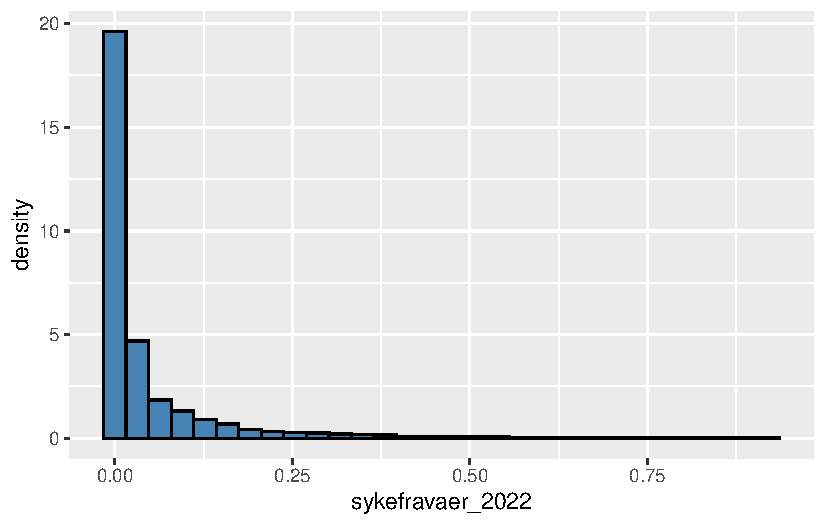
\includegraphics{kand_SOK2209_Bacheloroppgave_V25_files/figure-pdf/unnamed-chunk-9-1.pdf}

med de med 0, logtransformert med +0.01

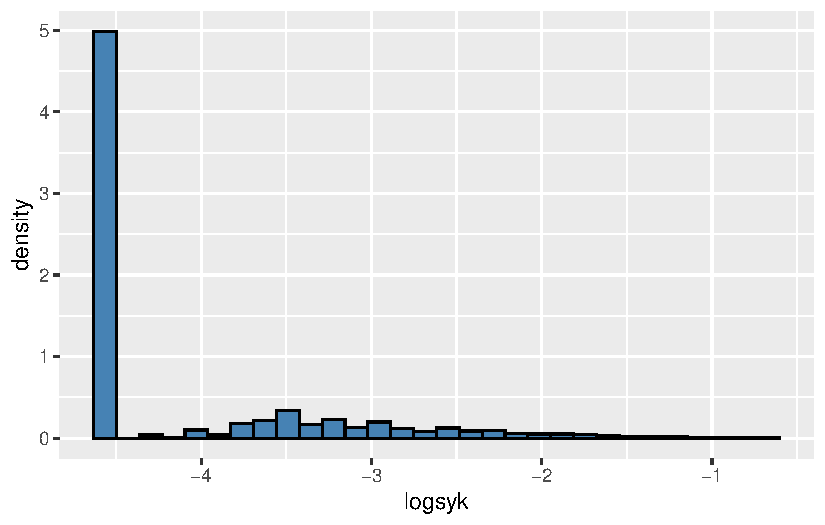
\includegraphics{kand_SOK2209_Bacheloroppgave_V25_files/figure-pdf/unnamed-chunk-10-1.pdf}

Uten de med 0 sykefravær, logtransformert.

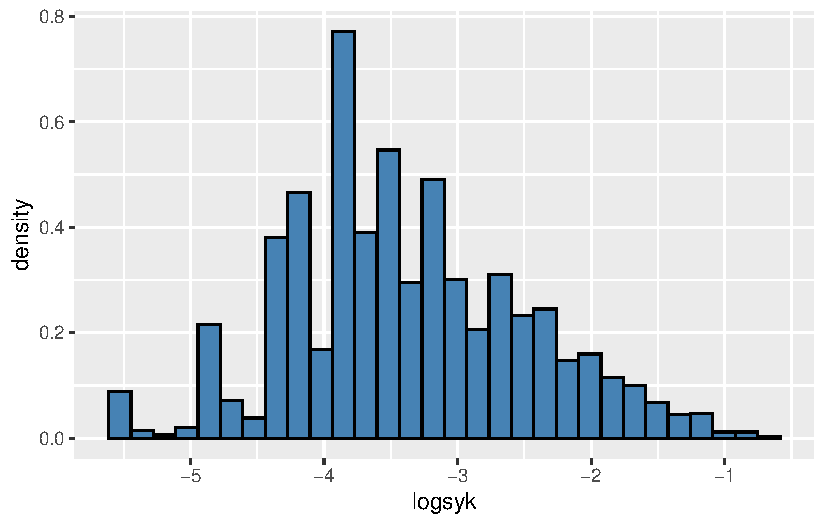
\includegraphics{kand_SOK2209_Bacheloroppgave_V25_files/figure-pdf/unnamed-chunk-11-1.pdf}

\begin{figure}[H]
\caption{Histogram og tetthetskurve for sykefravær i 2022}
\label{fig:histogram}
\centering
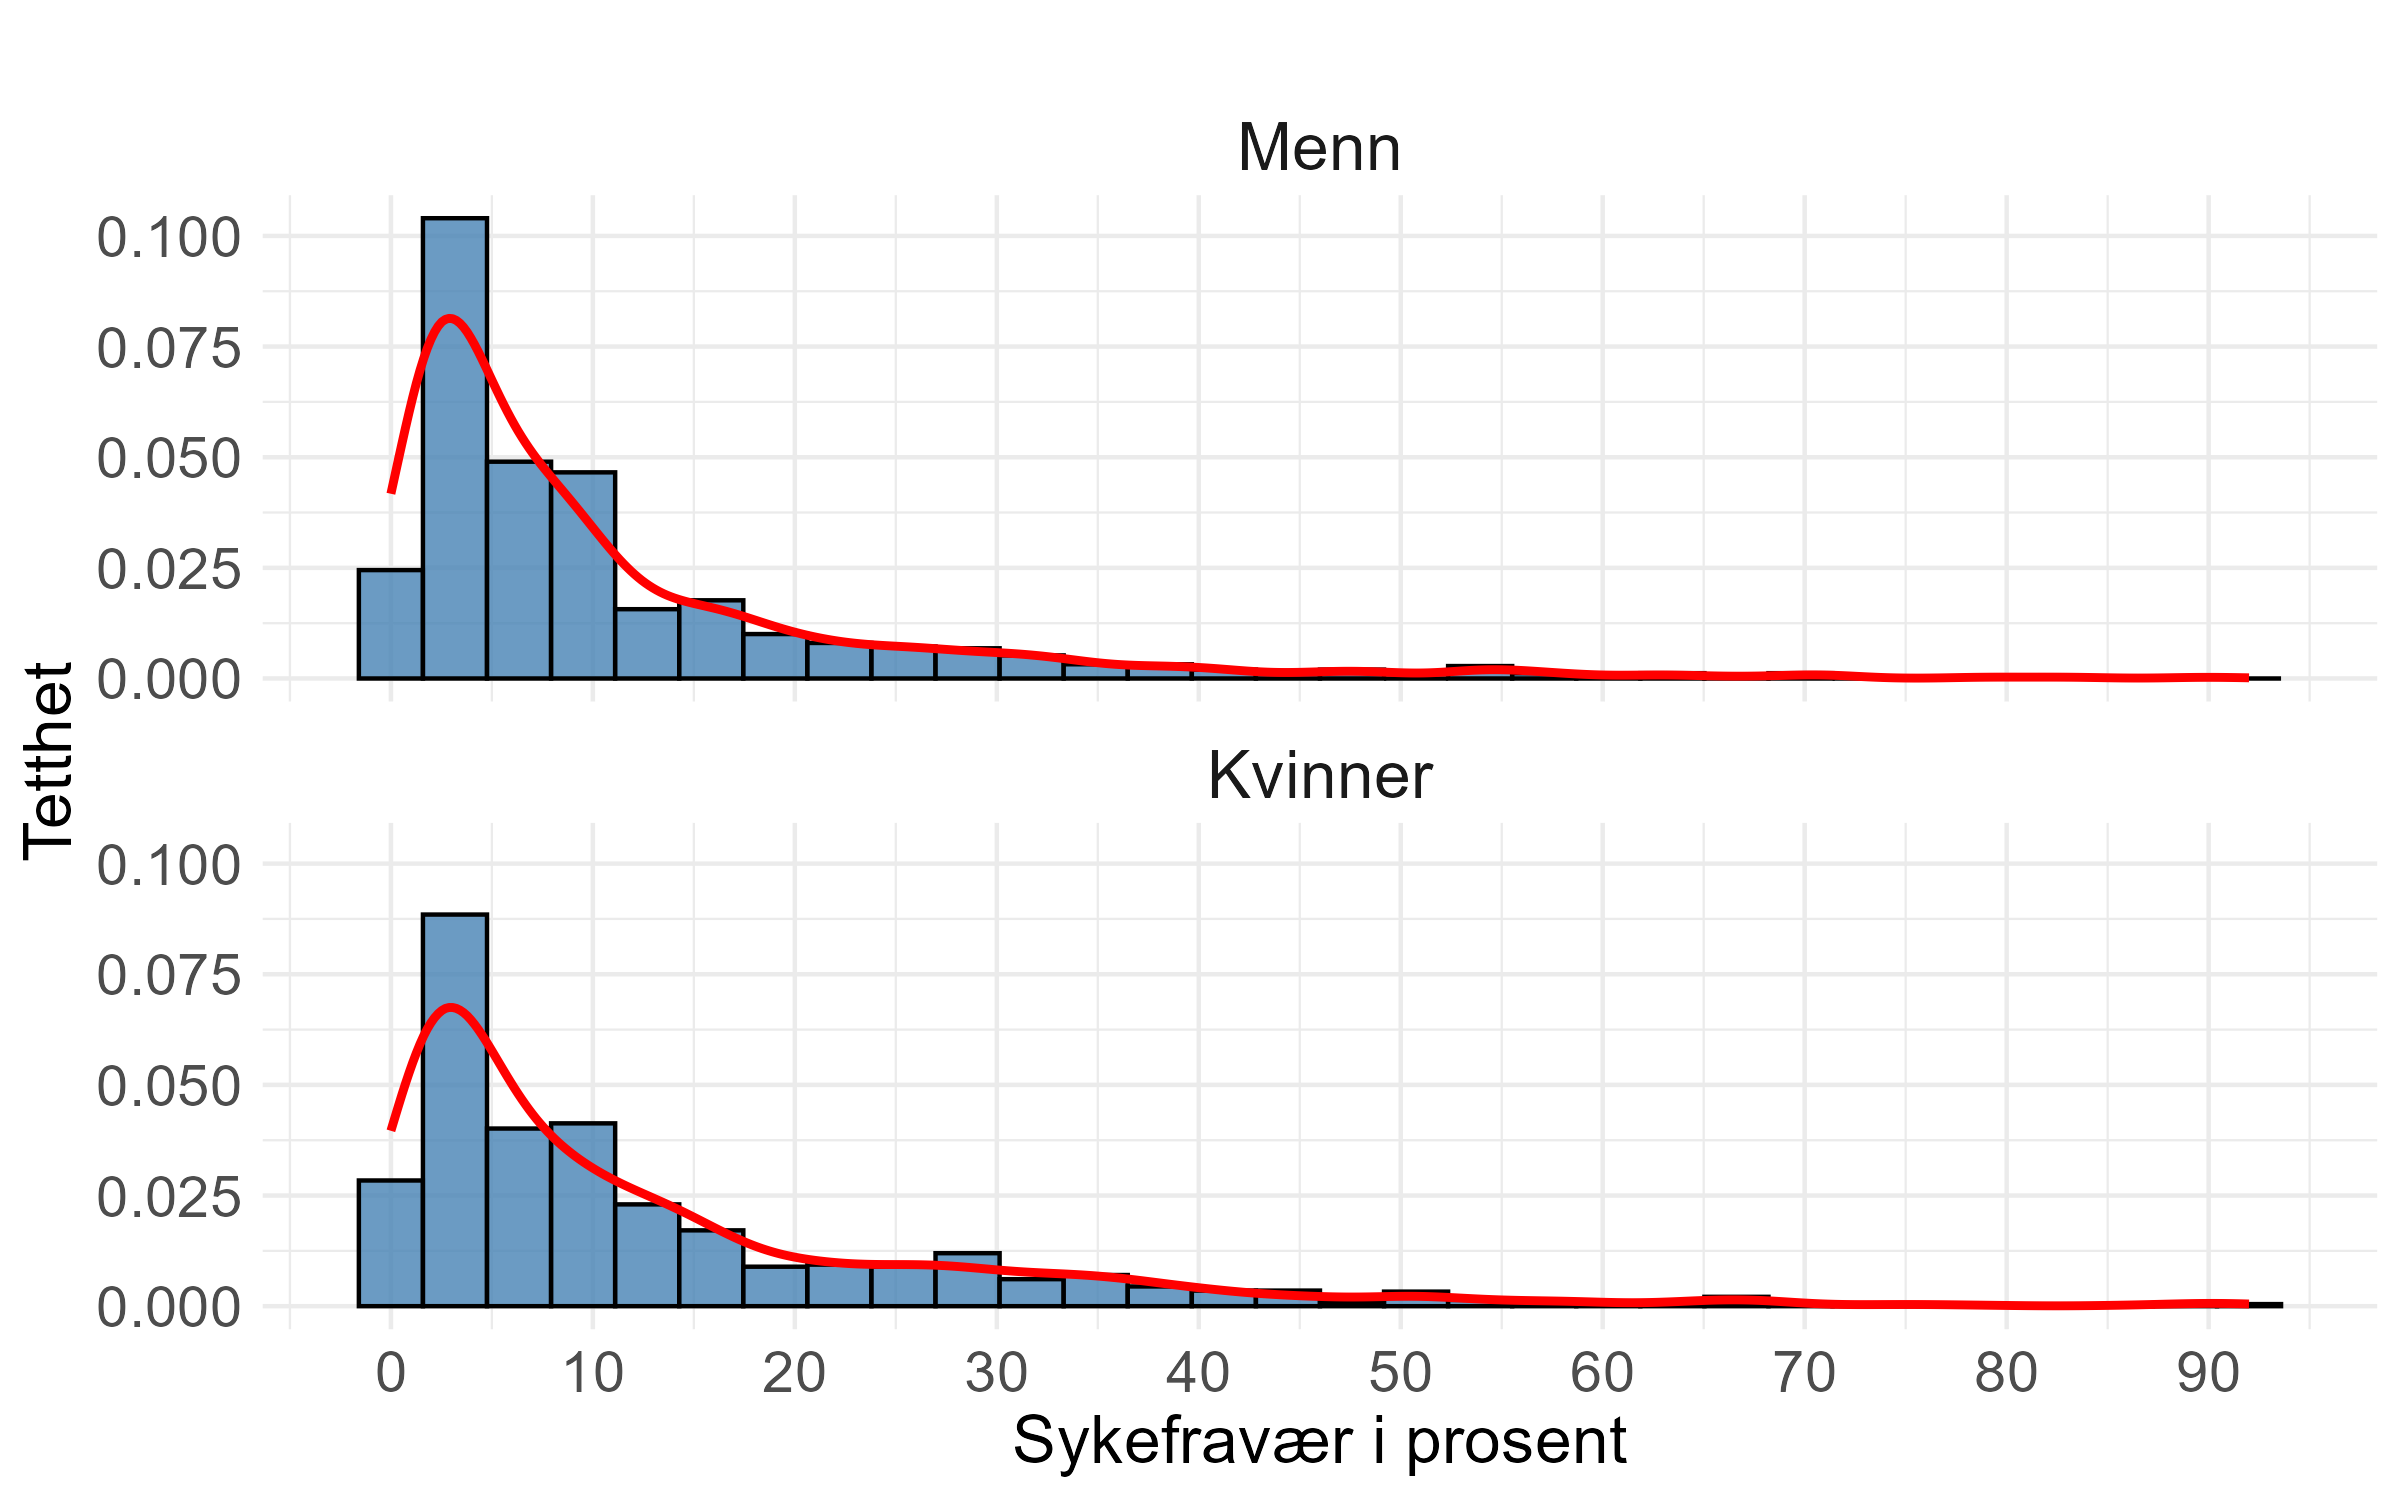
\includegraphics[width=0.8\textwidth]{dokumentobjekter/figurer/fig_1.png}
\end{figure}

Når vi ser på aldersfordelingen i \autoref{fig:histogram} så ser vi at
den er jevn og symmetrisk fordelt blant respondentene. Som nevnt
tidligere så er spennet på alderene til respondentene i undersøkelsen
mellom 18 til 66 år. Medianalderen kan man se i den blå stiplede linjen
som er på 43 år for menn og 44 år for kvinner.

\begin{figure}[H]
\caption{Histogram og tetthetskurve for alder}
\label{fig:histogram}
\centering
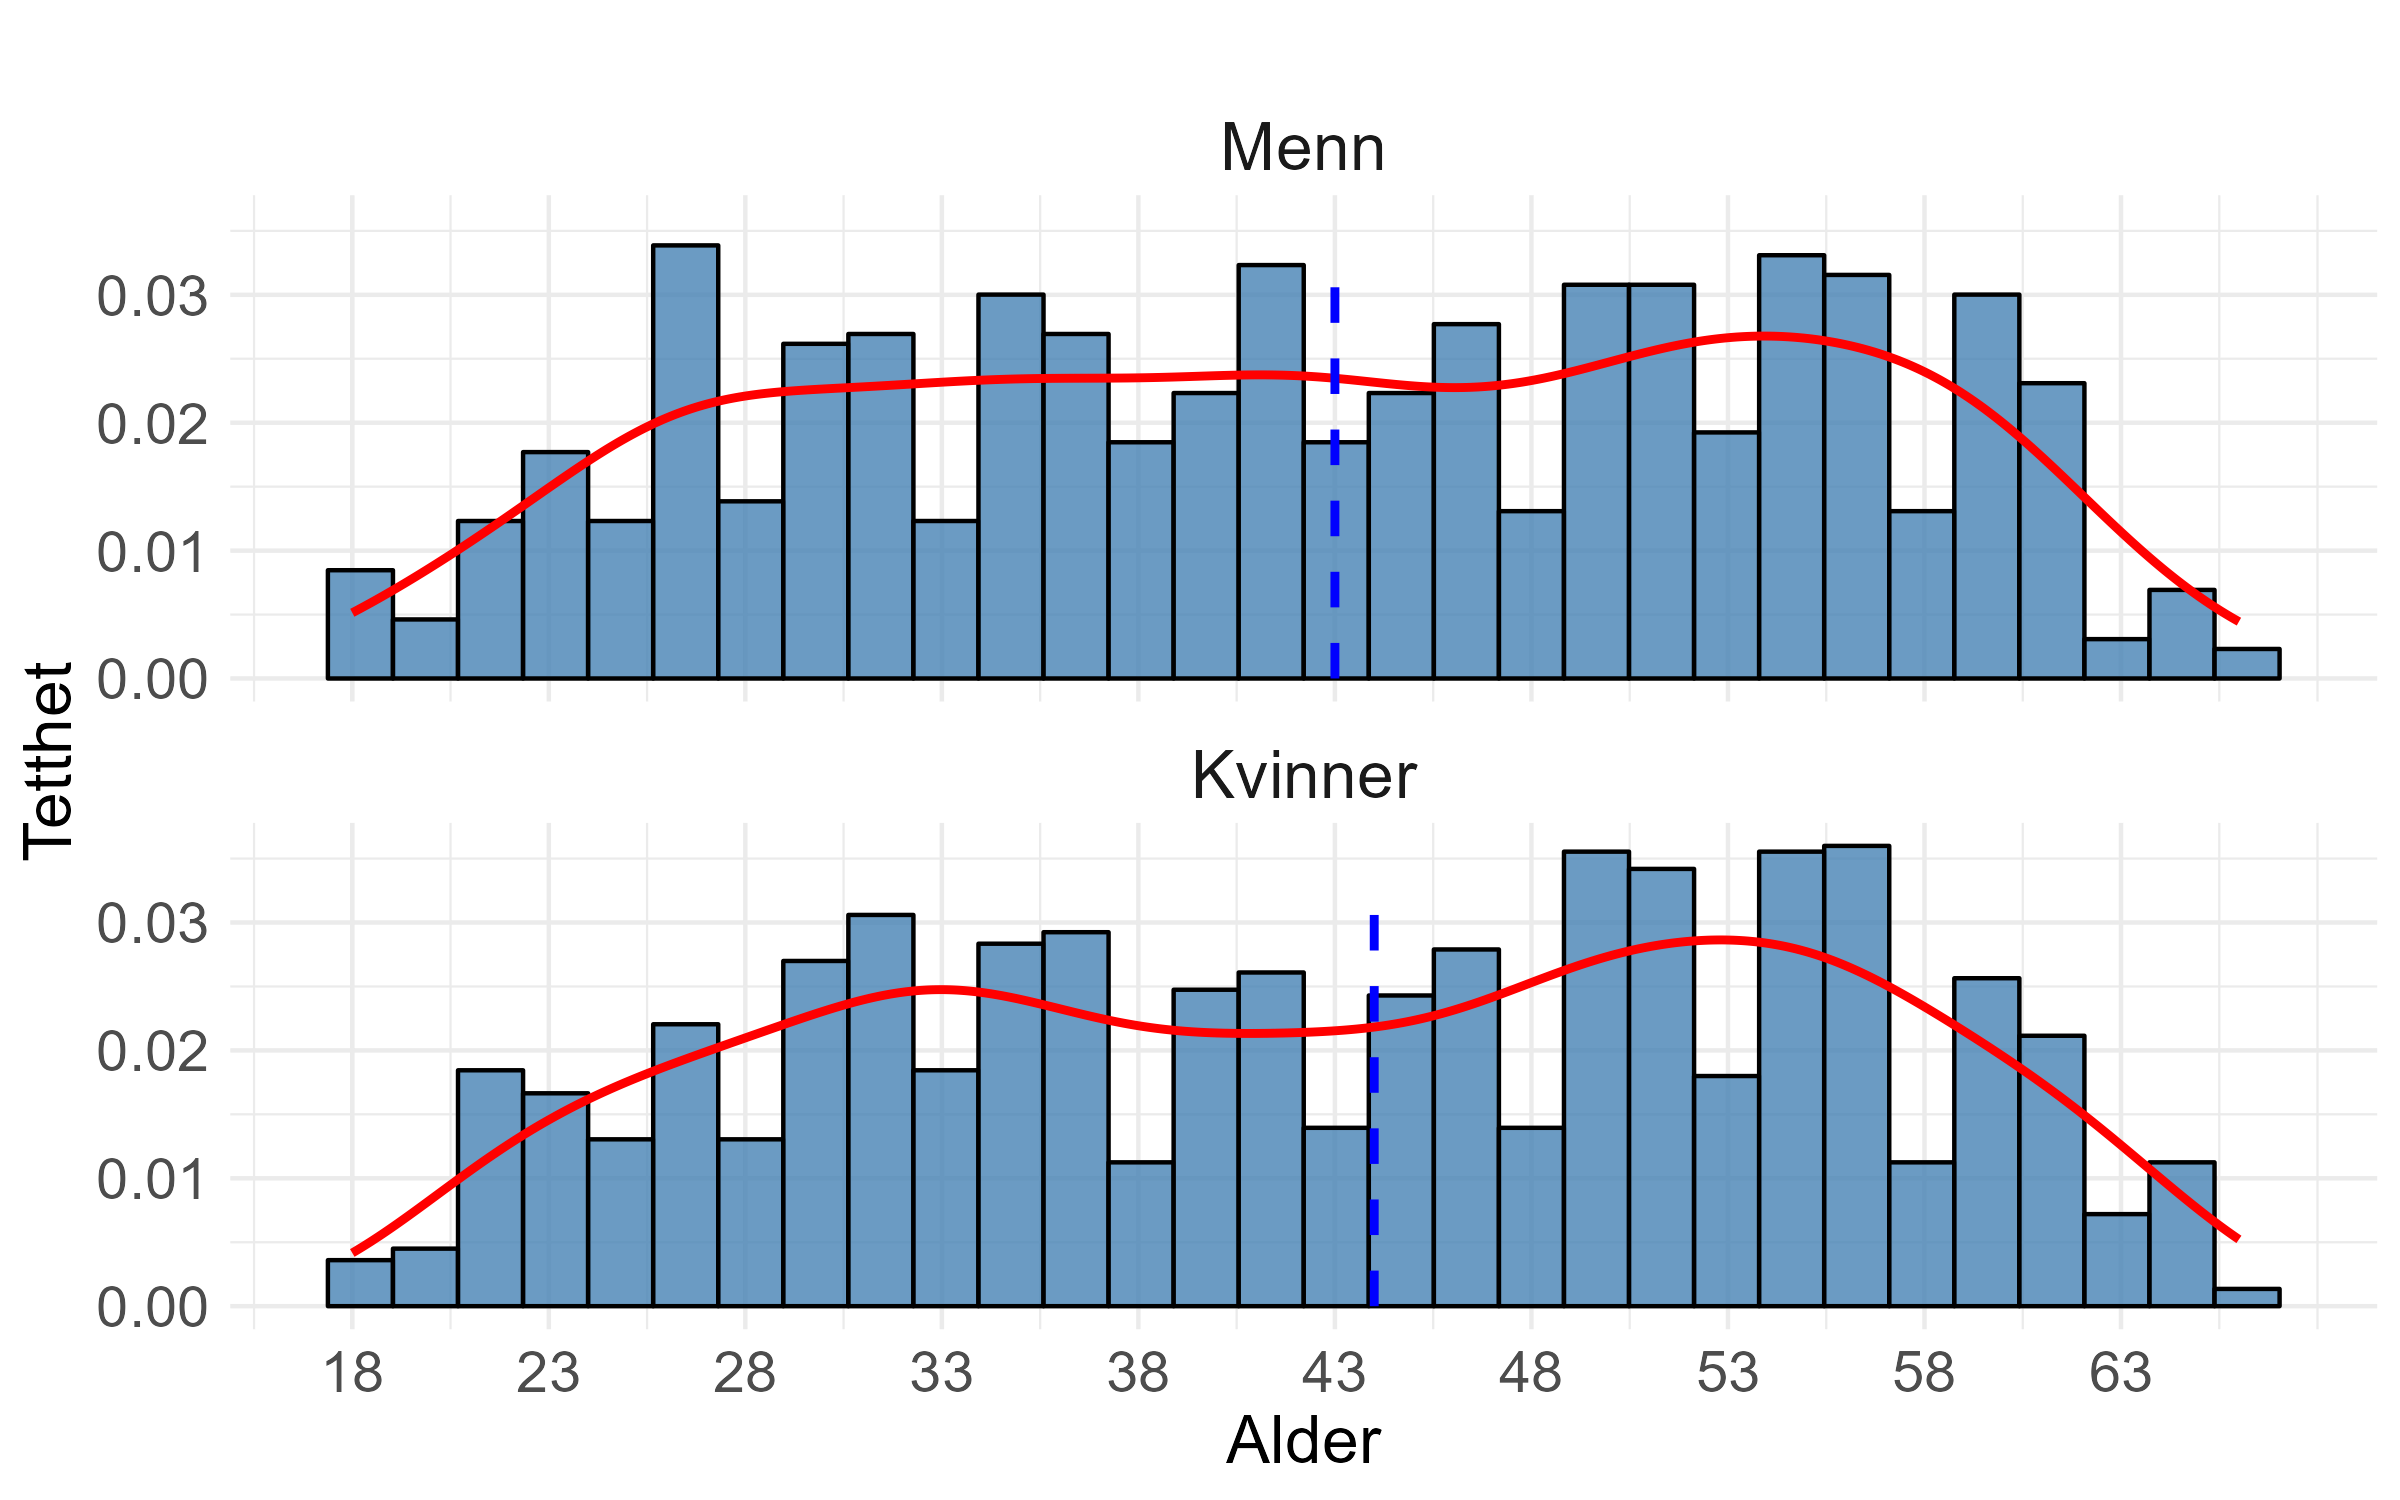
\includegraphics[width=0.8\textwidth]{dokumentobjekter/figurer/fig_2.png}
\end{figure}

For analysen så har vi fordelt alder inn i tre breddeintervaller på
18-29, 30-55 og 55-66 år. I \autoref{fig:barplot} presenteres et barplot
av aldersgruppene. Vi har flest respondenter i aldersgruppen 30-54 år
med 60.1 prosent som vi bruker som referansegruppe.

\begin{figure}[H]
\caption{Aldersgruppefordeling}
\label{fig:barplot}
\centering
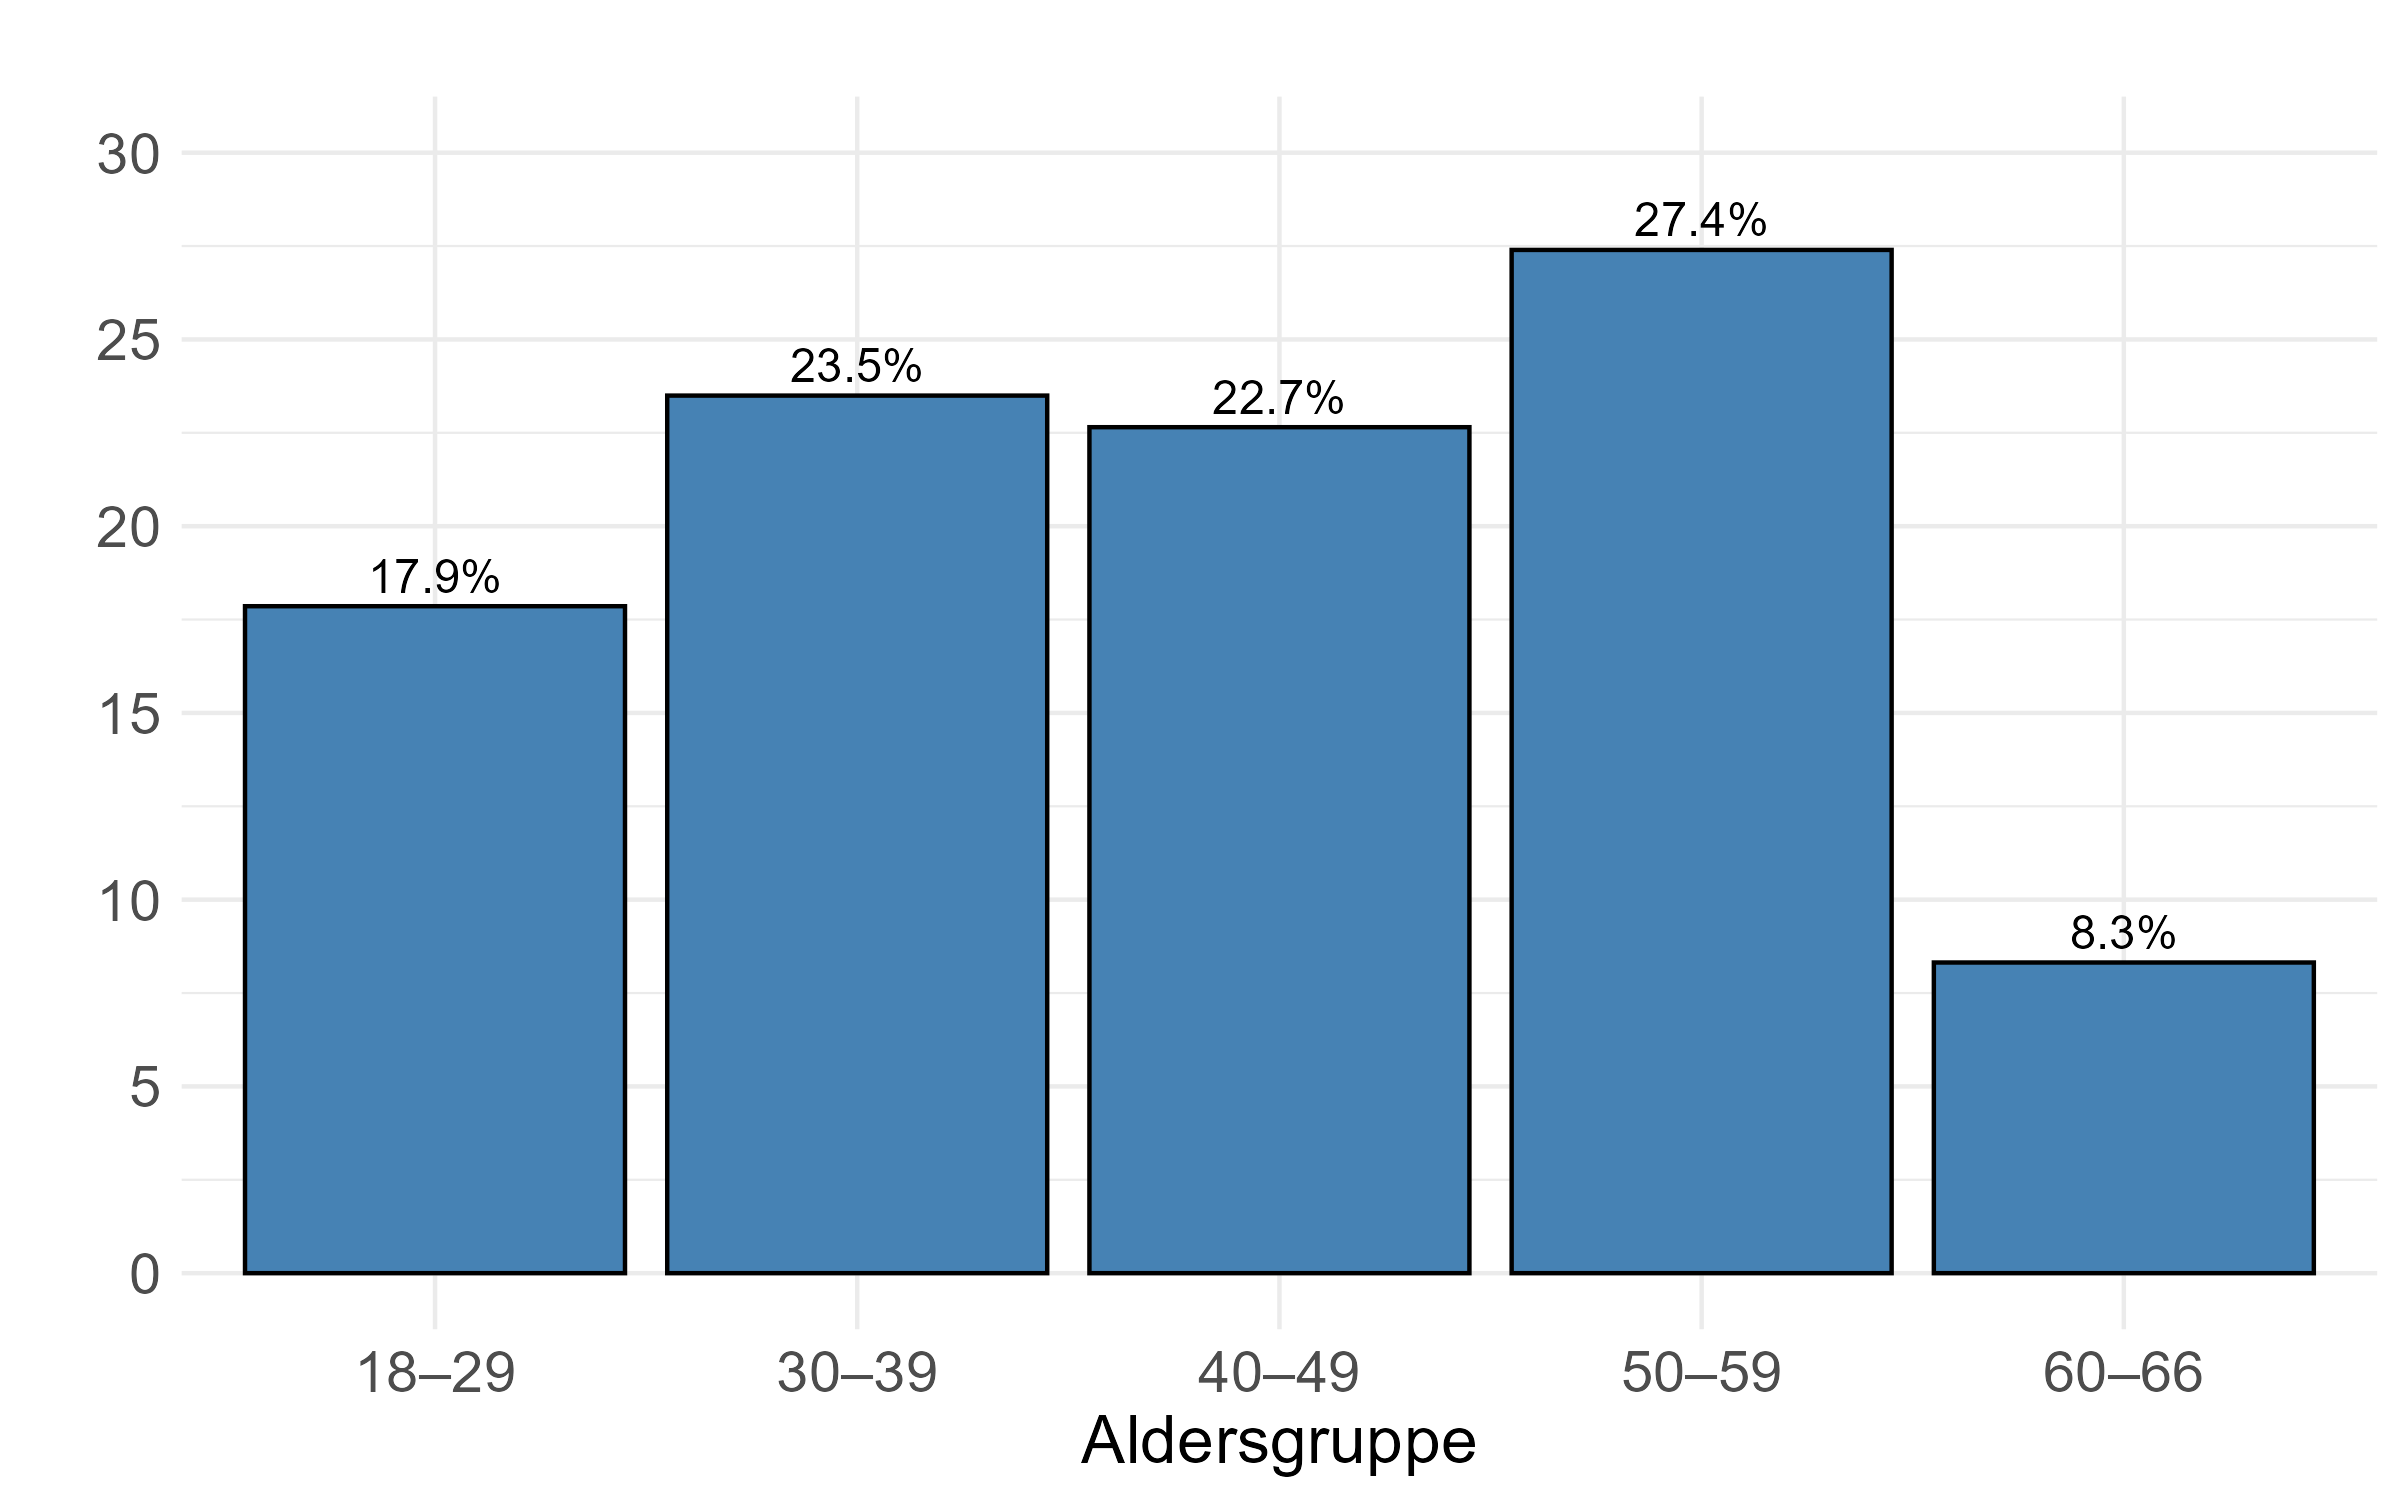
\includegraphics[width=0.8\textwidth]{dokumentobjekter/figurer/fig_3.png}
\end{figure}

\clearpage

\begin{wrapfigure}{r}{0.5\textwidth} 
    \centering
    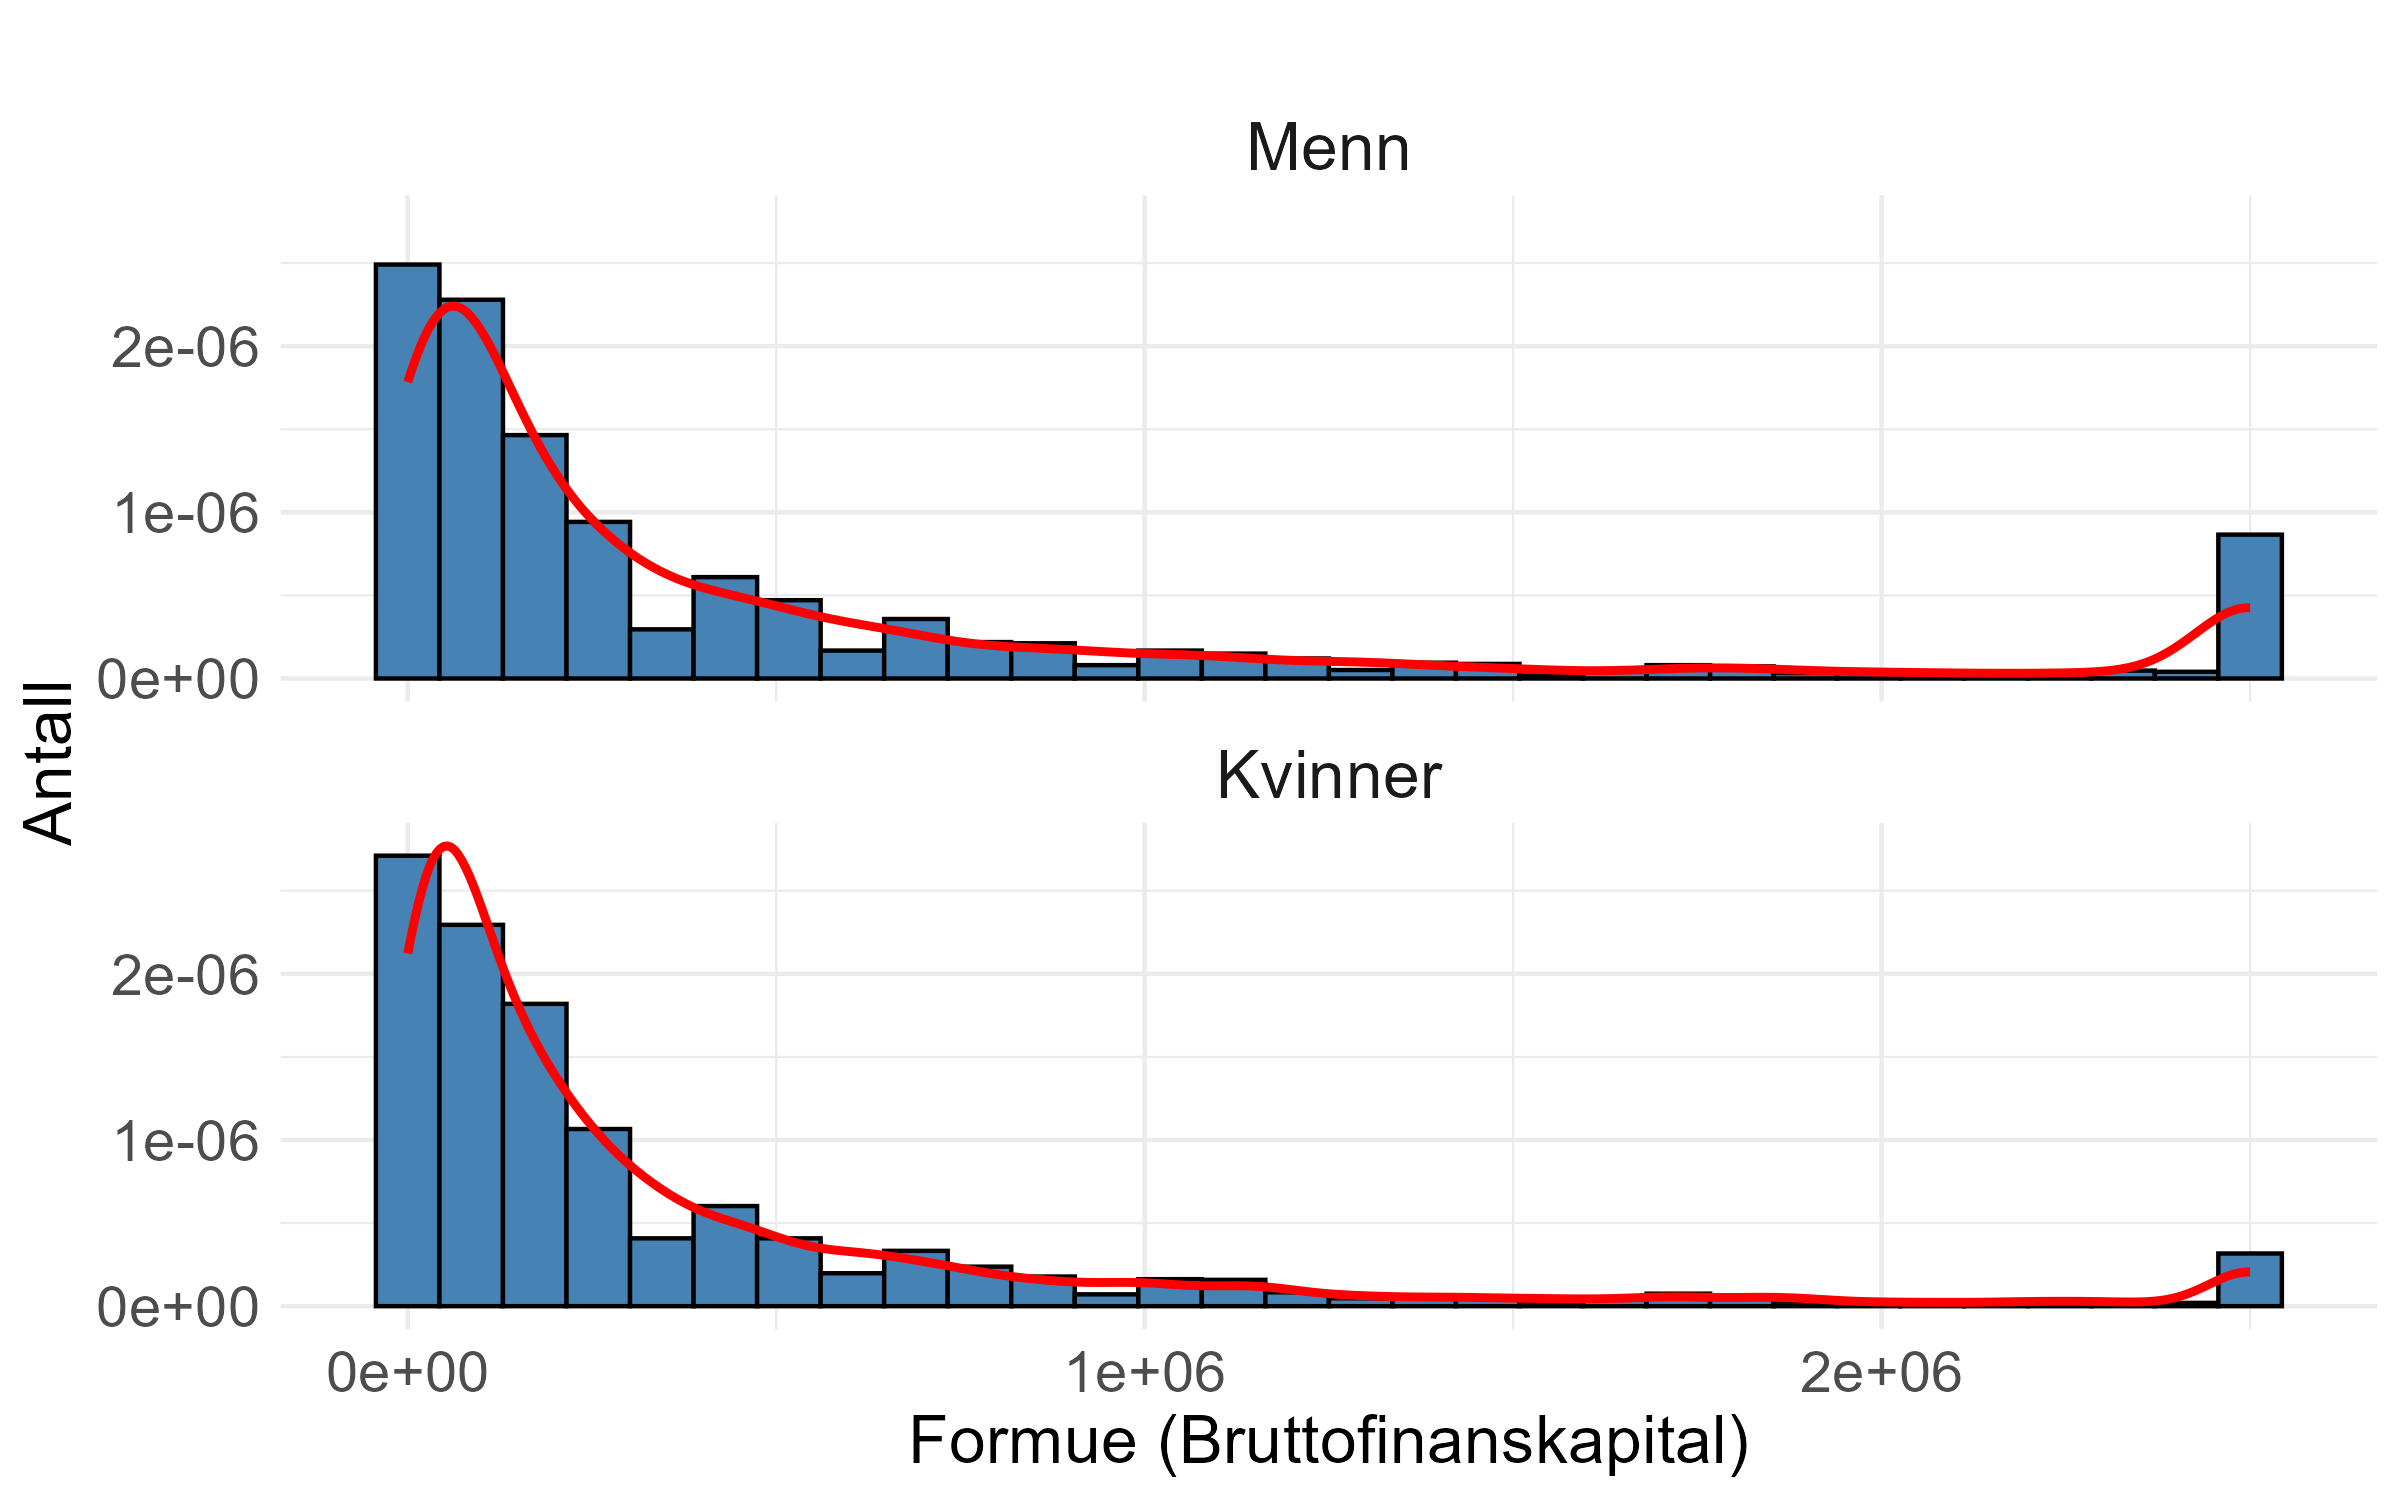
\includegraphics[width=0.5\textwidth]{dokumentobjekter/figurer/fig_4_1.png}
    \caption{Fordeling av bruttofinanskapital}
    \label{fig:histogram_formue}
    \smallskip\par
    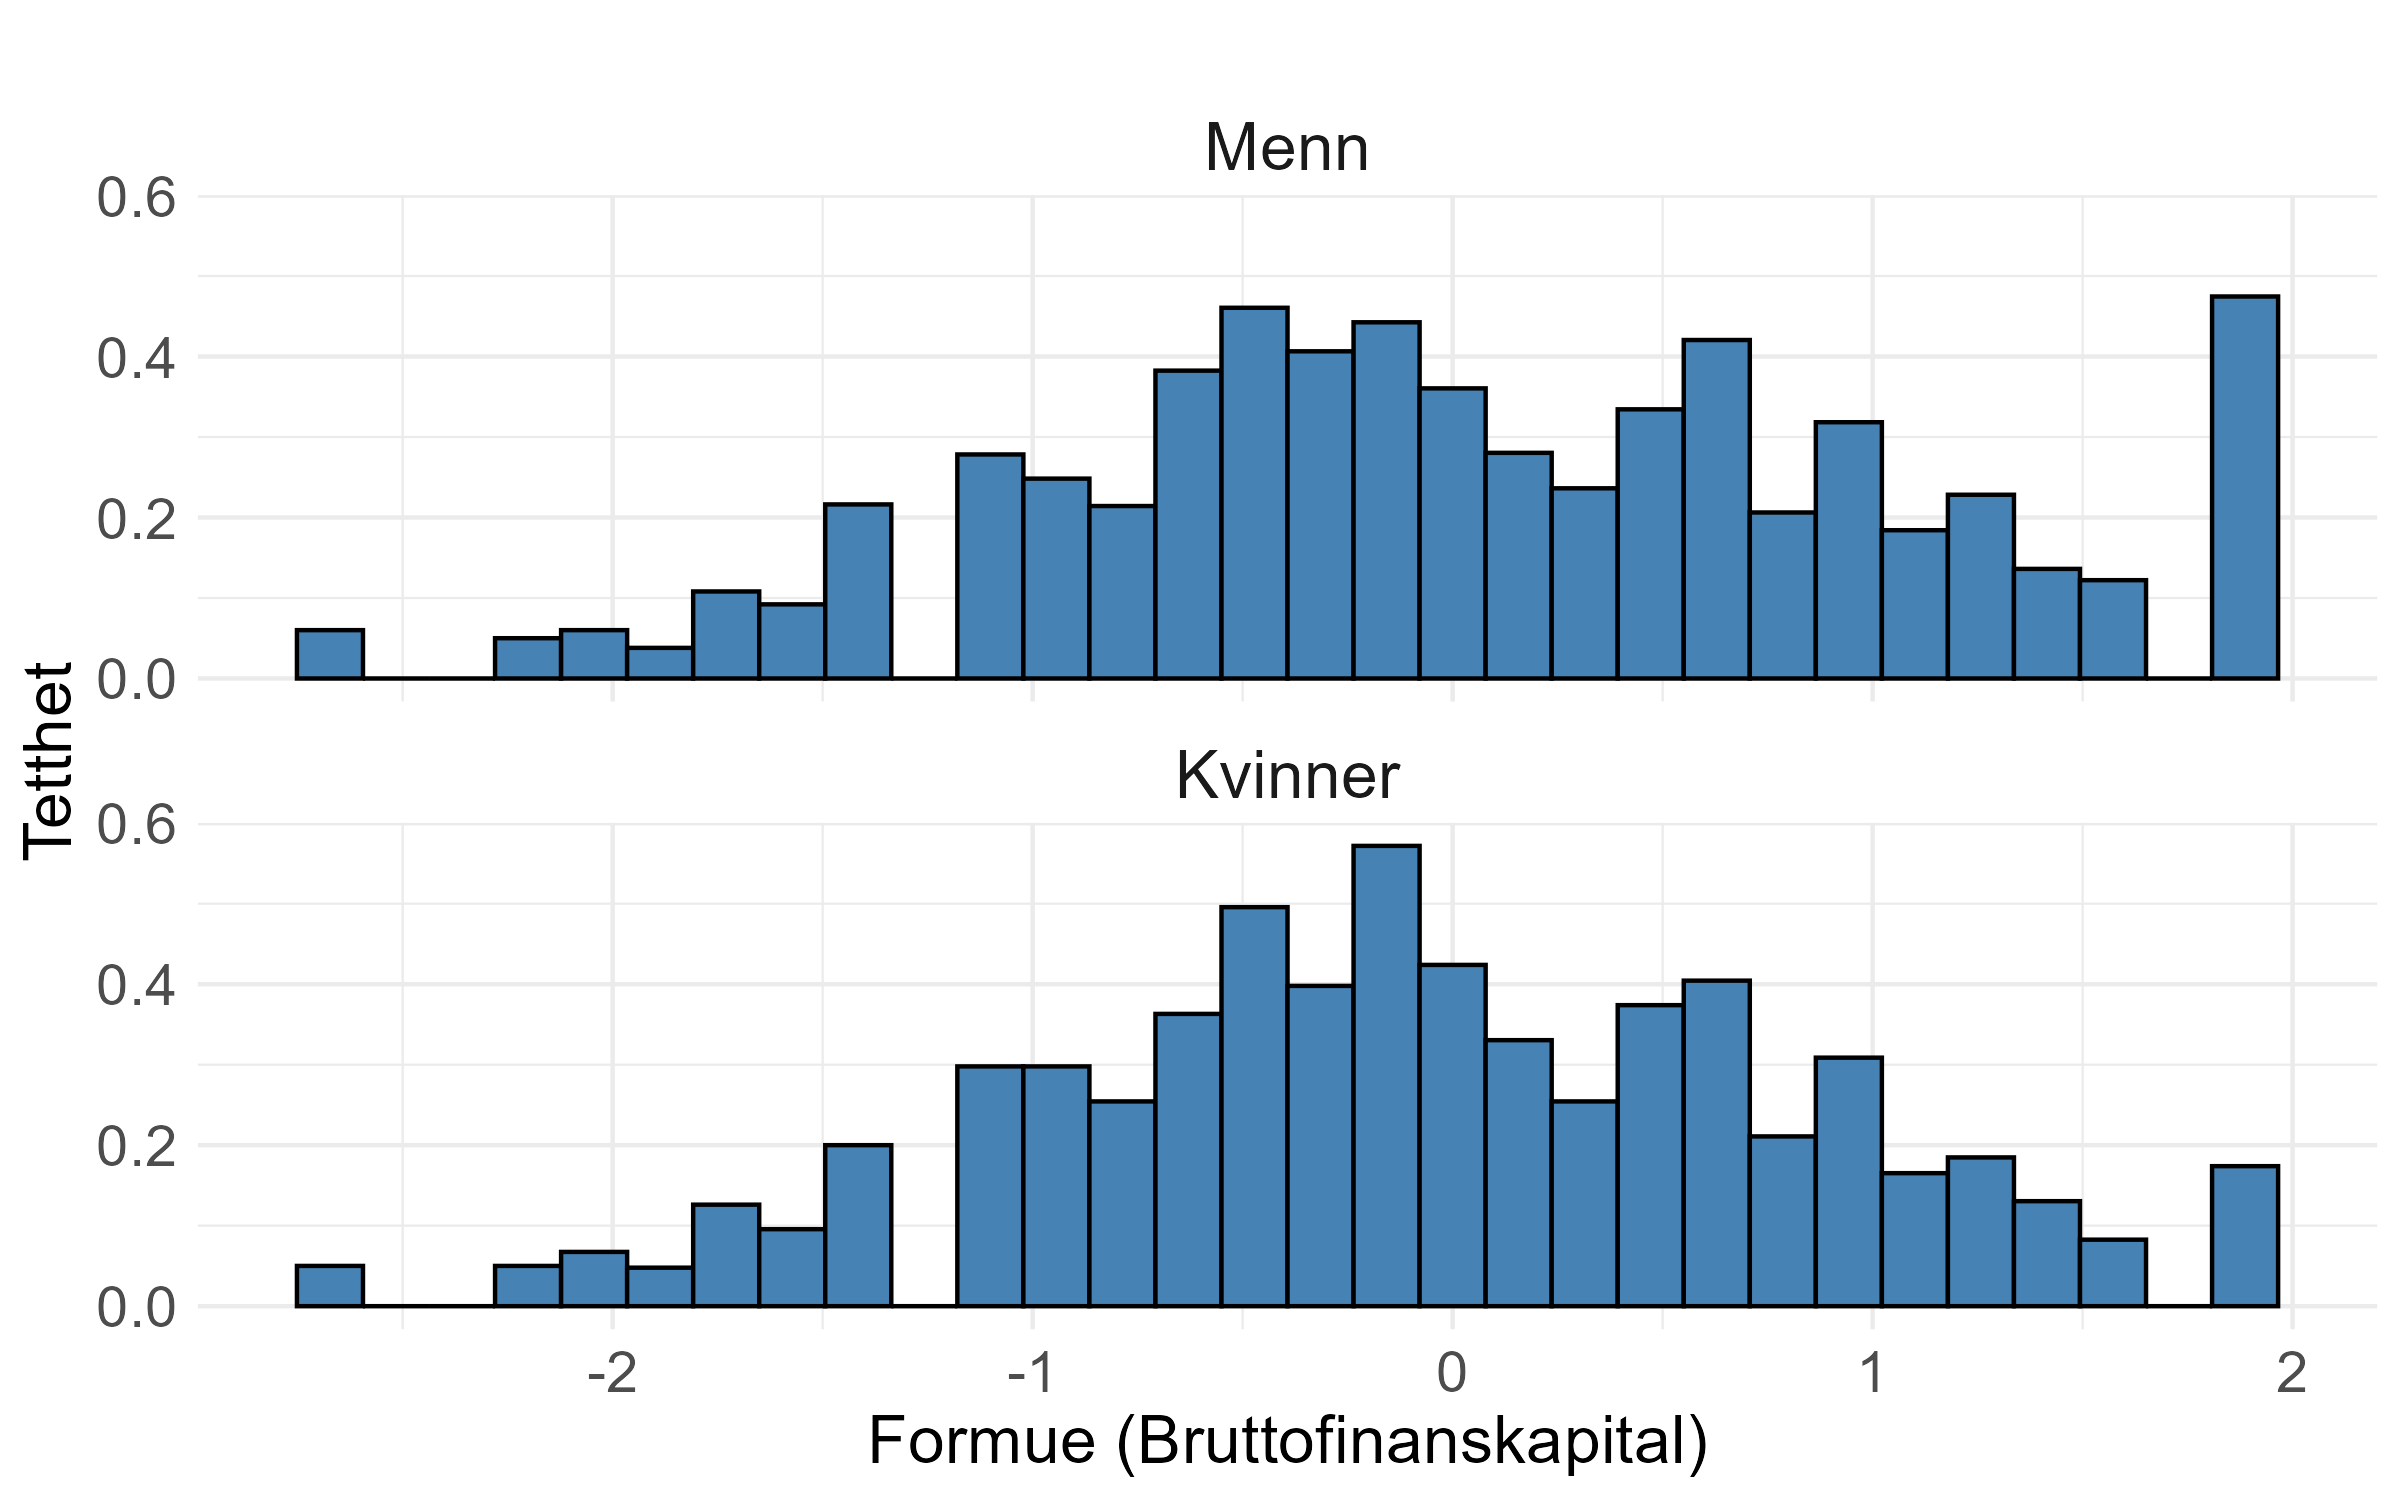
\includegraphics[width=0.5\textwidth]{dokumentobjekter/figurer/fig_4_2.png}
    \caption{Invertert kumulativ fordeling av bruttofinanskapital}
    \label{fig:histogram_formue_fordeling}
\end{wrapfigure}

\#måfiks I \autoref{fig:histogram_formue} presenteres histogram og
tetthetskurve for bruttofinanskapitalen log-transformert \((1 + x)\)
{[}\^{}8{]}. Originalt er formuefordelingen høyreskjev, med en høyere
andel av respondentene som har lav formue enn de som har høy formue noe
som kan svekke analysen. Derfor må vi log-transformere formuefordelingen
for å få en mer normalfordelt fordeling både for menn og kvinner. Når
man log-transformerer \((1 + x)\) så tar vi logaritmen av formueverdiene
og legger til 1 for å unngå problemer med nullverdier.

Vi har da \(n_{lav} = 1160\), \(n_{middels} = 5172\) og
\(n_{høy} = 1166\). Den laveste gruppen har formue fra \(0 - 30000\),
den middels gruppen har formue fra \(30000 - 850000\) og den høyeste
gruppen har formue fra \(850000 - 2500000\). Dette gir oss en god
fordeling av formuegruppene, og vi kan se om det er forskjeller i
sykefravær mellom de forskjellige gruppene.

\newpage

Når vi ser på fordelingen av formue- og utdanningsgrupper fordelt på
kjønn i \autoref{fig:barplot_2} så ser vi at det er flest kvinner i
utdanningsgruppen videregående skole med 46.7 prosent, og det samme
gjelder for menn med 56.9 prosent. Mer kvinner enn menn har
universitetsutdannings eller høyere med 40.2 prosent mot kun 18.5
prosent for menn. Menn har også lavest utdanningsnivå med 24.6 prosent i
utdanningsgruppen grunnskole eller mindre, mens kvinner har 13.1 prosent
i den samme utdanningsgruppen. Dette viser oss at menn har lavere
utdanningsnivå enn kvinner, og at kvinner er mer tilbøyelige til å ta
høyere utdanning enn menn.

\#MÅfiks Formuefordelingen er delt inn i tertiler, som gjør slik at
fordelingen blir jevnt blant de forskjellige formuegruppene både for
menn og kvinner.

\begin{figure}[H]
\caption{Fordeling av formue- og utdanningsgrupper fordelt på kjønn}
\label{fig:barplot_2}
\centering
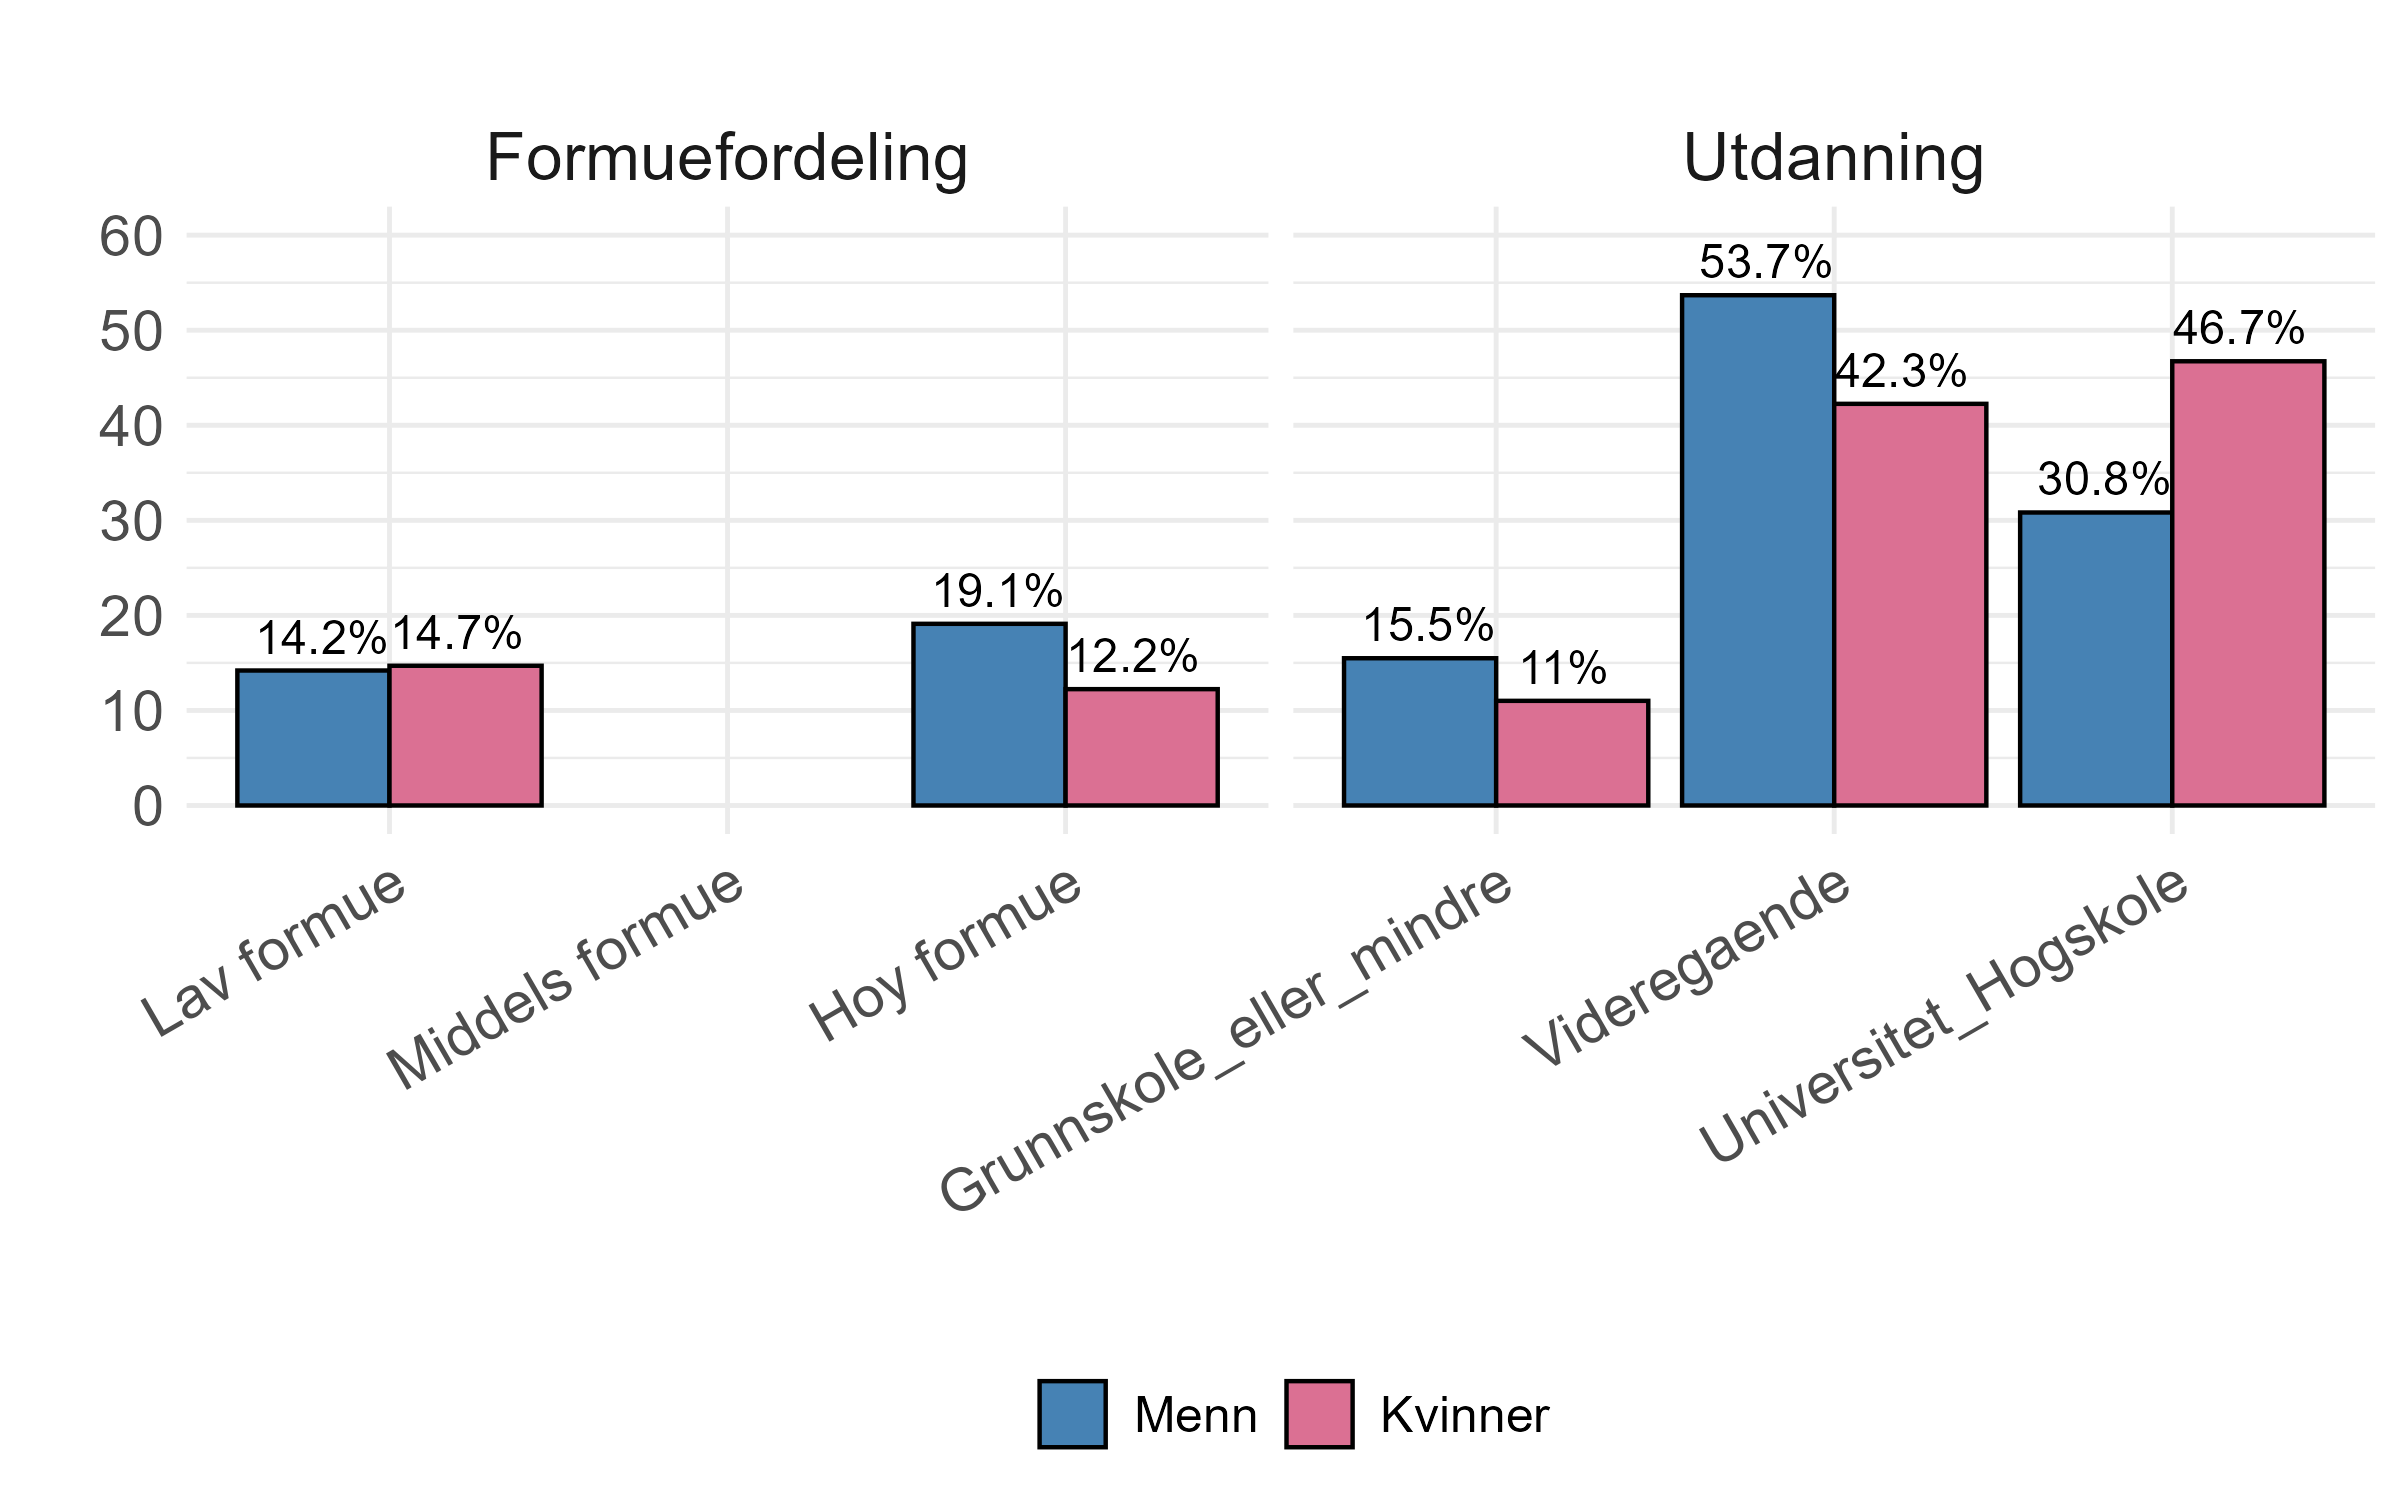
\includegraphics[width=0.8\textwidth]{dokumentobjekter/figurer/fig_5.png}
\end{figure}

I \autoref{fig:boxplot} presenteres et boksplott av sykefravær etter
formuegruppe. Vi kan se at det ikke er store forskjeller i sykefraværet
mellom formuegruppene. Medianen vises i den sorte streken i midten av
boksen, og den viser at sykefraværet med små marginer går ned fra lav
formue, til middels formue og til høy formue. Bunnen og toppen til
boksene viser oss henholdsvis første og tredje kvartil, og de stiplede
linjene viser oss minimum og maksimum sykefravær. Det er også noen
uteliggere som er vist med små prikker, og de viser at det er noen
respondenter som har rapportert sykefravær på over 40 prosent. Dette kan
være at de har vært sykemeldt i en lengre periode. I bakgrunnen av
figuren man man se alle observasjonene spredt utover for en bedre
oversikt siden det er mange observasjoner som går over hverandre i
boksen. Dette er gjort med en funksjon som sprer ut observasjonene litt
for å få en bedre oversikt over dem.

\begin{figure}[H]
\caption{Boksplott av sykefravær etter formuegruppe}
\label{fig:boxplot}
\centering
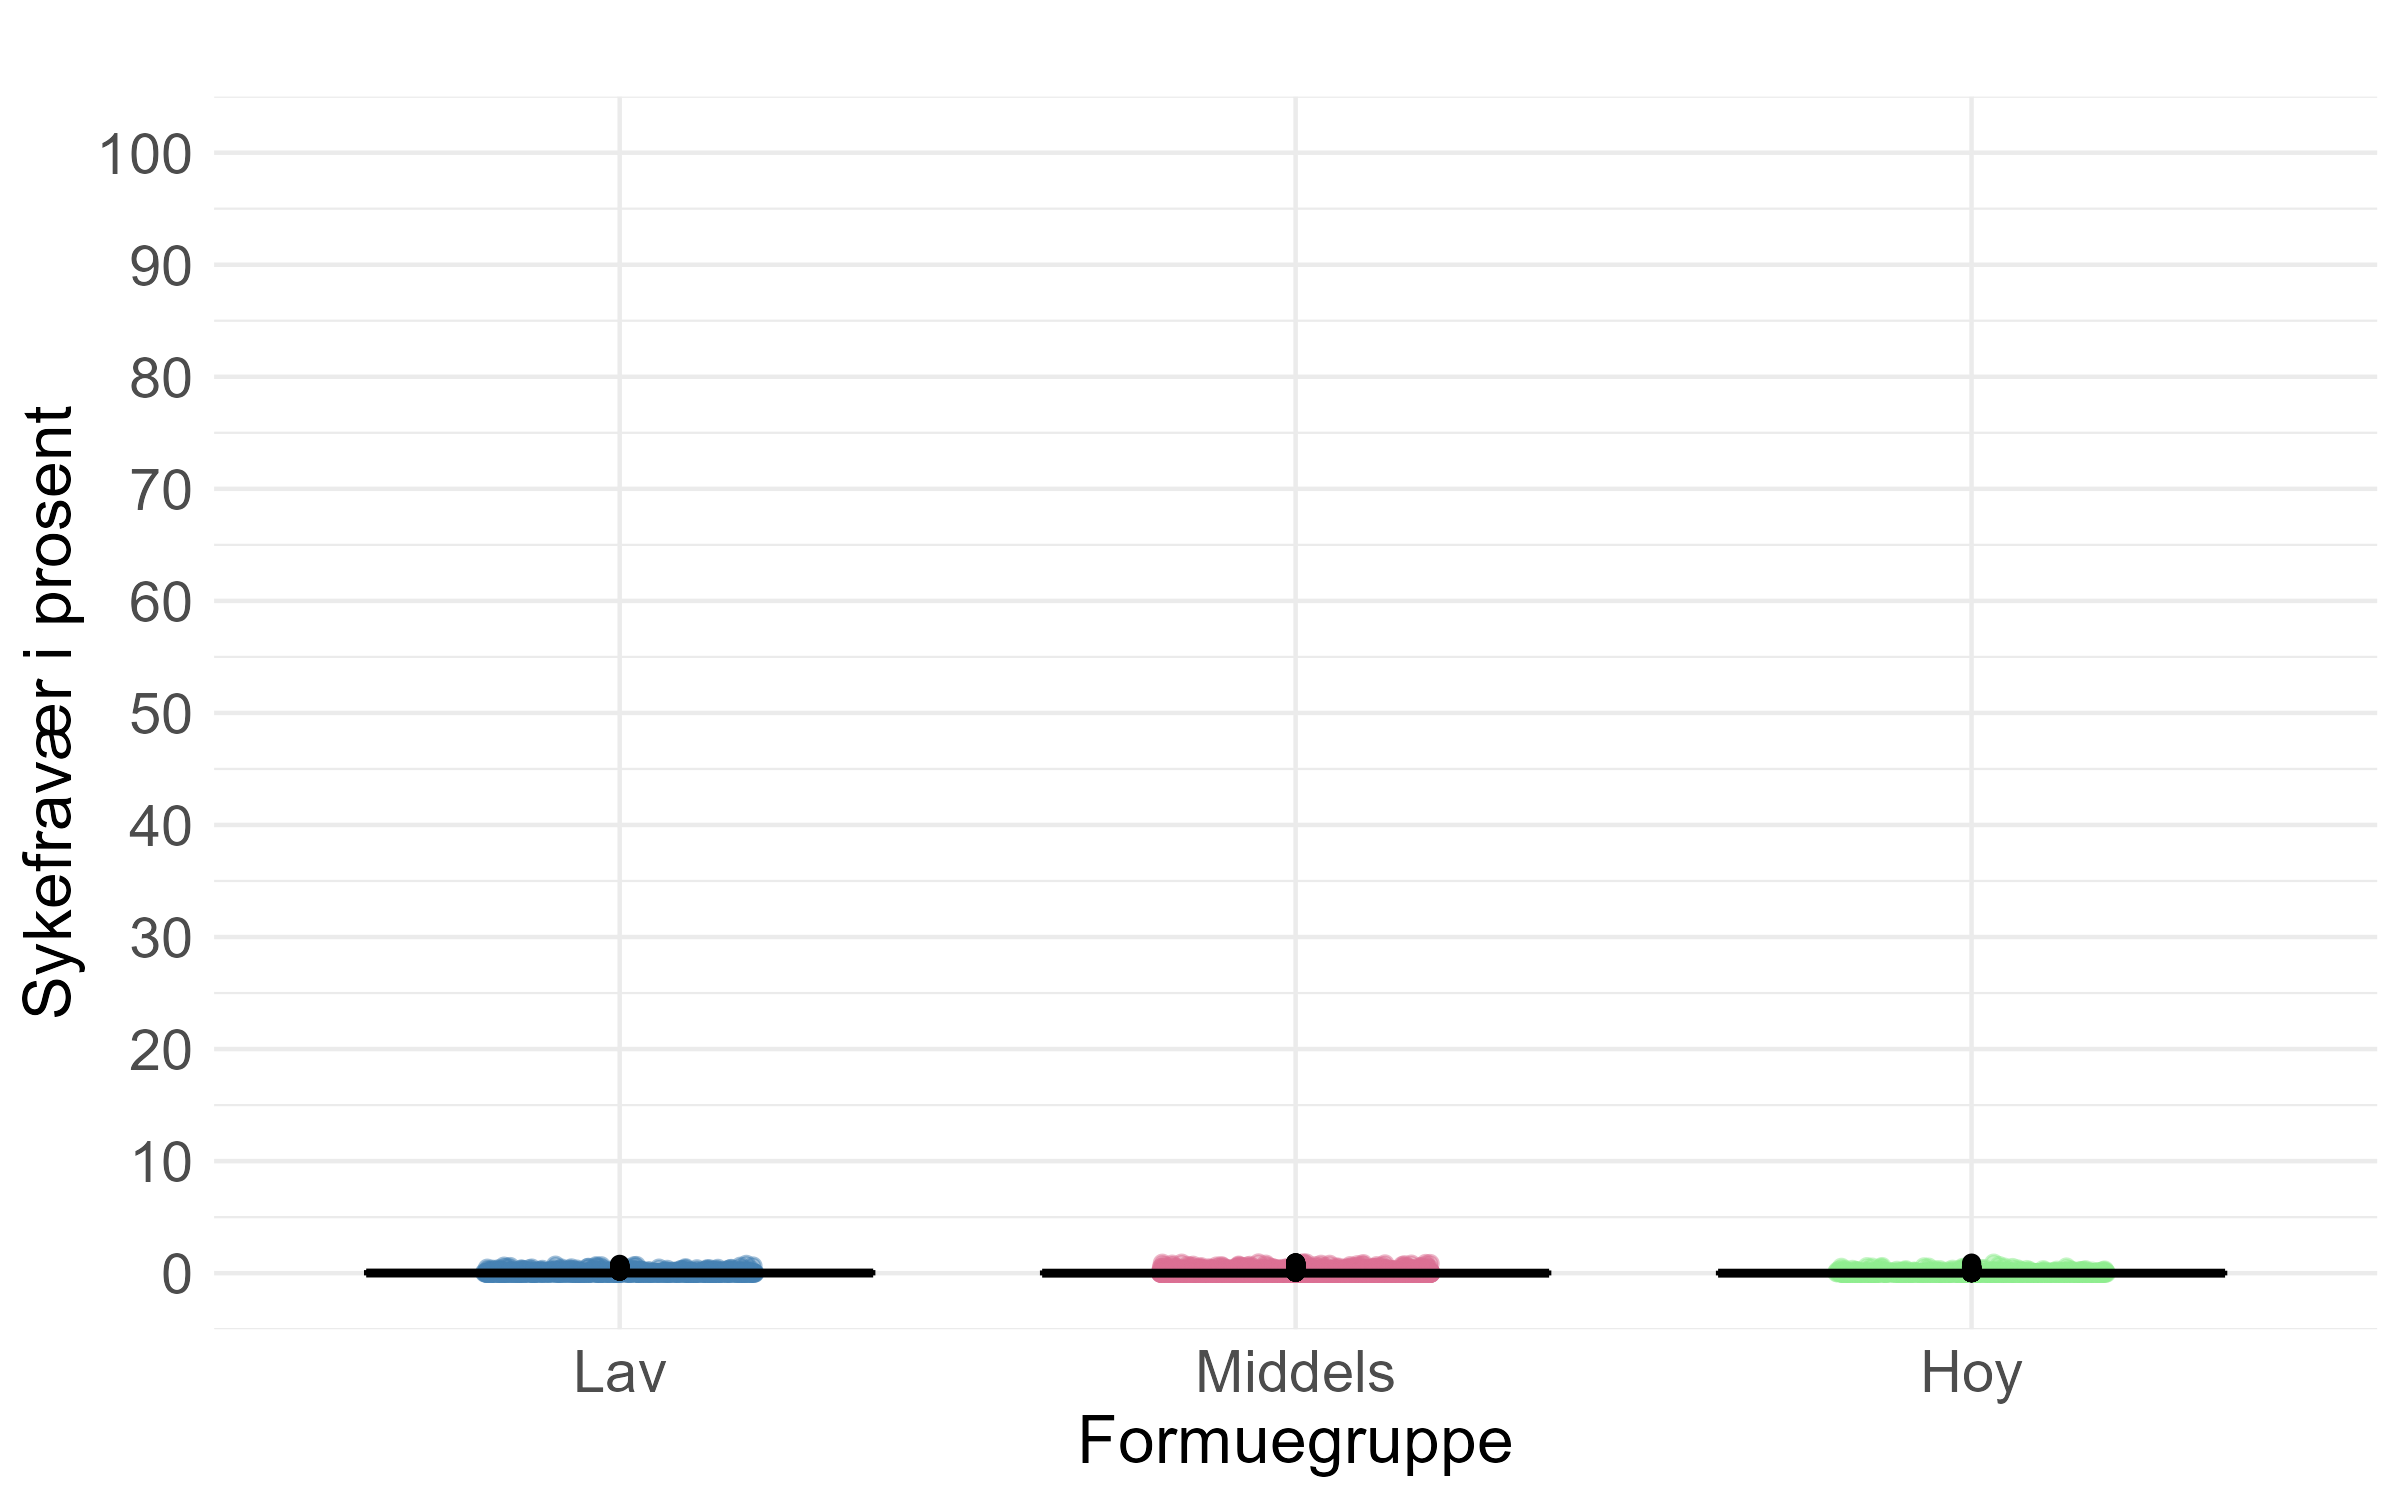
\includegraphics[width=0.8\textwidth]{dokumentobjekter/figurer/fig_6.png}
\end{figure}

I \autoref{fig:boxplot_2} presenteres et boksplott av sykefravær etter
utdanningsnivå. Vi ser at sykefraværet er veldig jevnt mellom
utdanningsnivåene. Medianen er litt over 10 prosent, og som tidligere
vet vi at gjennomsnittlig sykefravær er lavere for høyt utdannede og
litt lavere for de med lavere utdanning.

\begin{figure}[H]
\caption{Boksplott av sykefravær etter utdanningsnivå}
\label{fig:boxplot_2}
\centering
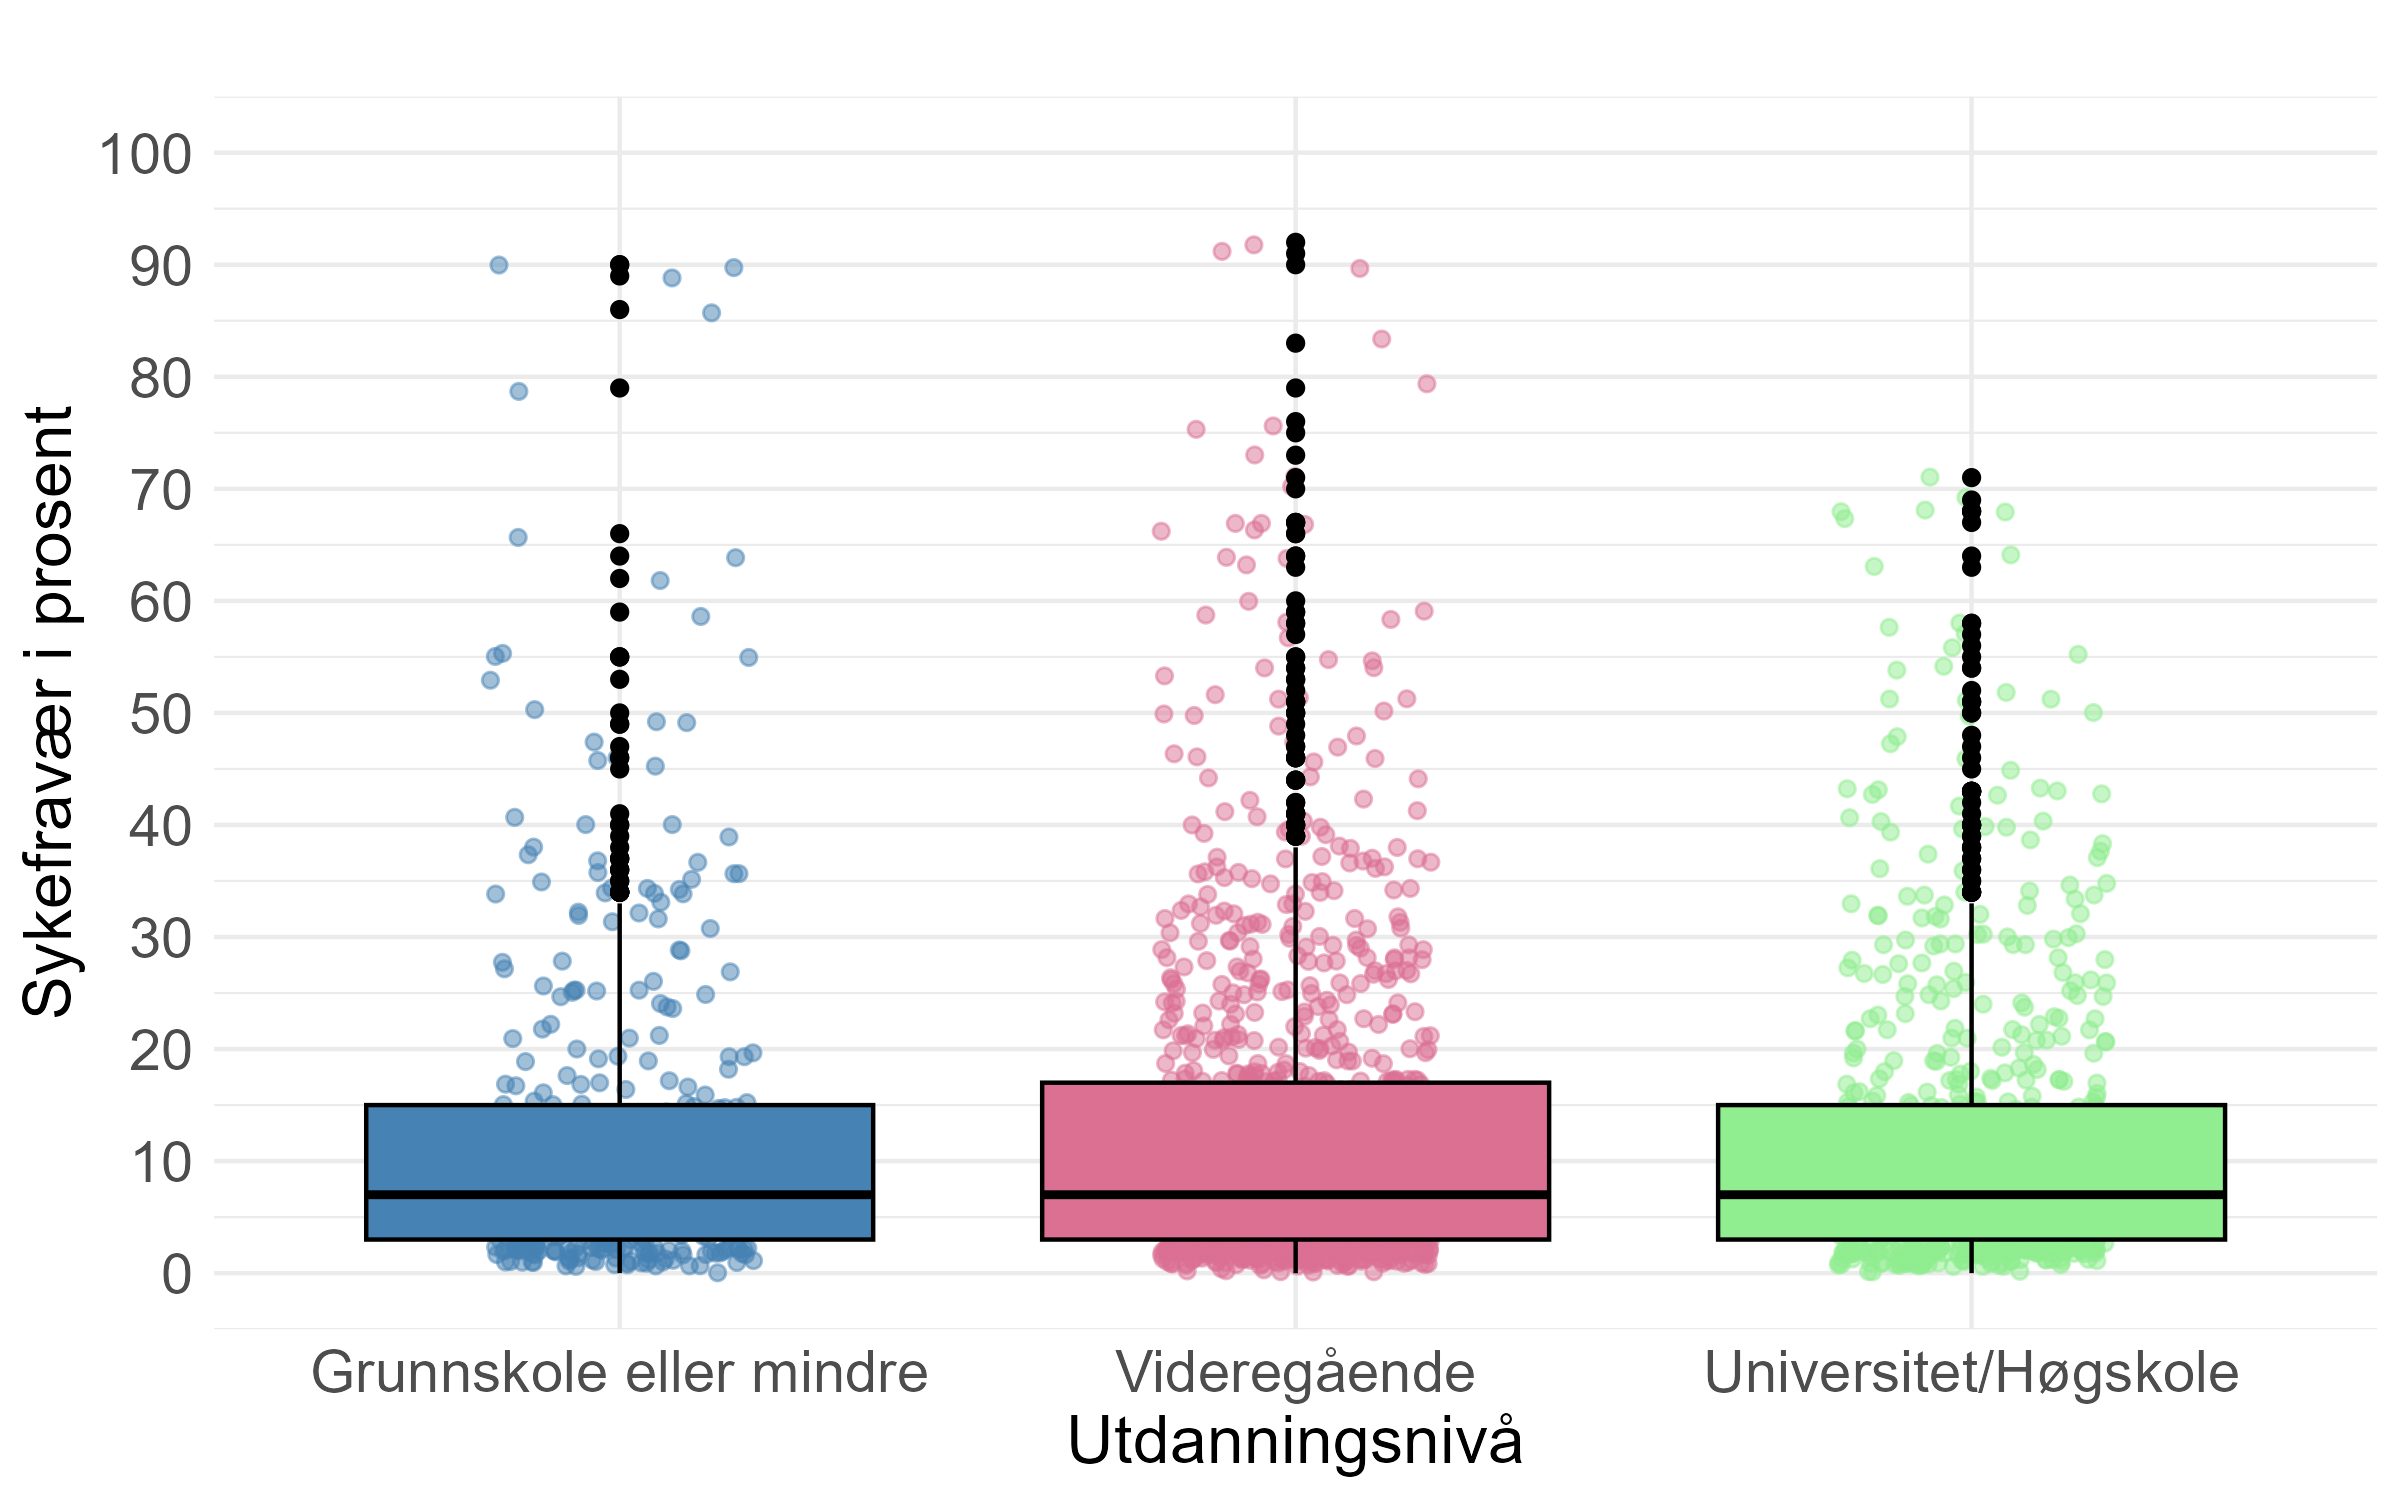
\includegraphics[width=0.8\textwidth]{dokumentobjekter/figurer/fig_7.png}
\end{figure}

Korrelationheatmap om vi får tid her til latente variabler.

\subsection{Metode \{sec-metode\}}\label{metode-sec-metode}

I oppgaven vil vi bruke en kvantitativ metode for å analysere
sammenhengen mellom formue og sykefravær. Vi vil bruke en Structural
Equation Model (SEM) for å teste hypotesene våre, og vi vil kontrollere
for andre relevante faktorer som kan påvirke sykefraværet. SEM er en
statistisk metode som gjør det mulig å teste komplekse modeller med
flere variabler, og som kan håndtere både direkte og indirekte
sammenhenger mellom variablene. Vi vil bruke R for å gjennomføre
analysen, og vi vil bruke pakker som Lavaan og Semtools for å
implementere SEM-modellen.

\subsection{Structural Equation Model
(SEM)}\label{structural-equation-model-sem}

Formue inngår i modellen som en direkte forklaringsvariabel for
sykefravær. Vi har også modellert motivasjon som en medierende variabel,
hvor formue kan påvirke motivasjonen, som igjen kan påvirke sykefravær.

Dette modellvalget bygger videre på JD-R-rammeverket, men inkluderer
økonomisk kontekst som en faktor som kan endre hvordan individer
påvirkes av jobbsituasjonen. Ved å bruke en SEM-modell kan vi teste både
de direkte og indirekte sammenhengene mellom formue og sykefravær.

\subsubsection{Ligning til modellen}\label{ligning-til-modellen}

\paragraph{\texorpdfstring{Hovedmodell for sykefravær
\(SF_i\)}{Hovedmodell for sykefravær SF\_i}}\label{hovedmodell-for-sykefravuxe6r-sf_i}

Vår hovedmodell for sykefravær (\(SF_i\)) tar utgangspunkt i JD-R
rammeverket men utvides til å inkludere formue som en direkte predikator
og moderator. Som påpekt av Langseth-Eide (2019) kan et høyt antall
arbeidstimer ha ulike drivere og utfall, og vi antar at formue kan
påvirke denne dynamikken. Den utvidede modellen for sykefravær er:

\[
SF_i = \beta_0 + \beta_1 JK_i + \beta_2 JR_i + \beta_3 FN_i
        + \beta_4 M_i + \Sigma_j \gamma_{j}X_{ij} + \epsilon_{1i} \label{eq:sf_utvidet}
\]

Her representerer \(X_{ij}\) en vektor av kontrollvariabler som alder,
stillingsprosent, kjønn og utdanning. Dette vil si at for eksempel
koeffisienten \(\gamma_{SP}\) som del av \(\sum_j \gamma_{j}X_{ij}\) vil
vise den direkte sammenhengen mellom stillingsprosent og sykefravær
kontrollert for de andre variablene.

\(\beta\) koeffisientene representerer effektene av jobbkrav,
jobbressurser, formue og motivasjon.

\paragraph{\texorpdfstring{Ligning for motivasjon
\(M_i\)}{Ligning for motivasjon M\_i}}\label{ligning-for-motivasjon-m_i}

Motivasjonen (\(M_i\)) antas å påvirkes av jobbressurser, formuenivå og
kontrollvariablene \(X_{ik}\).

\[
M_i = \alpha_0 + \alpha_1 JR_i + \alpha_2 FN_i + \sum_k \alpha_{3k}X_{ik} + \epsilon_{2i} \label{eq:motivasjon}
\]

\subsubsection{Forklaring av alle deler i
modellen}\label{forklaring-av-alle-deler-i-modellen}

\begin{table}[H]
\centering
\begin{tabular}{lr}
\toprule
Symbol & Forklaring \\ 
\midrule
$SF_i$ & Sykefraværsprosent for individ $i$ \\
$SP_i$ & Sentrert stillingsprosent for individ $i$ (0 = 100\% stilling) \\
$JD_i$ & Latent jobbkrav score (høyere = mer krav) \\
$JR_i$ & Latent jobbressurser score (høyere = mer støtte/autonomi) \\
$FN_i$ & må endres Logaritmen eller prosentil rangeringen av individets (eller husholdningens) formue \\
$M_i$ & Motivasjons-/engasjements score som en observert, endogen variabel \\
$X_{ij}$ & Kontrollvariabler (alder, kjønn, utdanning …), alle gjennomsnittssentrert \\
$\epsilon_{1i}, \epsilon_{2i}$ & Forstyrrelser (null-gjennomsnitt, ukorrelerte med prediktorer) \\  
$\alpha_{3j} $ & Koeffisienter for kontrollvariablene på Motivasjon i motivasjonsmodellen \\
$\gamma_{j} $ & Koeffisienter for kontrollvariablene i på sykefravær i sykefraværmodellen \\
\hline
\end{tabular}
\caption{Oversikt over variabler i modellen}
\label{tab:variabler}
\end{table}

\subsubsection{Beskrivning av metode}\label{beskrivning-av-metode}

Vår medierende variabel Motivasjon (\(M_i\)) i \autoref{eq:motivasjon}
er modellert som en funksjon av jobbressurser (\(JR_i\)) og formue
(\(FN_i\)), samt kontrollvariabler. Her forventer vi at \(\alpha_1 > 0\)
i tråd med JD-R modellen og Langseth-Eide \& Vittersø (2021) hvor
jobbressurser bygger engasjement og motivasjon. Vi forventer også at
\(\alpha_2 > 0\) som betyr at høyere formue vil føre til høyere
motivasjon. Dette bygger på antagelsen om at økonomisk trygghet
reduserer stress og frigjør mental kapasitet. Det bygger også på at på
at utsikter til økonomisk fremgang, eller fraværet av en følelse av at
det ikke er mulig å bli økonomisk trygg som kan oppstå ved stor ulikhet
Gesiarz et al. (2020), og at du dermed kan styrke den indre motivasjonen
for arbeidet.

\subsubsection{SEM-spesifikasjoner}\label{sem-spesifikasjoner}

Vi kjører to separate SEM-spesifikasjoner for å teste robustheten av
våre resultater. Den første inkluderer alle observasjoner i utvalget,
der sykefravær log-transformeres som log(sykefravær + 0,01). Den andre
modellen tar logaritmen av sykefravær uten å legge til 0,01 siden det
ikke er nødvendig. Dette er for å undersøke om estimatene endres
vesentlig når null-gruppen utgår. Vi gjør dette for å undersøke om
estimatene endres vesentlig når null-gruppen utgår siden sykefraværet er
så høyreskjevt.

\paragraph{Endring av variabler}\label{endring-av-variabler}

De ordinale variablene har en skala fra 1-5, hvor 1 ofte er en form for
``oftest'' eller ``veldig fornøyd'', og 5 er ``aldri'' eller ``veldig
misfornøyd''.

Vi snur om på skalaen til de negative variablene fordi skalaen til
variabler som hvor fornøyd vil si at 1 er ofte veldig fornøyd, og 5
tilsier veldig misfornøyd, mens på foreks for mye å gjøre, så vil 1
tilsi daglig og 5 tilsi aldri. Som vi ser i REFERER TIL fordeling av
arbeidsrelaterte variabler så vil det være enklere å tolke resultatene
når vi har en skala som er lik for alle variablene.

\subsubsection{Estimator}\label{estimator}

Siden flere av våre observerte variabler er ordinale, og med klar
skjevhet som ikke følger normalfordeling, har vi ikke kunne brukt
sannsynlighetsmaksimering. Vi har dermed valgt å bruke WLSMV-estimatoren
(Weighted Least Squares Mean and Variance adjusted) i vår SEM-analyse.
Denne estimatoren baserer seg på

\subsubsection{Hypoteser}\label{sec-hypot}

\paragraph{\texorpdfstring{Hypotese 1(H1): \(\beta_1 > 0\) Høyere
jobbkrav gir høyere
sykefravær}{Hypotese 1(H1): \textbackslash beta\_1 \textgreater{} 0 Høyere jobbkrav gir høyere sykefravær}}\label{hypotese-1h1-beta_1-0-huxf8yere-jobbkrav-gir-huxf8yere-sykefravuxe6r}

Dette er en grunnleggende antagelse i JD-R-modellen (Schaufeli \&
Bakker, 2004; Vander Elst et al., 2016). Høye krav (fysiske, psykiske,
emosjonelle) tærer på individets ressurser og kan føre til utbrenthet og
helseplager, som igjen øker sannsynligheten for sykefravær.

\paragraph{\texorpdfstring{Hypotese 2(H2): \(\beta_2 < 0\) Høyere
jobbressurser gir lavere
sykefravær}{Hypotese 2(H2): \textbackslash beta\_2 \textless{} 0 Høyere jobbressurser gir lavere sykefravær}}\label{hypotese-2h2-beta_2-0-huxf8yere-jobbressurser-gir-lavere-sykefravuxe6r}

Jobbressurser (støtte, autonomi, tilbakemelding) fungerer som
beskyttende faktorer. De hjelper ansatte med å håndtere krav, oppnå mål
og fremmer personlig vekst, noe som fører til høyere engasjement og
bedre helse, og dermed lavere fravær (Langseth-Eide \& Vittersø, 2021).

\paragraph{\texorpdfstring{Hypotese 3(H3): \(\beta_3 < 0\) Høyere
formuenivå gir lavere
sykefravær}{Hypotese 3(H3): \textbackslash beta\_3 \textless{} 0 Høyere formuenivå gir lavere sykefravær}}\label{hypotese-3h3-beta_3-0-huxf8yere-formuenivuxe5-gir-lavere-sykefravuxe6r}

Vi forventer en direkte, gunstig effekt av formue på sykefravær. Formue
fungerer som en ``buffer'' mot levekårsproblemer (Hattrem, n.d.;
Normann, 2009) og gir økonomisk trygghet. Dette kan redusere generelt
stressnivå og forbedre helsen, slik funn fra Jaeggi et al. (2021)
indikerer (høyere formue -\textgreater{} lavere blodtrykk, færre
luftveissykdommer). Økonomisk trygghet kan også gi bedre tilgang til
helsetjenester og en større evne til å håndtere helseutfordringer uten å
måtte ty til langvarig fravær.

\paragraph{\texorpdfstring{Hypotese 4(H4): Formue øker motivasjon
\(\alpha_2 > 0\)}{Hypotese 4(H4): Formue øker motivasjon \textbackslash alpha\_2 \textgreater{} 0}}\label{hypotese-4h4-formue-uxf8ker-motivasjon-alpha_2-0}

Vi forventer en indirekte vei der formue påvirker sykefravær gjennom
motivasjon. Som nevnt AUTOREF, forventer vi at høyere formue øker
motivasjonen \(\alpha_2 > 0\) som ved å redusere finansiell usikkerhet,
og gode fremtidsutsikter. Videre forventer vi at høyere
motivasjon/engasjement reduserer sykefraværet, slik Langseth-Eide \&
Vittersø (2021) fant.

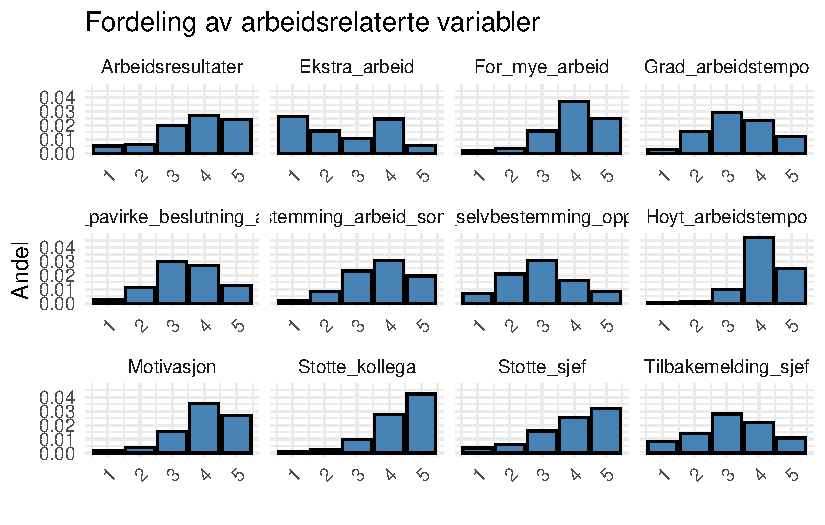
\includegraphics{kand_SOK2209_Bacheloroppgave_V25_files/figure-pdf/unnamed-chunk-19-1.pdf}

\begin{verbatim}
lavaan 0.6-19 ended normally after 90 iterations

  Estimator                                       DWLS
  Optimization method                           NLMINB
  Number of model parameters                        60

  Number of observations                          6103
  Number of missing patterns                         1

Model Test User Model:
                                              Standard      Scaled
  Test Statistic                              1679.341    1470.660
  Degrees of freedom                                80          80
  P-value (Chi-square)                           0.000       0.000
  Scaling correction factor                                  1.156
  Shift parameter                                           17.644
    simple second-order correction                                

Model Test Baseline Model:

  Test statistic                             27795.716   20453.789
  Degrees of freedom                                36          36
  P-value                                        0.000       0.000
  Scaling correction factor                                  1.360

User Model versus Baseline Model:

  Comparative Fit Index (CFI)                    0.942       0.932
  Tucker-Lewis Index (TLI)                       0.974       0.969
                                                                  
  Robust Comparative Fit Index (CFI)                            NA
  Robust Tucker-Lewis Index (TLI)                               NA

Root Mean Square Error of Approximation:

  RMSEA                                          0.057       0.053
  90 Percent confidence interval - lower         0.055       0.051
  90 Percent confidence interval - upper         0.060       0.056
  P-value H_0: RMSEA <= 0.050                    0.000       0.010
  P-value H_0: RMSEA >= 0.080                    0.000       0.000
                                                                  
  Robust RMSEA                                                  NA
  90 Percent confidence interval - lower                        NA
  90 Percent confidence interval - upper                        NA
  P-value H_0: Robust RMSEA <= 0.050                            NA
  P-value H_0: Robust RMSEA >= 0.080                            NA

Standardized Root Mean Square Residual:

  SRMR                                           0.035       0.035

Parameter Estimates:

  Parameterization                               Theta
  Standard errors                           Robust.sem
  Information                                 Expected
  Information saturated (h1) model        Unstructured

Latent Variables:
                   Estimate  Std.Err  z-value  P(>|z|)   Std.lv  Std.all
  Latent_JK =~                                                          
    For_mye_arbeid    1.000                               0.684    0.565
    Hoyt_arbedstmp    0.397    0.025   15.628    0.000    0.272    0.393
    Ekstra_arbeid     1.359    0.123   11.005    0.000    0.929    0.681
  Latent_JR =~                                                          
    Grd_slvbstmmn_    1.000                               1.023    0.715
    Grd_slvbst____    1.283    0.041   31.384    0.000    1.312    0.795
    Grad_arbedstmp    0.932    0.027   34.628    0.000    0.953    0.690
    Grd_pvrk_bslt_    1.060    0.031   34.023    0.000    1.084    0.735

Regressions:
                   Estimate  Std.Err  z-value  P(>|z|)   Std.lv  Std.all
  Motivasjon ~                                                          
    Latent_JR (a1)    0.479    0.019   25.304    0.000    0.490    0.430
    Form_qnrm (a2)    0.008    0.017    0.479    0.632    0.008    0.007
    ald_ung   (c1)   -0.363    0.045   -8.098    0.000   -0.363   -0.121
    ald_elder (c2)    0.253    0.041    6.192    0.000    0.253    0.093
    Kvinne    (c3)    0.013    0.033    0.406    0.685    0.013    0.006
    Utd_grnns (c4)    0.016    0.047    0.346    0.730    0.016    0.005
    Utd_nvrst (c5)   -0.016    0.035   -0.462    0.644   -0.016   -0.007
    Barn      (c6)    0.017    0.046    0.379    0.704    0.017    0.005
    arb_stlln (c7)    0.004    0.001    6.134    0.000    0.004    0.087
  logsyk ~                                                              
    Latent_JK (b1)    0.042    0.020    2.071    0.038    0.029    0.035
    Latent_JR (b2)   -0.087    0.013   -6.887    0.000   -0.089   -0.108
    Form_qnrm (b3)   -0.104    0.012   -9.015    0.000   -0.104   -0.123
    Motivasjn (b4)   -0.033    0.011   -2.951    0.003   -0.033   -0.046
    ald_ung   (g1)    0.010    0.029    0.344    0.731    0.010    0.005
    ald_elder (g2)    0.005    0.026    0.191    0.848    0.005    0.003
    Kvinne    (g3)    0.216    0.022    9.674    0.000    0.216    0.130
    Utd_grnns (g4)    0.037    0.030    1.230    0.219    0.037    0.015
    Utd_nvrst (g5)   -0.113    0.024   -4.709    0.000   -0.113   -0.066
    Barn      (g6)    0.042    0.030    1.411    0.158    0.042    0.018
    arb_stlln (g7)    0.002    0.000    3.356    0.001    0.002    0.045

Covariances:
                   Estimate  Std.Err  z-value  P(>|z|)   Std.lv  Std.all
  Latent_JK ~~                                                          
    Latent_JR        -0.071    0.013   -5.269    0.000   -0.101   -0.101

Intercepts:
                   Estimate  Std.Err  z-value  P(>|z|)   Std.lv  Std.all
   .Hoyt_arbedstmp    4.055    0.046   87.671    0.000    4.055    5.865
   .logsyk           -4.305    0.056  -77.022    0.000   -4.305   -5.213

Thresholds:
                   Estimate  Std.Err  z-value  P(>|z|)   Std.lv  Std.all
    For_mye_rbd|t1   -2.130    0.092  -23.078    0.000   -2.130   -1.758
    For_mye_rbd|t2   -1.481    0.086  -17.294    0.000   -1.481   -1.223
    For_mye_rbd|t3   -0.366    0.082   -4.458    0.000   -0.366   -0.302
    For_mye_rbd|t4    1.109    0.083   13.304    0.000    1.109    0.915
    Ekstra_arbd|t1   -0.100    0.094   -1.064    0.288   -0.100   -0.073
    Ekstra_arbd|t2    0.609    0.096    6.333    0.000    0.609    0.446
    Ekstra_arbd|t3    1.074    0.099   10.807    0.000    1.074    0.787
    Ekstra_arbd|t4    2.684    0.120   22.398    0.000    2.684    1.966
    Grd_slvbstm_|1   -1.820    0.100  -18.273    0.000   -1.820   -1.272
    Grd_slvbstm_|2   -0.406    0.097   -4.173    0.000   -0.406   -0.284
    Grd_slvbstm_|3    1.020    0.098   10.429    0.000    1.020    0.713
    Grd_slvbstm_|4    2.171    0.100   21.705    0.000    2.171    1.518
    Grd_slvb____|1   -2.894    0.127  -22.861    0.000   -2.894   -1.755
    Grd_slvb____|2   -1.469    0.118  -12.490    0.000   -1.469   -0.891
    Grd_slvb____|3    0.120    0.116    1.041    0.298    0.120    0.073
    Grd_slvb____|4    1.829    0.118   15.533    0.000    1.829    1.109
    Grd_rbdstmp|t1   -2.388    0.102  -23.526    0.000   -2.388   -1.729
    Grd_rbdstmp|t2   -0.884    0.096   -9.233    0.000   -0.884   -0.640
    Grd_rbdstmp|t3    0.497    0.095    5.204    0.000    0.497    0.360
    Grd_rbdstmp|t4    1.750    0.097   18.121    0.000    1.750    1.267
    Grd_pvrk_bs_|1   -2.398    0.105  -22.871    0.000   -2.398   -1.626
    Grd_pvrk_bs_|2   -0.896    0.096   -9.315    0.000   -0.896   -0.608
    Grd_pvrk_bs_|3    0.691    0.096    7.174    0.000    0.691    0.469
    Grd_pvrk_bs_|4    2.207    0.098   22.497    0.000    2.207    1.496
    Motivasjon|t1    -2.074    0.088  -23.694    0.000   -2.074   -1.820
    Motivasjon|t2    -1.417    0.079  -17.971    0.000   -1.417   -1.244
    Motivasjon|t3    -0.441    0.077   -5.724    0.000   -0.441   -0.387
    Motivasjon|t4     0.886    0.077   11.495    0.000    0.886    0.778

Variances:
                   Estimate  Std.Err  z-value  P(>|z|)   Std.lv  Std.all
   .For_mye_arbeid    1.000                               1.000    0.681
   .Hoyt_arbedstmp    0.404    0.007   57.258    0.000    0.404    0.845
   .Ekstra_arbeid     1.000                               1.000    0.537
   .Grd_slvbstmmn_    1.000                               1.000    0.489
   .Grd_slvbst____    1.000                               1.000    0.368
   .Grad_arbedstmp    1.000                               1.000    0.524
   .Grd_pvrk_bslt_    1.000                               1.000    0.460
   .Motivasjon        1.000                               1.000    0.770
   .logsyk            0.642    0.015   42.372    0.000    0.642    0.941
    Latent_JK         0.468    0.043   10.881    0.000    1.000    1.000
    Latent_JR         1.046    0.046   22.600    0.000    1.000    1.000

Scales y*:
                   Estimate  Std.Err  z-value  P(>|z|)   Std.lv  Std.all
    For_mye_arbeid    0.825                               0.825    1.000
    Ekstra_arbeid     0.733                               0.733    1.000
    Grd_slvbstmmn_    0.699                               0.699    1.000
    Grd_slvbst____    0.606                               0.606    1.000
    Grad_arbedstmp    0.724                               0.724    1.000
    Grd_pvrk_bslt_    0.678                               0.678    1.000
    Motivasjon        0.898                               0.898    1.000
\end{verbatim}

\begin{verbatim}
lavaan 0.6-19 ended normally after 93 iterations

  Estimator                                       DWLS
  Optimization method                           NLMINB
  Number of model parameters                        60

  Number of observations                          6103
  Number of missing patterns                         2

Model Test User Model:
                                              Standard      Scaled
  Test Statistic                              1656.220    1450.355
  Degrees of freedom                                80          80
  P-value (Chi-square)                           0.000       0.000
  Scaling correction factor                                  1.156
  Shift parameter                                           17.587
    simple second-order correction                                

Model Test Baseline Model:

  Test statistic                             27526.979   20379.516
  Degrees of freedom                                36          36
  P-value                                        0.000       0.000
  Scaling correction factor                                  1.351

User Model versus Baseline Model:

  Comparative Fit Index (CFI)                    0.943       0.933
  Tucker-Lewis Index (TLI)                       0.974       0.970
                                                                  
  Robust Comparative Fit Index (CFI)                            NA
  Robust Tucker-Lewis Index (TLI)                               NA

Root Mean Square Error of Approximation:

  RMSEA                                          0.057       0.053
  90 Percent confidence interval - lower         0.054       0.051
  90 Percent confidence interval - upper         0.059       0.055
  P-value H_0: RMSEA <= 0.050                    0.000       0.019
  P-value H_0: RMSEA >= 0.080                    0.000       0.000
                                                                  
  Robust RMSEA                                                  NA
  90 Percent confidence interval - lower                        NA
  90 Percent confidence interval - upper                        NA
  P-value H_0: Robust RMSEA <= 0.050                            NA
  P-value H_0: Robust RMSEA >= 0.080                            NA

Standardized Root Mean Square Residual:

  SRMR                                           0.035       0.035

Parameter Estimates:

  Parameterization                               Theta
  Standard errors                           Robust.sem
  Information                                 Expected
  Information saturated (h1) model        Unstructured

Latent Variables:
                   Estimate  Std.Err  z-value  P(>|z|)   Std.lv  Std.all
  Latent_JK =~                                                          
    For_mye_arbeid    1.000                               0.682    0.563
    Hoyt_arbedstmp    0.396    0.025   15.710    0.000    0.270    0.390
    Ekstra_arbeid     1.384    0.127   10.927    0.000    0.944    0.686
  Latent_JR =~                                                          
    Grd_slvbstmmn_    1.000                               1.021    0.715
    Grd_slvbst____    1.288    0.041   31.361    0.000    1.316    0.796
    Grad_arbedstmp    0.933    0.027   34.654    0.000    0.953    0.690
    Grd_pvrk_bslt_    1.060    0.031   34.008    0.000    1.083    0.735

Regressions:
                   Estimate  Std.Err  z-value  P(>|z|)   Std.lv  Std.all
  Motivasjon ~                                                          
    Latent_JR (a1)    0.480    0.019   25.303    0.000    0.490    0.430
    Form_qnrm (a2)    0.008    0.017    0.479    0.632    0.008    0.007
    ald_ung   (c1)   -0.363    0.045   -8.098    0.000   -0.363   -0.121
    ald_elder (c2)    0.253    0.041    6.192    0.000    0.253    0.093
    Kvinne    (c3)    0.013    0.033    0.406    0.685    0.013    0.006
    Utd_grnns (c4)    0.016    0.047    0.346    0.730    0.016    0.005
    Utd_nvrst (c5)   -0.016    0.035   -0.462    0.644   -0.016   -0.007
    Barn      (c6)    0.017    0.046    0.379    0.704    0.017    0.005
    arb_stlln (c7)    0.004    0.001    6.134    0.000    0.004    0.087
  logsyk_u0 ~                                                           
    Latent_JK (b1)    0.035    0.030    1.168    0.243    0.024    0.034
    Latent_JR (b2)   -0.025    0.018   -1.364    0.173   -0.025   -0.037
    Form_qnrm (b3)   -0.076    0.018   -4.330    0.000   -0.076   -0.108
    Motivasjn (b4)   -0.040    0.016   -2.444    0.015   -0.040   -0.066
    ald_ung   (g1)   -0.074    0.042   -1.772    0.076   -0.074   -0.041
    ald_elder (g2)    0.127    0.040    3.145    0.002    0.127    0.077
    Kvinne    (g3)    0.051    0.032    1.577    0.115    0.051    0.037
    Utd_grnns (g4)   -0.002    0.044   -0.048    0.962   -0.002   -0.001
    Utd_nvrst (g5)   -0.038    0.035   -1.085    0.278   -0.038   -0.027
    Barn      (g6)    0.033    0.042    0.787    0.431    0.033    0.017
    arb_stlln (g7)   -0.002    0.001   -2.188    0.029   -0.002   -0.049

Covariances:
                   Estimate  Std.Err  z-value  P(>|z|)   Std.lv  Std.all
  Latent_JK ~~                                                          
    Latent_JR        -0.070    0.013   -5.243    0.000   -0.100   -0.100

Intercepts:
                   Estimate  Std.Err  z-value  P(>|z|)   Std.lv  Std.all
   .Hoyt_arbedstmp    4.055    0.046   87.671    0.000    4.055    5.865
   .logsyk_u0        -2.960    0.072  -41.002    0.000   -2.960   -4.299

Thresholds:
                   Estimate  Std.Err  z-value  P(>|z|)   Std.lv  Std.all
    For_mye_rbd|t1   -2.128    0.092  -23.090    0.000   -2.128   -1.758
    For_mye_rbd|t2   -1.480    0.086  -17.298    0.000   -1.480   -1.223
    For_mye_rbd|t3   -0.365    0.082   -4.458    0.000   -0.365   -0.302
    For_mye_rbd|t4    1.108    0.083   13.311    0.000    1.108    0.915
    Ekstra_arbd|t1   -0.101    0.095   -1.064    0.288   -0.101   -0.073
    Ekstra_arbd|t2    0.613    0.097    6.326    0.000    0.613    0.446
    Ekstra_arbd|t3    1.082    0.100   10.777    0.000    1.082    0.787
    Ekstra_arbd|t4    2.703    0.122   22.155    0.000    2.703    1.966
    Grd_slvbstm_|1   -1.818    0.100  -18.273    0.000   -1.818   -1.272
    Grd_slvbstm_|2   -0.406    0.097   -4.173    0.000   -0.406   -0.284
    Grd_slvbstm_|3    1.019    0.098   10.429    0.000    1.019    0.713
    Grd_slvbstm_|4    2.169    0.100   21.705    0.000    2.169    1.518
    Grd_slvb____|1   -2.900    0.127  -22.859    0.000   -2.900   -1.755
    Grd_slvb____|2   -1.472    0.118  -12.489    0.000   -1.472   -0.891
    Grd_slvb____|3    0.121    0.116    1.041    0.298    0.121    0.073
    Grd_slvb____|4    1.832    0.118   15.532    0.000    1.832    1.109
    Grd_rbdstmp|t1   -2.388    0.101  -23.532    0.000   -2.388   -1.729
    Grd_rbdstmp|t2   -0.884    0.096   -9.234    0.000   -0.884   -0.640
    Grd_rbdstmp|t3    0.497    0.095    5.204    0.000    0.497    0.360
    Grd_rbdstmp|t4    1.750    0.097   18.118    0.000    1.750    1.267
    Grd_pvrk_bs_|1   -2.396    0.105  -22.867    0.000   -2.396   -1.626
    Grd_pvrk_bs_|2   -0.896    0.096   -9.315    0.000   -0.896   -0.608
    Grd_pvrk_bs_|3    0.691    0.096    7.174    0.000    0.691    0.469
    Grd_pvrk_bs_|4    2.205    0.098   22.503    0.000    2.205    1.496
    Motivasjon|t1    -2.074    0.088  -23.694    0.000   -2.074   -1.820
    Motivasjon|t2    -1.417    0.079  -17.971    0.000   -1.417   -1.244
    Motivasjon|t3    -0.441    0.077   -5.724    0.000   -0.441   -0.387
    Motivasjon|t4     0.886    0.077   11.495    0.000    0.886    0.778

Variances:
                   Estimate  Std.Err  z-value  P(>|z|)   Std.lv  Std.all
   .For_mye_arbeid    1.000                               1.000    0.683
   .Hoyt_arbedstmp    0.405    0.007   57.520    0.000    0.405    0.848
   .Ekstra_arbeid     1.000                               1.000    0.529
   .Grd_slvbstmmn_    1.000                               1.000    0.489
   .Grd_slvbst____    1.000                               1.000    0.366
   .Grad_arbedstmp    1.000                               1.000    0.524
   .Grd_pvrk_bslt_    1.000                               1.000    0.460
   .Motivasjon        1.000                               1.000    0.770
   .logsyk_u0         0.459    0.016   28.127    0.000    0.459    0.968
    Latent_JK         0.465    0.043   10.915    0.000    1.000    1.000
    Latent_JR         1.043    0.046   22.589    0.000    1.000    1.000

Scales y*:
                   Estimate  Std.Err  z-value  P(>|z|)   Std.lv  Std.all
    For_mye_arbeid    0.826                               0.826    1.000
    Ekstra_arbeid     0.727                               0.727    1.000
    Grd_slvbstmmn_    0.700                               0.700    1.000
    Grd_slvbst____    0.605                               0.605    1.000
    Grad_arbedstmp    0.724                               0.724    1.000
    Grd_pvrk_bslt_    0.679                               0.679    1.000
    Motivasjon        0.898                               0.898    1.000
\end{verbatim}

\newpage

\section{Analyse}\label{analyse}

Vi bruker den definerte modellen i \ref{sec-metode} ved hjelp at pakken
Lavaan i R, og i vurdering av resultatene våre tar vi utgangspunkt i
\ref{teori}.

forklare estimator = ``WLSMV'', parameterization = ``theta'',

forklare hva tallene i tabellen betyr etter transformasjonene

\subsubsection{Tabell med resultat fra
regresjonsanalysen(e)}\label{tabell-med-resultat-fra-regresjonsanalysene}

\begin{table}[htbp]
\centering
\caption{Resultater fra strukturmodellen (Modell 1) for prediksjon av motivasjon og sykefravær (\texttt{logsyk}).}
\label{tab:sem_results_model1}
\begin{tabular}{@{}llrrrrc@{}}
\toprule
Avhengig variabel & Prediktor & Estimat & Std.Err & z-verdi & p-verdi & Std.all \\
\midrule
\multicolumn{7}{l}{\textit{Prediktorer for motivasjon}} \\
& \texttt{Latent\_JR} (a1) & 0.479 & 0.019 & 25.304 & <0.001 & 0.430 \\
& \texttt{Formue\_qnorm} (a2) & 0.008 & 0.017 & 0.479 & 0.632 & 0.007 \\
& \texttt{ald\_ung} (c1) & -0.363 & 0.045 & -8.098 & <0.001 & -0.121 \\
& \texttt{ald\_elder} (c2) & 0.253 & 0.041 & 6.192 & <0.001 & 0.093 \\
& \texttt{Kvinne} (c3) & 0.013 & 0.033 & 0.406 & 0.685 & 0.006 \\
& \texttt{Utd\_grunnskole} (c4) & 0.016 & 0.047 & 0.346 & 0.730 & 0.005 \\
& \texttt{Utd\_universitet} (c5) & -0.016 & 0.035 & -0.462 & 0.644 & -0.007 \\
& \texttt{Barn} (c6) & 0.017 & 0.046 & 0.379 & 0.704 & 0.005 \\
& \texttt{arb\_stillingspst} (c7) & 0.004 & 0.001 & 6.134 & <0.001 & 0.087 \\
\midrule
\multicolumn{7}{l}{\textit{Prediktorer for sykefravær (\texttt{logsyk})}} \\
& \texttt{Latent\_JK} (b1) & 0.042 & 0.020 & 2.071 & 0.038 & 0.035 \\
& \texttt{Latent\_JR} (b2) & -0.087 & 0.013 & -6.887 & <0.001 & -0.108 \\
& \texttt{Formue\_qnorm} (b3) & -0.104 & 0.012 & -9.015 & <0.001 & -0.123 \\
& \texttt{Motivasjon} (b4) & -0.033 & 0.011 & -2.951 & 0.003 & -0.046 \\
& \texttt{ald\_ung} (g1) & 0.010 & 0.029 & 0.344 & 0.731 & 0.005 \\
& \texttt{ald\_elder} (g2) & 0.005 & 0.026 & 0.191 & 0.848 & 0.003 \\
& \texttt{Kvinne} (g3) & 0.216 & 0.022 & 9.674 & <0.001 & 0.130 \\
& \texttt{Utd\_grunnskole} (g4) & 0.037 & 0.030 & 1.230 & 0.219 & 0.015 \\
& \texttt{Utd\_universitet} (g5) & -0.113 & 0.024 & -4.709 & <0.001 & -0.066 \\
& \texttt{Barn} (g6) & 0.042 & 0.030 & 1.411 & 0.158 & 0.018 \\
& \texttt{arb\_stillingspst} (g7) & 0.002 & 0.000 & 3.356 & 0.001 & 0.045 \\
\bottomrule
\end{tabular}
\footnotesize{\textit{Merk:} Estimat er ustandardisert koeffisient. Std.Err er standardfeil. Std.all er fullstendig standardisert koeffisient. Referansekategorier: Alder (30–54 år), Utdanning (videregående). \texttt{Formue\_qnorm} er normalisert formue. \texttt{arb\_stillingspst} er sentrert stillingsprosent. \texttt{logsyk} er log(sykefravær + 0.01).}
\end{table}

\subsubsection{Resultat knyttet til
hypoteser}\label{resultat-knyttet-til-hypoteser}

\subsection{Prediksjon av log-transformert
sykefravær}\label{prediksjon-av-log-transformert-sykefravuxe6r}

\subsubsection{Hypotese 1}\label{hypotese-1}

Vi finner en positiv og statistisk signifikant sammenheng mellom
\textbf{Jobbkrav (\texttt{Latent\_JK})} og \texttt{logsyk} (Estimat =
\(0.042\), Std.all = \(0.035\), \(p = 0.038\)). Dette gir støtte til H1.
Økte jobbkrav er assosiert med en økning i log-transformert sykefravær.
Effekten er relativt liten, men signifikant.

\subsubsection{Hypotese 2}\label{hypotese-2}

Det er en negativ og statistisk signifikant sammenheng mellom
Jobbressurser (Latent\_JR) og logsyk (Estimat = \(-0.087\), Std.all =
\(-0.108\), \(p < 0.001\)). Dette gir i utgangspunktet sterk støtte til
H2. Økt tilgang på jobbressurser er assosiert med en reduksjon i
log-transformert sykefravær.

\subsubsection{Hypotese 3}\label{hypotese-3}

Formue (Formue\_qnorm) viser en negativ og statistisk signifikant
sammenheng med logsyk (Estimat = \(-0.104\), Std.all = \(-0.123\),
\(p < 0.001\)). Dette gir sterk støtte til H3. Et høyere formuenivå
(målt på en normalisert skala) er assosiert med en reduksjon i
log-transformert sykefravær, selv når vi kontrollerer for jobbkrav,
jobbressurser og motivasjon.

\subsection{Prediksjon av motivasjon}\label{prediksjon-av-motivasjon}

\subsubsection{Hypotese 4}\label{hypotese-4}

Som vist i øvre del av \autoref{tab:sem_results_model1}, er
Jobbressurser (Latent\_JR) en sterk og positiv prediktor for Motivasjon
(Estimat = \(0.479\), Std.all = \(0.430\), \(p < 0.001\)). Dette er i
tråd med JD-R-modellen, som postulerer at ressurser i jobben fremmer en
motiverende prosess. Formue (Formue\_qnorm) viser derimot ingen
signifikant direkte sammenheng med Motivasjon (Estimat = \(0.008\),
\(p = 0.632\)). Vår antakelse om at formue direkte påvirker motivasjon
får dermed ikke støtte i denne modellen og H3

\subsubsection{Redegjørelse for effekt av
kontrollvariabler}\label{redegjuxf8relse-for-effekt-av-kontrollvariabler}

\subsubsection{Redegjørelse for svakheter i
modellen/data}\label{redegjuxf8relse-for-svakheter-i-modellendata}

Til å starte med så er denne typen modell i grensepunktet på vår
forståelse og dette fører til at det må tilføyes usikkerhet til
tolkningen av resultatene. Spesielt gjelder dette for forståelsen av
modelltilpasning, estimatorjusteringer og tolkning av latente
sammenhenger i strukturelle ligningsmodeller med kategoriske data. Selv
om analysen bygger på anerkjent metode og teori, er SEM med latente
variabler og robuste estimatorer som WLSMV et metodisk nivå som ligger i
ytterkanten av hva vi på bachelor nivå kan tolke. Resultatene diskuteres
derfor med forsiktighet, og vi legger vekt på overordnede mønstre
fremfor detaljerte tolkninger.

Siden sykefraværet er så høyreskjevt selv når det er log-transformert,
kan det gi oss p-verdier som er for lave, og dermed kan det være at vi
overestimerer effekten av prediktorene.

Hvis vi ekskluderer de uten legemeldt sykefravær og log-transformerer
sykefraværet uten å legge til 0.01, slik at det er tilnærmet
normalfordelt, så kan vi se om dette endrer resultatene. Dette er gjort
i modell 2, og vi ser at det er store endringer i resultatene.

\begin{table}[htbp]
\centering
\caption{Resultater fra strukturmodellen (Modell 2) for prediksjon av motivasjon og sykefravær (\texttt{logsyk\_u0}).}
\label{tab:sem_results_model2}
\begin{tabular}{@{}llrrrrc@{}}
\toprule
Avhengig variabel & Prediktor & Estimat & Std.Err & z-verdi & p-verdi & Std.all \\
\midrule
\multicolumn{7}{l}{\textit{Prediktorer for motivasjon}} \\
& \texttt{Latent\_JR} (a1) & 0.480 & 0.019 & 25.303 & <0.001 & 0.430 \\
& \texttt{Formue\_qnorm} (a2) & 0.008 & 0.017 & 0.479 & 0.632 & 0.007 \\
& \texttt{ald\_ung} (c1) & -0.363 & 0.045 & -8.098 & <0.001 & -0.121 \\
& \texttt{ald\_elder} (c2) & 0.253 & 0.041 & 6.192 & <0.001 & 0.093 \\
& \texttt{Kvinne} (c3) & 0.013 & 0.033 & 0.406 & 0.685 & 0.006 \\
& \texttt{Utd\_grunnskole} (c4) & 0.016 & 0.047 & 0.346 & 0.730 & 0.005 \\
& \texttt{Utd\_universitet} (c5) & -0.016 & 0.035 & -0.462 & 0.644 & -0.007 \\
& \texttt{Barn} (c6) & 0.017 & 0.046 & 0.379 & 0.704 & 0.005 \\
& \texttt{arb\_stillingspst} (c7) & 0.004 & 0.001 & 6.134 & <0.001 & 0.087 \\
\midrule
\multicolumn{7}{l}{\textit{Prediktorer for sykefravær (\texttt{logsyk\_u0})}} \\
& \texttt{Latent\_JK} (b1) & 0.035 & 0.030 & 1.168 & 0.243 & 0.034 \\
& \texttt{Latent\_JR} (b2) & -0.025 & 0.018 & -1.364 & 0.173 & -0.037 \\
& \texttt{Formue\_qnorm} (b3) & -0.076 & 0.018 & -4.330 & <0.001 & -0.108 \\
& \texttt{Motivasjon} (b4) & -0.040 & 0.016 & -2.444 & 0.015 & -0.066 \\
& \texttt{ald\_ung} (g1) & -0.074 & 0.042 & -1.772 & 0.076 & -0.041 \\
& \texttt{ald\_elder} (g2) & 0.127 & 0.040 & 3.145 & 0.002 & 0.077 \\
& \texttt{Kvinne} (g3) & 0.051 & 0.032 & 1.577 & 0.115 & 0.037 \\
& \texttt{Utd\_grunnskole} (g4) & -0.002 & 0.044 & -0.048 & 0.962 & -0.001 \\
& \texttt{Utd\_universitet} (g5) & -0.038 & 0.035 & -1.085 & 0.278 & -0.027 \\
& \texttt{Barn} (g6) & 0.033 & 0.042 & 0.787 & 0.431 & 0.017 \\
& \texttt{arb\_stillingspst} (g7) & -0.002 & 0.001 & -2.188 & 0.029 & -0.049 \\
\bottomrule
\end{tabular}
\footnotesize{\textit{Merk:} Estimat er ustandardisert koeffisient. Std.Err er standardfeil. Std.all er fullstendig standardisert koeffisient. Referansekategorier: Alder (30–54 år), Utdanning (videregående). \texttt{Formue\_qnorm} er normalisert formue. \texttt{arb\_stillingspst} er sentrert stillingsprosent. \texttt{logsyk\_u0} er log(sykefravær) for respondenter med sykefravær > 0.}
\end{table}

\newpage

\section{Resultat}\label{resultat}

Her presenteres den empiriske analysen og dens resultater. Vanligvis vil
en empirisk analyse bestå av en regresjonsanalyse med flere variabler.
Andre muligheter kan diskuteres med veilederen.

\subsection{Tabeller}\label{tabeller}

\subsection{Figurer}\label{figurer}

\subsection{Forklaring av tabeller og
figurer}\label{forklaring-av-tabeller-og-figurer}

\newpage

\section{Diskusjon}\label{diskusjon}

\paragraph{får se om vi beholder
dette}\label{fuxe5r-se-om-vi-beholder-dette}

Karrierevalg og utdanning fra gallup som viste en fattigere har
dårligere tilgang på ``career role models'' som gjør at de kanskje ikke
vet om de bedre yrkene og sånt og dermed igjen blir mindre utdanna og
sånt https://www.gallup.com/analytics/506696/amazon-research-hub.aspx så
effekt på karriærevalg, utdanning osv. langsiktig effekt av
formue/bakrunn er noe påvirker hvilken type jobb folk har og dermed
jobbkrav og jobbresssurser. Dette er da en indirekte effekt som vi ikke
får med.

\subsubsection{Formueeffekt på konsum}\label{formueeffekt-puxe5-konsum}

https://fnce.wharton.upenn.edu/wp-content/uploads/2019/08/chodorowreich-crns\_stock\_wealth\_effects.pdf

for hver dollar i formue du har så har du 0.028usd mer i konsum eller
noe

https://usa.visa.com/partner-with-us/visa-consulting-analytics/economic-insights/the-sudden-increase-in-the-wealth-effect-and-its-impact-on-spending.html

så vi kan vise til hvordan de med lav formue da kan være tvungen til å
ta mer tima selv med lav motivasjon for samme konsumnivå fant det
tilfeldigvis her
https://www.economist.com/finance-and-economics/2025/03/19/the-trump-administration-is-playing-a-dangerous-stockmarket-game

\subsubsection{Motivasjonseffekt av
ulikhet}\label{motivasjonseffekt-av-ulikhet}

``The motivational cost of inequality: Opportunity gaps reduce the
willingness to work'' https://pmc.ncbi.nlm.nih.gov/articles/PMC7473543/

https://www.brookings.edu/articles/income-inequality-social-mobility-and-the-decision-to-drop-out-of-high-school/

ulikhet gjør at fattige blir mindre motivert siden dem føler det å bli
rik er ``umulig'' og dermed investerer mindre i seg -\textgreater{}
lavere motivasjon og lavere utdanning. kanskje mer fysisk arbeid.

så formue har effekt på hvor mye utdanning du har. formue har effekt på
hvilken motivasjon du har. formue har effekt på m som er annen inntekt
utenom jobb.

Dette kapitlet drøfter resultatene i forhold til problemstillingen. Hva
er funnet ut av, hva gjenstår, hvilke styrker og svakheter har analysen?

\subsubsection{Oppsummering av hva formålet med oppgaven var, og hva
analysen
viste}\label{oppsummering-av-hva-formuxe5let-med-oppgaven-var-og-hva-analysen-viste}

\subsubsection{Diskusjon av hvilke konklusjoner som kan trekkes fra
dette og om resultatene er forenlig med tidligere
funn/teori}\label{diskusjon-av-hvilke-konklusjoner-som-kan-trekkes-fra-dette-og-om-resultatene-er-forenlig-med-tidligere-funnteori}

\subsubsection{Diskusjon av svakheter i
analysen}\label{diskusjon-av-svakheter-i-analysen}

\subsubsection{Diskusjon av implikasjoner for policy gitt
svakheter}\label{diskusjon-av-implikasjoner-for-policy-gitt-svakheter}

\subsubsection{Eventuelt: diskusjon av hva framtidig forskning kan
forske videre på (basert påderes funn og svakheter i
analysen)}\label{eventuelt-diskusjon-av-hva-framtidig-forskning-kan-forske-videre-puxe5-basert-puxe5deres-funn-og-svakheter-i-analysen}

Formues påvirkning på avtalte timer og ikke-lineære effekter. Vi har en
antakelse om at formue potensielt kan ha en effekt på avtalte timer, som
igjen vil påvirke sykefraværet. Dette fremstår som en mer intrikat
sammenheng enn det vi har hatt rom for å utforske, utover å inkludere
stillingsprosent som en kontrollvariabel. Dette representerer en svakhet
ved den nåværende modellen. Fremtidige studier kunne med fordel
undersøke denne mekanismen nærmere.

I teori i \autoref{sec-formue-jdr} så vi at effekten av formue på
sykefravær kan være ikke lineær eller evt bue formet. Vår nåværende
modell har primært antatt lineære sammenhenger for formues direkte
roller (utenom den normaliserte transformasjonen av formuevariabelen i
seg selv).

Basert på dette, og inspirert av tidligere ideer som ikke ble fullt ut
testet i denne omgang, ser vi flere konkrete områder for videre
utforskning:

Interaksjon mellom stillingsprosent og formue: Vi har ikke testet
hvordan formue eventuelt endrer effekten av arbeidstimer (representert
ved stillingsprosent, på sykefravær. JD-R-modellen understreker at
jobbkrav kan tære på helsen. Det er imidlertid uklart om en økonomisk
buffer i form av høyere formue kan dempe den negative effekten av høy
arbeidsbelastning. Individer med lav formue har ofte mindre
fleksibilitet til å justere arbeidstempo eller jobbe redusert ved
slitasje. De med høyere formue kan derimot i større grad ha mulighet til
å velge jobber med høyt timeantall som også tilbyr bedre
restitusjonsmuligheter eller andre kompenserende faktorer.

Videre forskning: En fremtidig studie burde vurdere et eksplisitt
interaksjonsledd mellom (sentrert) stillingsprosent og formue. Målet
ville være å undersøke om den potensielt positive sammenhengen mellom
stillingsprosent og sykefravær, kanskje blir svakere (eller til og med
snur) ved økende formuesnivå.

Formues indirekte påvirkning på sykefravær via motivasjon: Vi har antatt
at formue kan påvirke sykefravær indirekte gjennom arbeidsmotivasjon.
Forventningen er at høyere formue kan bidra til økt motivasjon ved å
redusere finansiell usikkerhet og skape positive fremtidsutsikter (en
positiv effekt, a2\textgreater0 i vår motivasjonsmodell,
\autoref{eq:motivasjon}). Videre, i tråd med funn som hos Langseth-Eide
\& Vittersø (2021), kan høyere motivasjon og engasjement tenkes å
redusere sykefraværet (en negativ effekt i vår sykefraværsmodell.

Videre forskning: Selv om vår nåværende SEM-modell estimerer disse
separate stiene, og en indirekte effekt kan beregnes, behandlet vi
motivasjon som en enkel observert variabel basert på ett spørsmål.
Fremtidig arbeid kunne med fordel teste en mer utdypende
medieringsmodell hvor motivasjon kanskje operasjonaliseres som en latent
variabel basert på flere indikatorer. Det vil være sentralt å kartlegge
mer robust om økt formue faktisk styrker ulike fasetter av motivasjon
(f.eks. indre vs.~ytre), og om denne motivasjonsøkningen i sin tur har
en signifikant og substansiell fraværsreduserende effekt.

Ikke-lineær moderering av jobbkrav med formue: JD-R-modellen forutsetter
ofte en lineær effekt av jobbkrav på utfall som stress eller sykefravær.
Vi har i våre tidligere betraktninger tenkt at formue kunne moderere
denne sammenhengen lineært.

Videre forskning: I virkeligheten kan det tenkes at individer med svært
lav formue er spesielt sensitive for økte jobbkrav, grunnet frykt for
tap av inntektsmulighet og forverret helse. Samtidig kan formues
buffereffekt flate ut på svært høye formuesnivåer (de rikeste opplever
kanskje uansett lite fravær relatert til jobbstress, uavhengig av små
variasjoner i jobbkrav). Det kan også være at de med aller lavest formue
mister motivasjon dersom opplevd ulikhet og manglende muligheter blir
for store. Fremtidige studier bør derfor utforske potensielle
ikke-lineære modereringseffekter. Dette kan innebære å teste
interaksjonsledd som tillater effekten av jobbkrav å variere på en mer
kompleks måte med formuesnivået, for eksempel ved å bruke
spline-funksjoner for formue i interaksjonen, eller ved å sammenligne
effekter på tvers av flere, mer detaljerte formueskategorier.

Avtagende grensenytte av jobbressurser for de med høy formue:
JJobbressurser antas å fungere beskyttende, men effekten kan tenkes å
avta med økende formue. De med lav formue kan få relativt større utbytte
av ekstra støtte, autonomi og påvirkningsmulighet fordi de har mindre
økonomisk spillerom og færre alternative buffere. De med høy formue har
allerede en betydelig buffer, så den marginale gevinsten av ytterligere
jobbressurser kan være mindre.

Videre forskning: Dette kan testes mer inngående, ikke bare med et
lineært interaksjonsledd mellom jobbressurser og formue (hvor man ville
forvente en positiv koeffisient hvis den negative effekten av
jobbressurser på sykefravær svekkes med økende formue), men også ved å
undersøke effekter separat for ulike formuessegmenter (f.eks. laveste,
midterste og høyeste kvintil/kvartil av formuesfordelingen) for å se om
styrken på sammenhengen mellom jobbressurser og sykefravær varierer
systematisk.

Ulike operasjonaliseringer og dimensjoner av formue: Vi har benyttet
bruttofinanskapital, transformert til en normalfordeling (Z-skåre). Det
er imidlertid sannsynlig at ulike typer formue kan ha ulik psykologisk
betydning og dermed ulik effekt. For eksempel kan nettoformue (som tar
hensyn til gjeld), sammensetningen av formuen (boligformue
vs.~verdipapirformue), eller kilden til formuen (arvet vs.~opparbeidet)
spille forskjellig inn på opplevd trygghet og handlingsrom. En person
med betydelig boligformue, men også høy gjeld, opplever kanskje mindre
reell økonomisk trygghet enn en med tilsvarende bruttoformue plassert i
likvide midler.

Videre forskning: Fremtidige studier bør derfor utforske og sammenligne
ulike formuemål for å se om typen formue modererer effekten av jobbkrav
og jobbressurser på ulike måter.

\begin{verbatim}
Differensiering av jobbkrav og -ressurser:
Vi har operert med relativt brede latente skalaer for jobbkrav (inkludert arbeidsmengde, tidspress, ekstra arbeid) og jobbressurser (inkludert støtte, autonomi, påvirkning). Teoretisk sett er det mulig at formue modererer effekten av ulike spesifikke dimensjoner av krav og ressurser forskjellig.

    Videre forskning: Kan formue i større grad dempe effekten av fysiske belastninger enn emosjonelle krav? Eller kan høy formue paradoksalt nok føre til høyere personlige ambisjoner og krav til egen prestasjon, som delvis nøytraliserer fordelene av økte ressurser? Fremtidige studier kunne med fordel dekomponere disse brede konstruktene for å undersøke slike nyanserte interaksjoner.
\end{verbatim}

\newpage

\section*{Referanser}\label{referanser}

\phantomsection\label{refs}
\begin{CSLReferences}{1}{0}
\bibitem[\citeproctext]{ref-demerouti2001job}
Demerouti, E., Bakker, A. B., Nachreiner, F. \& Schaufeli, W. B. (2001).
The job demands-resources model of burnout. \emph{Journal of Applied
Psychology}, \emph{86}(3), 499.

\bibitem[\citeproctext]{ref-durlauf_2022_the}
Durlauf, S. N., Kourtellos, A. \& Tan, C. M. (2022). The great gatsby
curve. \emph{Annual Review of Economics}, \emph{14}.
\url{https://doi.org/10.1146/annurev-economics-082321-122703}

\bibitem[\citeproctext]{ref-cfpbconsumerfinancialprotectionbureau_2015_financial}
Financial Protection Bureau), C. (Consumer. (2015). \emph{Financial
well-being: The goal of financial education}.
https://www.consumerfinance.gov/.
\url{https://files.consumerfinance.gov/f/201501_cfpb_report_financial-well-being.pdf}

\bibitem[\citeproctext]{ref-gesiarz2020motivational}
Gesiarz, F., De Neve, J.-E. \& Sharot, T. (2020). The motivational cost
of inequality: Opportunity gaps reduce the willingness to work.
\emph{Plos One}, \emph{15}(9), e0237914.

\bibitem[\citeproctext]{ref-gugushvili2025wealth}
Gugushvili, A. \& Wiborg, Ø. N. (2025). Wealth and mortality among
late-middle-aged individuals in norway: A nationwide register-based
retrospective study. \emph{The Lancet Regional Health--Europe},
\emph{48}.

\bibitem[\citeproctext]{ref-hattrem_hvor}
Hattrem, A. (n.d.). \emph{Hvor mange er fattige i norge?} SSB. Retrieved
May 23, 2025, from
\url{https://www.ssb.no/inntekt-og-forbruk/inntekt-og-formue/artikler/hvor-mange-er-fattige-i-norge}

\bibitem[\citeproctext]{ref-hobfoll1989conservation}
Hobfoll, S. E. (1989). Conservation of resources: A new attempt at
conceptualizing stress. \emph{American Psychologist}, \emph{44}(3), 513.

\bibitem[\citeproctext]{ref-jaeggi2021wealth}
Jaeggi, A. V., Blackwell, A. D., Von Rueden, C., Trumble, B. C.,
Stieglitz, J., Garcia, A. R., Kraft, T. S., Beheim, B. A., Hooper, P.
L., Kaplan, H., et al. (2021). Do wealth and inequality associate with
health in a small-scale subsistence society? \emph{Elife}, \emph{10},
e59437.

\bibitem[\citeproctext]{ref-langseth2019s}
Langseth-Eide, B. (2019). It's been a hard day's night and i've been
working like a dog: Workaholism and work engagement in the JD-r model.
\emph{Frontiers in Psychology}, \emph{10}, 1444.

\bibitem[\citeproctext]{ref-langseth2021ticket}
Langseth-Eide, B. \& Vittersø, J. (2021). Ticket to ride: A longitudinal
journey to health and work-attendance in the jd-r model.
\emph{International Journal of Environmental Research and Public
Health}, \emph{18}(8), 4327.

\bibitem[\citeproctext]{ref-normann_2009_inntektsfattig}
Normann, T. M. (2009). \emph{Inntektsfattig eller levekårsfattig?}
ssb.no.
\url{https://www.ssb.no/sosiale-forhold-og-kriminalitet/artikler-og-publikasjoner/inntektsfattig-eller-levekaarsfattig}

\bibitem[\citeproctext]{ref-pickett2015income}
Pickett, K. E. \& Wilkinson, R. G. (2015). Income inequality and health:
A causal review. \emph{Social Science \& Medicine}, \emph{128},
316--326.

\bibitem[\citeproctext]{ref-JSSv048i02}
Rosseel, Y. (2012). Lavaan: An r package for structural equation
modeling. \emph{Journal of Statistical Software}, \emph{48}(2), 1--36.
\url{https://doi.org/10.18637/jss.v048.i02}

\bibitem[\citeproctext]{ref-schaufeli2004job}
Schaufeli, W. B. \& Bakker, A. B. (2004). Job demands, job resources,
and their relationship with burnout and engagement: A multi-sample
study. \emph{Journal of Organizational Behavior: The International
Journal of Industrial, Occupational and Organizational Psychology and
Behavior}, \emph{25}(3), 293--315.

\bibitem[\citeproctext]{ref-ssb2024beregnet}
SSB. (2017). \emph{Beregnet bruttofinanskapital}.
\url{https://www.ssb.no/a/metadata/conceptvariable/vardok/3449/nb}

\bibitem[\citeproctext]{ref-unguren2021moderator}
Üngüren, E., Tekin, Ö. A., Avsallı, H. \& Kaçmaz, Y. Y. (2021). The
moderator role of financial well-being on the effect of job insecurity
and the COVID-19 anxiety on burnout: A research on hotel-sector
employees in crisis. \emph{Sustainability}, \emph{13}, 9031.
\url{https://doi.org/10.3390/su13169031}

\bibitem[\citeproctext]{ref-vander2016job}
Vander Elst, T., Cavents, C., Daneels, K., Johannik, K., Baillien, E.,
Van den Broeck, A. \& Godderis, L. (2016). Job demands--resources
predicting burnout and work engagement among belgian home health care
nurses: A cross-sectional study. \emph{Nursing Outlook}, \emph{64}(6),
542--556.

\bibitem[\citeproctext]{ref-zucman2019global}
Zucman, G. (2019). Global wealth inequality. \emph{Annual Review of
Economics}, \emph{11}(1), 109--138.

\end{CSLReferences}

\newpage

\section*{Vedlegg}\label{vedlegg}

Her legger vi til vår QMD fil.

\section*{Appendiks}\label{appendiks}

\subsection*{Kode}\label{kode}

\subsection*{Tester}\label{tester}

\subsection*{Kunstig intelligens}\label{kunstig-intelligens}



\end{document}
